\documentclass[%
 %reprint,
  twocolumn,
 %superscriptaddress,
 %groupedaddress,
 %unsortedaddress,
 %runinaddress,
 %frontmatterverbose,
 % preprint,
 showpacs,
 showkeys,
 preprintnumbers,
 %nofootinbib,
 %nobibnotes,
 %bibnotes,
 amsmath,amssymb,
 aps,
 % prl,
 pra,
 % prb,
 % rmp,
 %prstab,
 %prstper,
  longbibliography,
 %floatfix,
 %lengthcheck,%
 ]{revtex4-1}

%\usepackage{cdmtcs-pdf}

\usepackage[dvipsnames]{xcolor}

\usepackage{mathptmx}% http://ctan.org/pkg/mathptmx

\usepackage{amssymb,amsthm,amsmath,bm}

\usepackage{tikz}
\usetikzlibrary{calc,decorations.pathreplacing,decorations.markings,positioning,shapes}

\usepackage[breaklinks=true,colorlinks=true,anchorcolor=blue,citecolor=blue,filecolor=blue,menucolor=blue,pagecolor=blue,urlcolor=blue,linkcolor=blue]{hyperref}
\usepackage{graphicx}% Include figure files
\usepackage{url}

\usepackage{mathbbol} %%%% for \mathds{1}

\begin{document}

\title{Generalized Greenberger-Horne-Zeilinger arguments from quantum logical analysis}


\author{Karl Svozil}
\email{svozil@tuwien.ac.at}
\homepage{http://tph.tuwien.ac.at/~svozil}

\affiliation{Institute for Theoretical Physics,
Vienna  University of Technology,
Wiedner Hauptstrasse 8-10/136,
1040 Vienna,  Austria}


\date{\today}

\begin{abstract}
The Greenberger-Horne-Zeilinger (GHZ) argument against noncontextual local hidden variables is recast in quantum logical terms of fundamental propositions, states and probabilities. Unlike Kochen-Specker- and Hardy-like configurations, this operator based argument proceeds within four nonintertwining contexts. The nonclassical performance of the GHZ argument is due to the choice or filtering of observables with respect to a particular state. We study the varieties of GHZ games one could play in these four contexts, depending on the chosen state of the GHZ basis.
\end{abstract}

\keywords{Greenberger-Horne-Zeilinger argument, Gleason theorem, Kochen-Specker theorem, Born rule, gadget graphs, Greechie diagram, McKay-Megill-Pavicic diagram (MMP), orthogonality hypergraph}
\pacs{03.65.Ca, 02.50.-r, 02.10.-v, 03.65.Aa, 03.67.Ac, 03.65.Ud}

\maketitle


% MDPI  \PassOptionsToPackage{dvipsnames}{xcolor}
% MDPI  \documentclass[entropy,article,submit,oneauthor,pdftex]{Definitions/mdpi}
% MDPI
% MDPI
% MDPI  %%%%%%%%%%%%%%%%%%%%%%%%%%%%%%%%%%%%%%%%%%%%%%%%%%%%%%%%%%%%%%%%%%%%%%%%%%%%%%%%%%%%%%%%%%%%%%%%%%%%%%%%%%%%%%%%%%%%%%%%%%%%%%%%%%%%%%%%%%%%%%%%
% MDPI  \usepackage{graphicx}% Include figure files
% MDPI
% MDPI  \usepackage{amssymb}
% MDPI
% MDPI  \usepackage{tikz}
% MDPI  \usetikzlibrary{calc,decorations.pathreplacing,decorations.markings,positioning,shapes}
% MDPI
% MDPI  \newcommand{\ruledtabular}{\hline \hline}
% MDPI
% MDPI  %%%%%%%%%%%%%%%%%%%%%%%%%%%%%%%%%%%%%%%%%%%%%%%%%%%%%%%%%%%%%%%%%%%%%%%%%%%%%%%%%%%%%%%%%%%%%%%%%%%%%%%%%%%%%%%%%%%%%%%%%%%%%%%%%%%%%%%%%%%%%%%%
% MDPI
% MDPI
% MDPI
% MDPI  \firstpage{1}
% MDPI  \makeatletter
% MDPI  \setcounter{page}{\@firstpage}
% MDPI  \makeatother
% MDPI  \pubvolume{xx}
% MDPI  \issuenum{1}
% MDPI  \articlenumber{5}
% MDPI  \pubyear{2019}
% MDPI  \copyrightyear{2019}
% MDPI  %\externaleditor{Academic Editor: name}
% MDPI  %\history{Received: date; Accepted: date; Published: date}
% MDPI  %\updates{yes} % If there is an update available, un-comment this line
% MDPI
% MDPI  %% MDPI internal command: uncomment if new journal that already uses continuous page numbers
% MDPI  %\continuouspages{yes}
% MDPI
% MDPI  %------------------------------------------------------------------
% MDPI  % The following line should be uncommented if the LaTeX file is uploaded to arXiv.org
% MDPI  %\pdfoutput=1
% MDPI
% MDPI  %=================================================================
% MDPI  % Add packages and commands here. The following packages are loaded in our class file: fontenc, calc, indentfirst, fancyhdr, graphicx, lastpage, ifthen, lineno, float, amsmath, setspace, enumitem, mathpazo, booktabs, titlesec, etoolbox, amsthm, hyphenat, natbib, hyperref, footmisc, geometry, caption, url, mdframed, tabto, soul, multirow, microtype, tikz
% MDPI
% MDPI  %=================================================================
% MDPI  %% Please use the following mathematics environments: Theorem, Lemma, Corollary, Proposition, Characterization, Property, Problem, Example, ExamplesandDefinitions, Hypothesis, Remark, Definition, Notation, Assumption
% MDPI  %% For proofs, please use the proof environment (the amsthm package is loaded by the MDPI class).
% MDPI
% MDPI  %=================================================================
% MDPI  % Full title of the paper (Capitalized)
% MDPI  \Title{Classical predictions for intertwined quantum observables are contingent and thus inconclusive}
% MDPI  %\thanks{This is a largely revised and extended version of a paper which has been published somewhat hidden in Section~12.9 of my recent book on (A)Causality~\cite{svozil-pac}.}
% MDPI
% MDPI  % Author Orchid ID: enter ID or remove command
% MDPI  \newcommand{\orcidauthorA}{0000-0001-6554-2802} % Add \orcidA{} behind the author's name
% MDPI
% MDPI  % Authors, for the paper (add full first names)
% MDPI  \Author{Karl Svozil $^{1}$*}
% MDPI
% MDPI  % Authors, for metadata in PDF
% MDPI  \AuthorNames{Karl Svozil}
% MDPI
% MDPI  % Affiliations / Addresses (Add [1] after \address if there is only one affiliation.)
% MDPI  \address{$^{1}$ \quad Institute for Theoretical Physics, Vienna University of Technology, Wiedner Hauptstrasse 8-10/136, A-1040 Vienna, Austria, EU; svozil@tuwien.ac.at}
% MDPI
% MDPI  % Contact information of the corresponding author
% MDPI  %\corres{Correspondence: e-mail@e-mail.com; Tel.: (optional; include country code; if there are multiple corresponding authors, add author initials) +xx-xxxx-xxx-xxxx (F.L.)}
% MDPI
% MDPI  % Current address and/or shared authorship
% MDPI  %\firstnote{Current address: Affiliation 3}
% MDPI  %\secondnote{These authors contributed equally to this work.}
% MDPI  % The commands \thirdnote{} till \eighthnote{} are available for further notes
% MDPI
% MDPI  %\simplesumm{} % Simple summary
% MDPI
% MDPI  %\conference{} % An extended version of a conference paper
% MDPI
% MDPI  % Abstract (Do not insert blank lines, i.e. \\)
% MDPI  \abstract{Classical evaluations of configurations of intertwined quantum contexts induce relations, such as true-implies-false, true-implies-true~\cite{2018-minimalYIYS}, but also nonseparability among the input and output terminals. When combined, these exploitable configurations (aka gadgets) deliver the strongest form of classical value indefiniteness. However, the choice of the respective configuration among all such collections, and thus the relation of its terminals, remains arbitrary and cannot be motivated by some superselection principle inherent to quantum or classical physics.}
% MDPI  % Keywords
% MDPI  \keyword{Quantum mechanics, Gleason theorem, Kochen-Specker theorem, Born rule, gadget graphs}
% MDPI
% MDPI  % The fields PACS, MSC, and JEL may be left empty or commented out if not applicable
% MDPI  \PACS{03.65.Ca, 02.50.-r, 02.10.-v, 03.65.Aa, 03.67.Ac, 03.65.Ud}
% MDPI  %\MSC{}
% MDPI  %\JEL{}
% MDPI
% MDPI  %%%%%%%%%%%%%%%%%%%%%%%%%%%%%%%%%%%%%%%%%%
% MDPI  % Only for the journal Diversity
% MDPI  %\LSID{\url{http://}}
% MDPI
% MDPI  %%%%%%%%%%%%%%%%%%%%%%%%%%%%%%%%%%%%%%%%%%
% MDPI  % Only for the journal Applied Sciences:
% MDPI  %\featuredapplication{Authors are encouraged to provide a concise description of the specific application or a potential application of the work. This section is not mandatory.}
% MDPI  %%%%%%%%%%%%%%%%%%%%%%%%%%%%%%%%%%%%%%%%%%
% MDPI
% MDPI  %%%%%%%%%%%%%%%%%%%%%%%%%%%%%%%%%%%%%%%%%%
% MDPI  % Only for the journal Data:
% MDPI  %\dataset{DOI number or link to the deposited data set in cases where the data set is published or set to be published separately. If the data set is submitted and will be published as a supplement to this paper in the journal Data, this field will be filled by the editors of the journal. In this case, please make sure to submit the data set as a supplement when entering your manuscript into our manuscript editorial system.}
% MDPI
% MDPI  %\datasetlicense{license under which the data set is made available (CC0, CC-BY, CC-BY-SA, CC-BY-NC, etc.)}
% MDPI
% MDPI  %%%%%%%%%%%%%%%%%%%%%%%%%%%%%%%%%%%%%%%%%%
% MDPI  % Only for the journal Toxins
% MDPI  %\keycontribution{The breakthroughs or highlights of the manuscript. Authors can write one or two sentences to describe the most important part of the paper.}
% MDPI
% MDPI  %\setcounter{secnumdepth}{4}
% MDPI  %%%%%%%%%%%%%%%%%%%%%%%%%%%%%%%%%%%%%%%%%%
% MDPI \begin{document}

\setcounter{MaxMatrixCols}{20}

\section{Quantum logical structures}

In what follows, the Greenberger-Horne-Zeilinger (GHZ) argument~\cite{ghz}
will be recast in purely quantum logical terms.
In particular, the operators corresponding to GHZ observables will be written in their spectral form,
such that the respective orthogonal projection operators can be identified with elementary propositions.
Since the argument is state-dependent, the appropriate states need to be identified,
and their predictions and expectations on those elementary propositions need to be evaluated.
This facilitates the discernment of important structural components.
Such insights can then be used to embed and relate GHZ to traditional quantum logical findings,
as well as to generalize and extend the argument to more general experimentally verifiable predictions and assertions.

\subsection{Appraisal}

The configuration of observables and states that constitute a
GHZ argument
renders a capacity to perform on specific tasks (although it is worse for other tasks, see Section~\ref{2020-ghz-gtcbwbcbnbqm})
that no classical means can achieve:
It lets three parties ``win'' a particular task with certainty,
whereas there is only a probabilistic classical chance to do so classically.

The situation is not unlike the quantum Deutsch algorithm~\cite[Section~2.2]{mermin-07}:
It yields a particular property (parity) of the input with one query with certainty,
whereas there is only a probabilistic classical chance to do so classically.

There are potential drawbacks though since this performance increase is not ``universal''.
Because on the one hand, other tasks can only be achieved by invoking different states and operators;
and, on the other hand, ``complete'' determination of some unknown
quantum state (without preselection) requires the same number of queries as in the classical case.
As a result, the capacity of such algorithms is problem and query-specific.
Yet, as long as one is interested in increasing capabilities or performance
not universally but for a particular task or ``game''
such quantum advantages exist and are exploitable.

What ``drives'' GHZ is quantum entanglement: the capacity to relationally encode~\cite{schrodinger-gwsidqm2,zeil-99} multi- (in this case three-) partite systems
in such a way that the (information of the) properties of the constituents are defined merely as their collective behavior.
Again, there is a price involved, in this case, the complete loss of (information of the) properties of the individual constituents.
Indeed, for pure states individual and relational properties can be rewritten into each other by nonlocal ``scrambling''
unitary transformations ``sampling'' individual into relational states~\cite{svozil-2016-sampling}.
Such entangled states can ``carry''  relational information about collective properties of their constituents
that no classical state can.

\subsection{Motivation for logico-algebraic analysis}

As mentioned earlier the GHZ argument will be very explicitly analyzed in terms of its quantum logical aspects;
in particular, concerning the observables and states involved.
One advantage of such an analysis is accessibility to other fields of research,
as it appears less ad hoc and complementing existing research.

It might not be too unreasonable to state that, for classical-versus-quantum discord, the GHZ argument ``competes'' with
the  Kochen-Specker (KS) theorem~\cite{kochen1},
even though the latter can be converted into the former~\cite{Xu-Chen-Guehnw-2020,cabello2020converting}.
Whereas the KS theorem, as well as its weaker probabilistic form,
the Hardy-type argument~\cite{Hardy-93,svozil-2020-hardy} (sometimes referred to as 1-implies-$\{0,1\}$~\cite{svozil-2006-omni} or true-implies-\{false.true\}-rule~\cite{2018-minimalYIYS})
often is ``local'', GHZ uses a particular three-partite configuration whose constituents can be space-like separated.

KS and Hardy-type configurations use elementary dichotomic yes-no or 0--1 propositions
(which can be encoded as a normalized vector $\vert {\bf a} \rangle$ (in three or higher dimensions)
spanning a one-dimensional subspace of the Hilbert space,
and which is equivalent to the orthogonal projection operator $\vert {\bf a} \rangle \langle {\bf a}\vert $
projecting the Hilbert space onto this subspace).
In contradistinction, GHZ use expectations of three dichotomic variables, each of which assumes either the value 1 or -1,
and triple distributions.

Thereby, the GHZ argument is operator-based~\cite{Holweck2017},
because it allows observables and their associated self-adjoint operators with eigenvalues
``$+1$'' and ``$-1$''---that should be understood in terms of their spectral forms as functions of orthogonal projection operators
occurring in the KS and Hardy-type configurations.
(Functions of normal operators can be defined  by their spectral form~\cite[\S~82, p.~165-169]{halmos-vs}.)
In what follows we shall also find that, whereas the KS argument involves many intricately intertwining contexts,
the~GHZ argument uses a single isolated context.

\section{Classical GHZ games}

Routine approaches to classical-versus-quantum discord start from some collection of quantum observables
and attempt to force classical interpretations upon them.
In contrast to this manners the GHZ argument will be motivated by
the lack of capacity to perform certain tasks by classical means,
whereas quantum capacities to achieve these tasks exist.
The presentation starts with an exposition by
Bacon (aka ``The Quantum Pontiff'')~\cite{bacon-ghzgames-2006} (see also Refs.~\cite{Broadbent-PRNLboxes,Scarani-prboxes})
in which certain quantum resources allow players always to win,
whereas this cannot be guaranteed classically.


Suppose some prison ward allows three parties to pre-select some ``share'', and subsequently isolates them in separate cells
(without further communication).
Afterward, the ward distributes paper slips to each one of them, such that each slip contains a single symbol out of two symbols -- say, ``$x$'' or ``$y$'' -- per party and slip,
in either one of the following four configurations or contexts: $xxx$, $xyy$, $yxy$, and $yyx$ (the order reflects the order of the parties).
In particular, the ward does not reveal which type of configuration is chosen,
so from the intrinsic ``local'' perception of the single isolated prisoners,
upon reception of ``$x$'' or ``$y$'' it could be two different configurations or contexts
(the possibility of the other two configurations can be eliminated by exclusion).
Upon receiving the slip, all three parties must then write on their slips (or shout) simultaneously and without any further coordination either ``$-$''1 or ``$+$''1.

\subsection{Positive products from squares of outcomes}
Suppose the goal is, in algebraic terms, to form negative products of these three factors for all four configurations $xxx$, $xyy$, $yxy$, and $yyx$.
Does there exist a ``classical strategy'' for those players to always win? Yes, because by a parity argument, if one forms
$
\underbrace{(x \cdot x\cdot x)}_{-1}
\cdot
\underbrace{(x\cdot y\cdot y)}_{-1}
\cdot
\underbrace{(y\cdot x\cdot y)}_{-1}
\cdot
\underbrace{(y\cdot y\cdot x)}_{-1} = (-1)^4=1$---and
thereby multiplies all factors of all of the four configurations---one
obtains $x^6 y^6$ which allows a classical strategy of writing (or shouting)
``$-$''1 on $x$, and anything (but previously coordinated and fixed), that is, ``$\pm$''1 on $y$.
More explicitly, suppose the prisoners have agreed to write (or shout) ``$-1$'' for $x$ and ``$+1$'' for $y$;
then
$
\underbrace{(\overbrace{x}^{-1} \cdot \overbrace{x}^{-1}\cdot \overbrace{x}^{-1})}_{-1}
=
\underbrace{(\overbrace{x}^{-1}\cdot \overbrace{y}^{+1}\cdot \overbrace{y}^{+1})}_{-1}
=
\underbrace{(\overbrace{y}^{+1}\cdot \overbrace{x}^{-1}\cdot \overbrace{y}^{+1})}_{-1}
=
\underbrace{(\overbrace{y}^{+1}\cdot \overbrace{y}^{+1}\cdot \overbrace{x}^{-1})}_{-1}$
and the prisoners always win.
Very similar considerations apply to requests of the prison ward to produce only positive results,
or more general demands that will be discussed later.

\subsection{GHZ goal: negative products from squares of outcomes}
However, some goals for the prisoners are unachievable by classical means.
In particular, let us specify the GHZ game as the goal set by the prison ward as follows:
``produce the products
$x \cdot x\cdot x = +1$ and  $x\cdot y\cdot y=y\cdot x\cdot y=y\cdot y\cdot x=-1$.''
Then, by the same parity argument mentioned earlier, the prisoners cannot win all the time, since then the combined product
$
\underbrace{(x \cdot x\cdot x)}_{+1}
\cdot
\underbrace{(x\cdot y\cdot y)}_{-1}
\cdot
\underbrace{(y\cdot x\cdot y)}_{-1}
\cdot
\underbrace{(y\cdot y\cdot x)}_{-1}
=(+1)(-1)^3=-1$
would be negative but the respective factors occur in multiples of squares $x^2$ and $y^2$ and
must therefore result in a positive product---a perfect contradiction.
Note that the earlier strategy of writing (or shouting) ``$-$''1 on $x$, and anything, that is, ``$\pm$''1 on $y$
would still succeed whenever the ward invokes slips that carry $xyy$, $yxy$, and $yyx$ on them.
But this strategy fails miserably in the positive $xxx$ case.
Conversely, the ``inverse'' strategy  of writing (or shouting) ``$+$''1 on $x$, and anything, that is, ``$\pm$''1 on $y$
would succeed in the positive $xxx$ case
but fail for all other cases requesting negative products $xyy$, $yxy$, and $yyx$.

Note that if the ward would also reveal the configuration chosen then all of these games could easily be won by the prisoners
with classical means,
albeit not in a context-invariant or context-independent way.
Because then, from each of the four classical configurations or contexts, they could choose a single instance that would fit
the game---say, $x_+x_+x_+$ for the $xxx$ configuration, and $x_-y_+y_+$, $y_+x_-y_+$, and $y_+y_+x_-$ for the other three configurations---and thereby
win the earlier game not recoverable by classical noncontextual means.
Here the context dependence is in the $x$ assignments: ``$+$''1 for the $xxx$ configuration, ``$-$''1
for the other configurations $xyy$, $yxy$, and $yyx$.

However, this nondisclosure of configurations and contexts is not how the GHZ game has been operationalized and empirically presented~\cite{PhysRevLett.82.1345,panbdwz}.
There, the final configuration or context $xxx$ [which supposedly serves as a criterion for (non)classicality]
is not subjected to a ``delayed-choice'' involving space-like separated events.
Therefore, this performance could in principle also be rendered classically by noncontextual value assignments discussed later.


Nevertheless, the original GHZ protocol offers a quantum method for the prisoners to win all the time---that is, for all cases
the ward may choose---without disclosing the chosen configuration or context to the prisoners.
But before going into this particular realization, the classical case will be formalized a little further.

\subsection{Contexts involved in classical GHZ configurations}


We shall argue that the classical Shimony-Mermin form~\cite{ghsz,mermin90b,mermin} of the GHZ argument employs four separate nonintertwining ``complementary'' contexts.
For the sake of the argument suppose one is dealing with classical objects, such as generalized urn models~\cite{wright} or finite automata~\cite{svozil-2001-eua,svozil-2018-b}
which encode (a classical form of) complementarity.
Alternatively one might think of just classical objects which can have two dichotomic properties, namely
the dichotomic observables
\begin{equation}
{{x}} \in \{x_+,x_-\}     \textrm{, and }  {{y}} \in \{y_+,y_-\}
,
\label{2020-ghz-hl}
\end{equation}
where $x_+$ and $x_-$ as well as $y_+$ and $y_-$ are the states corresponding to outcomes of measurements of ${{x}}$ and ${{y}}$, respectively.

Suppose further that one is drawing triples of identical balls from a generalized urn.
Consider four types of measurements on the first, second and third ball:
\begin{equation}
 \{  {{x}} , {{x}} , {{x}}  \}
,
 \{  {{x}} , {{y}} , {{y}}  \}
,
 \{  {{y}} , {{x}} , {{y}}  \}
, \textrm{ and }
 \{  {{y}} , {{y}} , {{x}}  \}
.
\label{2020-ghz-ghlm}
\end{equation}


In what follows, we shall use (conformal, orthogonality) hypergraphs~\cite[Sect.~2.4]{Bretto-MR3077516} introduced by Greechie~\cite[p.~120]{greechie:71}
that depict
logical configurations or
contexts as smooth lines~\cite{Greechie1968,kalmbach-83,svozil-tkadlec,Mckay2000,Pavicic-2005,Bretto-MR3077516,2018-minimalYIYS}.
The term hypergraph should be understood in the broadest possible consistent sense.
Figure~\ref{2020-f-ghz-contextconf}(a) represents the six Boolean algebras
associated with the propositional structures of six single-particle observables:
there are three particles, each measured at two angles or directions, respectively.
Simultaneous ``triple'' measurements of one (of two, either $x$ or $y$) observable per particle, on the three particles,
result in $2^3=8$ Cartesian product triples
forming the configurations or contexts
$\{x,x,x\}$,
$\{x,x,y\}$,
$\ldots$,
$\{y,y,y\}$.
Only four of these configurations or contexts, namely
$\{x,x,x\}$,
$\{x,y,y\}$,
$\{y,x,y\}$, and
$\{y,y,x\}$,
are employed in the GHZ argument.
Figure~\ref{2020-f-ghz-contextconf}(b) represents the eight possibilities, cases or instantiations per type of measurement
of the latter four GHZ contexts
(enumerated in lexicographic order; for brevity
we shall write ``${{a}}{{b}}{{c}}$''
for the ordered triple ``$\left[ {{a}},{{b}},{{c}} \right]$'').
\begin{equation}
\begin{aligned}
C_\textrm{c,GHZ}^{{{x}}{{x}}{{x}}}=& \{ x_+x_+x_+,x_+x_+x_-,x_+x_-x_+,x_+x_-x_-,\\ &\qquad x_-x_+x_+,x_-x_+x_-,x_-x_-x_+,x_-x_-x_- \}
,    \\
C_\textrm{c,GHZ}^{{{x}}{{y}}{{y}}}=& \{ x_+y_+y_+,x_+y_+y_-,x_+y_-y_+,x_+y_-y_-,\\ &\qquad x_-y_+y_+,x_-y_+y_-,x_-y_-y_+,x_-y_-y_- \}
,        \\
C_\textrm{c,GHZ}^{{{y}}{{x}}{{y}}}=& \{ y_+x_+y_+,y_+x_+y_-,y_+x_-y_+,y_+x_-y_-,\\ &\qquad y_-x_+y_+,y_-x_+y_-,y_-x_-y_+,y_-x_-y_- \}
, \textrm{ and}  \\
C_\textrm{c,GHZ}^{{{y}}{{y}}{{x}}}=& \{ y_+y_+x_+,y_+y_+x_-,y_+y_-x_+,y_+y_-x_-,\\ &\qquad y_-y_+x_+,y_-y_+x_-,y_-y_-x_+,y_-y_-x_- \}
.
\end{aligned}
\label{2020-ghz-ghlmcontexpl}
\end{equation}
which, bundeled into a set, are identified with the set of four~GHZ contexts
\begin{equation}
%\begin{aligned}
 \Big\{
C_\textrm{c,GHZ}^{{{x}}{{x}}{{x}}}
,
C_\textrm{c,GHZ}^{{{x}}{{y}}{{y}}}
,
C_\textrm{c,GHZ}^{{{y}}{{x}}{{y}}}
,
C_\textrm{c,GHZ}^{{{y}}{{y}}{{x}}}
\Big\}
.
%\end{aligned}
\label{2020-ghz-clghzc}
\end{equation}

\begin{figure}[htb]%[H]
\begin{center}
\begin{tabular}{ c }
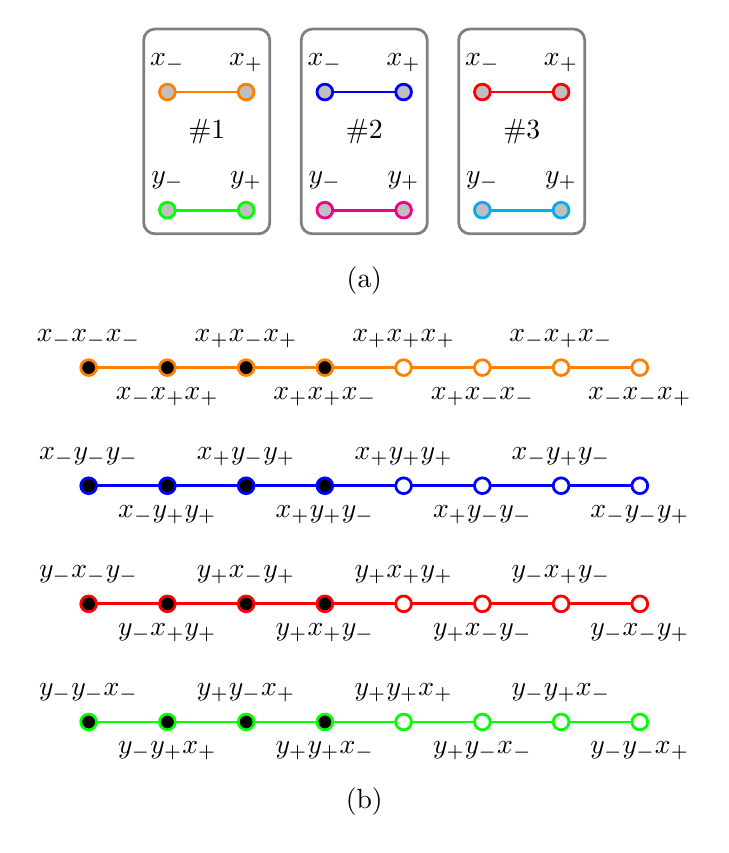
\begin{tikzpicture}  [scale=1]

\tikzstyle{every path}=[line width=1pt]

\newdimen\ms
\ms=0.1cm
\tikzstyle{s1}=[color=red,rectangle,inner sep=3.5]
\tikzstyle{c3}=[circle,inner sep={\ms/8},minimum size=4*\ms]
\tikzstyle{c2}=[circle,inner sep={\ms/8},minimum size=3*\ms]
\tikzstyle{c1}=[circle,inner sep={\ms/8},minimum size=2*\ms]
\tikzstyle{cs1}=[circle,inner sep={\ms/8},minimum size=1*\ms]

% Define positions of all observables


\coordinate (x11) at (1,8);
\coordinate (x12) at (2,8);
\coordinate (x21) at (3,8);
\coordinate (x22) at (4,8);
\coordinate (x31) at (5,8);
\coordinate (x32) at (6,8);

\coordinate (y11) at (1,6.5);
\coordinate (y12) at (2,6.5);
\coordinate (y21) at (3,6.5);
\coordinate (y22) at (4,6.5);
\coordinate (y31) at (5,6.5);
\coordinate (y32) at (6,6.5);

% draw contexts


\draw [color=orange] (x11) -- (x12);
\draw [color=blue] (x21) -- (x22);
\draw [color=red] (x31) -- (x32);
\draw [color=green] (y11) -- (y12);
\draw [color=magenta] (y21) -- (y22);
\draw [color=cyan] (y31) -- (y32);

% draw atoms

\draw (x11) coordinate[c1,fill=Gray!50, draw=orange,label=above:$x_-$];
\draw (x12) coordinate[c1,fill=Gray!50, draw=orange,label=above:$x_+$];
\draw (x21) coordinate[c1,fill=Gray!50, draw=blue,label=above:$x_-$];
\draw (x22) coordinate[c1,fill=Gray!50, draw=blue,label=above:$x_+$];
\draw (x31) coordinate[c1,fill=Gray!50, draw=red,label=above:$x_-$];
\draw (x32) coordinate[c1,fill=Gray!50, draw=red,label=above:$x_+$];

\draw (y11) coordinate[c1,fill=Gray!50, draw=green,label=above:$y_-$];
\draw (y12) coordinate[c1,fill=Gray!50, draw=green,label=above:$y_+$];
\draw (y21) coordinate[c1,fill=Gray!50, draw=magenta,label=above:$y_-$];
\draw (y22) coordinate[c1,fill=Gray!50, draw=magenta,label=above:$y_+$];
\draw (y31) coordinate[c1,fill=Gray!50, draw=cyan,label=above:$y_-$];
\draw (y32) coordinate[c1,fill=Gray!50, draw=cyan,label=above:$y_+$];

\draw[Gray,rounded corners] (0.70, 6.2) rectangle (2.30, 8.80) node[black,pos=.5] {{\#}1};
\draw[Gray,rounded corners] (2.70, 6.2) rectangle (4.30, 8.80) node[black,pos=.5] {{\#}2};
\draw[Gray,rounded corners] (4.70, 6.2) rectangle (6.30, 8.80) node[black,pos=.5] {{\#}3};

\coordinate (a) at (3.5,5.3);
\draw (a) coordinate[label=above:(a)];


% Define positions of all observables

\coordinate (ccu) at (0,4.5);
\coordinate (ccv) at (1,4.5);
\coordinate (cdu) at (2,4.5);
\coordinate (cdv) at (3,4.5);
\coordinate (dcu) at (4,4.5);
\coordinate (dcv) at (5,4.5);
\coordinate (ddu) at (6,4.5);
\coordinate (ddv) at (7,4.5);

\coordinate (cuc) at (0,3);
\coordinate (cvc) at (1,3);
\coordinate (cud) at (2,3);
\coordinate (cvd) at (3,3);
\coordinate (duc) at (4,3);
\coordinate (dvc) at (5,3);
\coordinate (dud) at (6,3);
\coordinate (dvd) at (7,3);

\coordinate (ucc) at (0,1.5);
\coordinate (vcc) at (1,1.5);
\coordinate (ucd) at (2,1.5);
\coordinate (vcd) at (3,1.5);
\coordinate (udc) at (4,1.5);
\coordinate (vdc) at (5,1.5);
\coordinate (udd) at (6,1.5);
\coordinate (vdd) at (7,1.5);

\coordinate (uuu) at (0,0);
\coordinate (uuv) at (1,0);
\coordinate (uvu) at (2,0);
\coordinate (uvv) at (3,0);
\coordinate (vuu) at (4,0);
\coordinate (vuv) at (5,0);
\coordinate (vvu) at (6,0);
\coordinate (vvv) at (7,0);

% draw contexts

\draw [color=orange] (ccu) -- (ddv);
\draw [color=blue] (cuc) -- (dvd);
\draw [color=red] (ucc) -- (vdd);
\draw [color=green] (uuu) -- (vvv);



% draw atoms

\draw (ccu) coordinate[c1,fill=black, draw=orange,label=above:$x_-  x_-  x_- $];
\draw (ccv) coordinate[c1,fill=black, draw=orange,label=below:$x_-  x_+  x_+ $];
\draw (cdu) coordinate[c1,fill=black, draw=orange,label=above:$x_+  x_-  x_+ $];
\draw (cdv) coordinate[c1,fill=black, draw=orange,label=below:$x_+  x_+  x_- $];
\draw (dcu) coordinate[c1,fill=white, draw=orange,label=above:$x_+  x_+  x_+     $];
\draw (dcv) coordinate[c1,fill=white, draw=orange,label=below:$x_+  x_-  x_-     $];
\draw (ddu) coordinate[c1,fill=white, draw=orange,label=above:$x_-  x_+  x_-     $];
\draw (ddv) coordinate[c1,fill=white, draw=orange,label=below:$x_-  x_-  x_+     $];

  \draw (cuc) coordinate[c1,fill=black, draw=blue,label=above:$x_-  y_-  y_- $];
  \draw (cvc) coordinate[c1,fill=black, draw=blue,label=below:$x_-  y_+  y_+ $];
  \draw (cud) coordinate[c1,fill=black, draw=blue,label=above:$x_+  y_-  y_+ $];
  \draw (cvd) coordinate[c1,fill=black, draw=blue,label=below:$x_+  y_+  y_- $];
  \draw (duc) coordinate[c1,fill=white, draw=blue,label=above:$x_+  y_+  y_+     $];
  \draw (dvc) coordinate[c1,fill=white, draw=blue,label=below:$x_+  y_-  y_-     $];
  \draw (dud) coordinate[c1,fill=white, draw=blue,label=above:$x_-  y_+  y_-     $];
  \draw (dvd) coordinate[c1,fill=white, draw=blue,label=below:$x_-  y_-  y_+     $];

   \draw (ucc) coordinate[c1,fill=black, draw=red,label=above:$y_-  x_-  y_- $];
   \draw (vcc) coordinate[c1,fill=black, draw=red,label=below:$y_-  x_+  y_+ $];
   \draw (ucd) coordinate[c1,fill=black, draw=red,label=above:$y_+  x_-  y_+ $];
   \draw (vcd) coordinate[c1,fill=black, draw=red,label=below:$y_+  x_+  y_- $];
   \draw (udc) coordinate[c1,fill=white, draw=red,label=above:$y_+  x_+  y_+     $];
   \draw (vdc) coordinate[c1,fill=white, draw=red,label=below:$y_+  x_-  y_-     $];
   \draw (udd) coordinate[c1,fill=white, draw=red,label=above:$y_-  x_+  y_-     $];
   \draw (vdd) coordinate[c1,fill=white, draw=red,label=below:$y_-  x_-  y_+     $];

 \draw (uuu) coordinate[c1,fill=black, draw=green,label=above:$y_-  y_-  x_- $];
 \draw (uuv) coordinate[c1,fill=black, draw=green,label=below:$y_-  y_+  x_+ $];
 \draw (uvu) coordinate[c1,fill=black, draw=green,label=above:$y_+  y_-  x_+ $];
 \draw (uvv) coordinate[c1,fill=black, draw=green,label=below:$y_+  y_+  x_- $];
 \draw (vuu) coordinate[c1,fill=white, draw=green,label=above:$y_+  y_+  x_+     $];
 \draw (vuv) coordinate[c1,fill=white, draw=green,label=below:$y_+  y_-  x_-     $];
 \draw (vvu) coordinate[c1,fill=white, draw=green,label=above:$y_-  y_+  x_-     $];
 \draw (vvv) coordinate[c1,fill=white, draw=green,label=below:$y_-  y_-  x_+     $];

\coordinate (b) at (3.5,-0.7);
\draw (b) coordinate[label=below:(b)];

\end{tikzpicture}
\end{tabular}
\end{center}
\caption{\label{2020-f-ghz-contextconf}
Hypergraphs representing
(a) the six disconnected classical single-particle contexts representing the observables of the first, second, and third particle, respectively;
(b) four isolated, nonintertwining contexts, with eight atoms each, employed in the GHZ argument
(there are eight contexts in total, but only half of them are considered).
Filled circles indicate states which are classically allowed in a modified GHZ game
requesting negativity for all products  $xyy=yxy=yyx=xxx=-1$.
Every column represents a viable noncontextual winning strategy.
}
\end{figure}


Suppose that $x_+$, $x_-$, $y_+$ and $y_-$ are real nonvanishing numbers.
The outcomes are multiplied, such that $[a,b,c]=a\times b\times c$.
Multiplication of the observables in the four contexts results in a bound from below:
\begin{equation}
({{x}}{{x}}{{x}})
({{x}}{{y}}{{y}})
({{y}}{{x}}{{y}})
({{y}}{{y}}{{x}})
 =
({{x}}{{y}})^6 >0.
\label{2020-ghz-ghlmcont}
\end{equation}
In particular, if one identifies $x_+=y_+=1$ and $x_-=y_-=-1$ then $[({{x}}{{y}})^3]^2 =1$.
As already pointed out earlier, this classical prediction rests upon a parity argument:
any square, indeed any even exponent, of a nonzero real number is positive.
Note also that, by taking the product of the first three terms,
one obtains $\left[(\pm x)^2(\pm y)^2\right]^3={{y}}^6  {{x}}^3 =  {{x}}^3 $.
This should always be identical to the last term  in~(\ref{2020-ghz-ghlmcont}),
which is ${{x}}{{x}}{{x}}$.
Because according to the classical assumption of noncontextuality---independence of the observed value of ${{x}}$
on whatever other observables are measured simultaneously alongside it in different configurations or contexts---and
value definiteness, it should not make any difference
in which of the four contexts in~(\ref{2020-ghz-ghlmcont})
${{x}}$ is measured.
This, and the equivalent bound from below
in~(\ref{2020-ghz-ghlmcont}), are the classical predictions.


The classical probabilities of this configuration are the convex summations of $4^3$ extreme cases
from the 4 individual cases
$\{x_+y_+,x_+y_-,x_-y_+,x_-y_-\}$
per one of the three particles.
If interpreted geometrically  these $4^3$ vertices in six-dimensional space,
and their equivalent representations in terms of inequalities of the hull of the
convex polytope spanned by them, has been enumerated for three-partite correlations~\cite{2000-poly}.
In all $4^3$ classical cases, and for all classical probability distributions constructed from them, prediction~(\ref{2020-ghz-ghlmcont}) is satisfied.

Note that the classical GHZ contexts are isolated from each other and do not ``communicate''
via common intertwine observables.
As has been pointed out earlier,
in this aspect, they differ from other KS or Hardy-type arguments involving gadgets of intertwining contexts.

\section{Quantum advantage}

Let us now turn to quantum mechanical predictions of quantum doubles of the classical configuration of contexts introduced earlier;
in particular to a GHZ configuration that yields a winning strategy to the classical GHZ game
goal set by the prison ward as follows:
``produce the products
$x \cdot x\cdot x = +1$ and  $x\cdot y\cdot y=y\cdot x\cdot y=y\cdot y\cdot x=-1$.''
This is a rewrite of a confifuration that was presented
by Greenberger, Horne and Zeilinger~\cite{ghz},
later with Shimony~\cite{ghsz}.
(I still vividly remember that earlier Zeilinger
had suggested to me to pursue  ``a three-particle analog of the Bell-type two-particle setup'' but I had cordially abstained.)
Immediately afterward Mermin gave a uniform presentation of the GHZ argument~\cite{mermin90b,mermin1}
that can readily be rewritten in terms of the underlying elementary propositions,
a task which is pursued here.
Subsequently, these quantum predictions have been empirically confirmed~\cite{PhysRevLett.82.1345,panbdwz};
albeit with some provisos which will be discussed later.

By a quantum realization is some identification of (i) the observables ${{x}}$ and ${{y}}$
with self-adjoint operators; in particular, with two-times-two Hermitian matrices with a dichotomic spectrum $\{-1,+1\}$,
and (ii) a pure state identified with a nonzero (unit) vector, or its associated one-dimensional orthogonal projector,
or the one-dimensional subspace spanned by the vector.
%The outcomes of these observables are associated with the respective eigenvalues and eigenvectors.
Only pure states which are associated with normalized vectors are considered; that is, we shall not consider mixed states.

For historic and empirical reasons---for instance, the experimental realizations in terms of spin-$\frac{1}{2}$
particles--particular quantum realizations are often written in terms of Pauli spin matrices.
The general form of the Pauli spin matrices in spherical coordinates is given by
$
\bm{\sigma}( \theta ,\varphi )= \sigma_x \sin\theta \cos\varphi  + \sigma_y \sin\theta \sin\varphi  + \sigma_z \cos\theta =
\begin{pmatrix} \cos \theta  &e^{-i\varphi} \sin \theta   \\
  e^{i\varphi}\sin \theta  & -\cos \theta
  \end{pmatrix}
$, where $0 \le \theta \le \pi$ is the polar angle in the $x$--$z$-plane
from the $z$-axis,
and $0 \le \varphi < 2 \pi$ is the azimuthal angle in the $x$--$y$-plane
from the $x$-axis.
The usual form of the Pauli spin matrices is recovered by identifying
$
\sigma_x = \bm{\sigma} \left(\frac{\pi}{2},0\right)= \mathrm{antidiag}\begin{pmatrix} 1 , 1  \end{pmatrix}
$,
$
\sigma_y = \bm{\sigma} \left(\frac{\pi}{2},\frac{\pi}{2}\right)= \mathrm{antidiag}\begin{pmatrix} -i ,   i  \end{pmatrix}
$,
and
$
\sigma_z = \bm{\sigma} \left(0,0\right)= \mathrm{diag} \begin{pmatrix} 1 ,  -1   \end{pmatrix}
$.
%A spectral decomposition of these Pauli spin operators~(\ref{2020-ghz-sigmas})
%reveals the respective orthogonal projection operators, and the
%eigenvectors associated with
%$\sigma_x$, $\sigma_y$, and $\sigma_z$, respectively
%(in what follows column vectors will be represented by the respective transposed row vectors):
%\begin{equation}
%\begin{aligned}
%\vert -_x \rangle &=  \frac{1}{\sqrt{2}}
%\begin{pmatrix} -1, 1 \end{pmatrix} ,
%\vert +_x \rangle =  \frac{1}{\sqrt{2}}
%\begin{pmatrix} 1, 1 \end{pmatrix} ,
%\\
%\vert -_y \rangle &=  \frac{1}{\sqrt{2}}
%\begin{pmatrix} i, 1 \end{pmatrix} ,
%\vert +_y \rangle =  \frac{1}{\sqrt{2}}
%\begin{pmatrix} -i, 1 \end{pmatrix},
%\\
%\vert -_z \rangle &=
%\begin{pmatrix} 0, 1 \end{pmatrix} ,
%\vert +_z \rangle =
%\begin{pmatrix} 1, 0 \end{pmatrix},
%\end{aligned}
%\label{2020-ghz-sigmas-ev}
%\end{equation}
%where ``$-$'' and ``$+$'' stand for the eigenvalue $-1$ and $+1$, respectively.

\section{Quantum realization}

Mermin's Ansatz~\cite{mermin} is the following quantum realization~(\ref{2020-ghz-hl}):
\begin{equation}
\begin{aligned}
&{{y}}  \equiv \sigma_y  ,
{{x}}  \equiv \sigma_x  , \textrm{ and a shared state} \\
&\vert \Upsilon_1  \rangle  \langle   \Upsilon_1  \vert \textrm{ for the sake of GHZ discord}
.
\end{aligned}
\label{2020-ghz-hlqm}
\end{equation}

As we shall see the quantum state of the GHZ argument operates within a single context.

\subsubsection{Operators}
The observables (formalized by eight-dimensional operators) operate within four contexts;
very similar to the classical contexts discussed earlier.
These contexts can be obtained by considering the spectral forms
of the following
four mutually commuting tensor products of operators (tensor products are often denoted by the symbol ``$\otimes$''
but, for reasons of brevity, we shall not write this symbol explicitly.
This should not be confused with the matrix or dot product ``$\cdot$'';
so that, for instance,
$\sigma_y \sigma_y \sigma_x\equiv \sigma_y \otimes \sigma_y \otimes \sigma_x$):
\begin{equation}
\begin{aligned}
&\sigma_y \sigma_y \sigma_x ,\;
\sigma_y \sigma_x \sigma_y ,\;
\sigma_x \sigma_y \sigma_y
\textrm{, and }
\sigma_x \sigma_x \sigma_x \text{, with}\\
&\quad \sigma_y \sigma_y \sigma_x = \textrm{antidiag} \begin{pmatrix} -1, -1, 1, 1, 1, 1, -1, -1 \end{pmatrix},\\
&\quad \sigma_y \sigma_x \sigma_y = \textrm{antidiag} \begin{pmatrix} -1, 1, -1, 1, 1, -1, 1, -1 \end{pmatrix},\\
&\quad \sigma_x \sigma_y \sigma_y = \textrm{antidiag} \begin{pmatrix} -1, 1, 1, -1, -1, 1, 1, -1 \end{pmatrix}
\textrm{, and } \\
&\quad \sigma_x \sigma_x \sigma_x = \textrm{antidiag} \begin{pmatrix} 1, 1, 1, 1, 1, 1, 1, 1 \end{pmatrix}
.
\end{aligned}
\label{2020-ghz-sigmas-contextop}
\end{equation}
Because the operators in~(\ref{2020-ghz-sigmas-contextop}) mutually commute
the spectral forms
of
$\sigma_y \sigma_y \sigma_x$,
$\sigma_y \sigma_x \sigma_y$,
$\sigma_x \sigma_y \sigma_y$,
and
$\sigma_x \sigma_x \sigma_x$
can be written as sharing the same eight
orthogonal projection operators~\cite[Sections~79,84]{halmos-vs}.
Note that since the four-fold multiplicity of the two eigenvalues $-1$ and $1$ per operator,
its degenerate spectrum (enumerated in the columns of Table~\ref{2020-hardy-t-eveeva})
extends over only two orthogonal projection operators into four-dimensional subspaces.
The projection operators can, for instance, be directly obtained by a Lagrange polynomial of the form
$\textsf{\textbf{E}}_{\pm}  ( \sigma_y \sigma_y \sigma_x ) = \frac{1}{2}\left(\sigma_y \sigma_y \sigma_x \pm \mathbb{I}_8\right)$,
$\textsf{\textbf{E}}_{\pm}  ( \sigma_y \sigma_x \sigma_y ) = \frac{1}{2}\left(\sigma_y \sigma_x \sigma_y \pm \mathbb{I}_8\right)$,
$\textsf{\textbf{E}}_{\pm}  ( \sigma_x \sigma_y \sigma_y ) = \frac{1}{2}\left(\sigma_x \sigma_y \sigma_y \pm \mathbb{I}_8\right)$, and
$\textsf{\textbf{E}}_{\pm}  ( \sigma_x \sigma_x \sigma_x ) = \frac{1}{2}\left(\sigma_x \sigma_x \sigma_x \pm \mathbb{I}_8\right)$.
A ``refined'' resolution by one-dimensional projection operators can be achieved
by forming products of these projection operators which serve as ``filters''~\cite{DonSvo01}.

\subsubsection{Preselected states}
These eight mutually orthogonal one-dimensional projection operators correspond to the system of mutually orthogonal eigenvectors
which can be identified with the GHZ basis~\cite{mermin,krenn1,Uchida-2015} which, in turn, is identified with
the quantum mechanical GHZ-context
\begin{equation}
C_\text{q,GHZ}=\{
\vert \Upsilon_1 \rangle ,
\vert \Upsilon_2 \rangle ,
\vert \Upsilon_3 \rangle ,
\vert \Upsilon_4 \rangle ,
\vert \Upsilon_5 \rangle ,
\vert \Upsilon_6 \rangle ,
\vert \Upsilon_7 \rangle ,
\vert \Upsilon_8 \rangle
\}.
\label{2020-ghz-context}
\end{equation}
It might be more appropriate to call this the ``GHZM'' context because Merim suggested to use $\vert \Upsilon_1 \rangle$ for a GHZ argument~\cite{mermin}.
But being aware of Stigler's law of eponymy~\cite{Stigler1980}, stating that
{\it ``no scientific discovery is named after its original discoverer''},
and having encountered similar issues already earlier with the term ``Hardy-like'',
I shall leave it at that.

The components of the vectors of the GHZ basis can be expressed in terms of the Cartesian standard basis which
coincides with the set of eigenvectors of $\sigma_z = \bm{\sigma} (0,0)$:
we denote these eigenvectors by (the symbol ``$\intercal$'' indicates transposition)
$\vert z_+ \rangle =
%\vert + \rangle \equiv
\begin{pmatrix}1,0\end{pmatrix}^\intercal$
and
$\vert z_- \rangle  =
%\vert - \rangle \equiv
\begin{pmatrix}0,1\end{pmatrix}^\intercal$
corresponding to the eigenvalues $+1$ and $-1$, respectively.
Then relative to the eigenvectors of $\sigma_z = \bm{\sigma} (0,0)$
the eight eigenvectors of the four contexts
$\sigma_y \sigma_y \sigma_x$ , $\sigma_y \sigma_x \sigma_y$, $\sigma_x \sigma_y \sigma_y$, and $\sigma_x \sigma_x \sigma_x$ can be written as:
\begin{equation}
\begin{aligned}
\vert \Upsilon_1 \rangle =& \frac{1}{\sqrt{2}}\left( \vert z_+z_+z_+ \rangle  + \vert z_-z_-z_- \rangle \right) ,  \\
\vert \Upsilon_2 \rangle =& \frac{1}{\sqrt{2}}\left( \vert z_+z_+z_+ \rangle  - \vert z_-z_-z_- \rangle \right) , \\
\vert \Upsilon_3 \rangle =& \frac{1}{\sqrt{2}}\left( \vert z_+z_+z_- \rangle  + \vert z_-z_-z_+ \rangle \right) ,  \\
\vert \Upsilon_4 \rangle =& \frac{1}{\sqrt{2}}\left( \vert z_+z_+z_- \rangle  - \vert z_-z_-z_+ \rangle \right) , \\
\vert \Upsilon_5 \rangle =& \frac{1}{\sqrt{2}}\left( \vert z_+z_-z_+ \rangle  + \vert z_-z_+z_- \rangle \right) ,  \\
\vert \Upsilon_6 \rangle =& \frac{1}{\sqrt{2}}\left( \vert z_+z_-z_+ \rangle  - \vert z_-z_+z_- \rangle \right) , \\
\vert \Upsilon_7 \rangle =& \frac{1}{\sqrt{2}}\left( \vert z_+z_-z_- \rangle  + \vert z_-z_+z_+ \rangle \right) ,                   \\
\vert \Upsilon_8 \rangle =& \frac{1}{\sqrt{2}}\left( \vert z_+z_-z_- \rangle  - \vert z_-z_+z_+ \rangle \right) .
\end{aligned}
\label{2020-ghz-evsisjsk}
\end{equation}
%\begin{equation}
%\begin{aligned}
%\vert \Upsilon_1 \rangle =& \frac{1}{\sqrt{2}}\left( \vert z_+z_+z_+ \rangle  + \vert z_-z_-z_- \rangle \right) \\&\qquad = \frac{1}{\sqrt{2}}\begin{pmatrix} 1, 0, 0, 0, 0, 0, 0, 1 \end{pmatrix}^\intercal ,  \\
%\vert \Upsilon_2 \rangle =& \frac{1}{\sqrt{2}}\left( \vert z_+z_+z_+ \rangle  - \vert z_-z_-z_- \rangle \right) \\&\qquad = \frac{1}{\sqrt{2}}\begin{pmatrix} 1, 0, 0, 0, 0, 0, 0, -1 \end{pmatrix}^\intercal , \\
%\vert \Upsilon_3 \rangle =& \frac{1}{\sqrt{2}}\left( \vert z_+z_+z_- \rangle  + \vert z_-z_-z_+ \rangle \right) \\&\qquad = \frac{1}{\sqrt{2}}\begin{pmatrix} 0, 1, 0, 0, 0, 0, 1, 0 \end{pmatrix}^\intercal ,  \\
%\vert \Upsilon_4 \rangle =& \frac{1}{\sqrt{2}}\left( \vert z_+z_+z_- \rangle  - \vert z_-z_-z_+ \rangle \right) \\&\qquad = \frac{1}{\sqrt{2}}\begin{pmatrix} 0, 1, 0, 0, 0, 0, -1, 0 \end{pmatrix}^\intercal , \\
%\vert \Upsilon_5 \rangle =& \frac{1}{\sqrt{2}}\left( \vert z_+z_-z_+ \rangle  + \vert z_-z_+z_- \rangle \right) \\&\qquad = \frac{1}{\sqrt{2}}\begin{pmatrix} 0, 0, 1, 0, 0, 1, 0, 0 \end{pmatrix}^\intercal ,  \\
%\vert \Upsilon_6 \rangle =& \frac{1}{\sqrt{2}}\left( \vert z_+z_-z_+ \rangle  - \vert z_-z_+z_- \rangle \right) \\&\qquad = \frac{1}{\sqrt{2}}\begin{pmatrix} 0, 0, 1, 0, 0, -1, 0, 0 \end{pmatrix}^\intercal , \\
%\vert \Upsilon_7 \rangle =& \frac{1}{\sqrt{2}}\left( \vert z_+z_-z_- \rangle  + \vert z_-z_+z_+ \rangle \right) \\&\qquad = \frac{1}{\sqrt{2}}\begin{pmatrix} 0, 0, 0, 1, 1, 0, 0, 0 \end{pmatrix}^\intercal ,                   \\
%\vert \Upsilon_8 \rangle =& \frac{1}{\sqrt{2}}\left( \vert z_+z_-z_- \rangle  - \vert z_-z_+z_+ \rangle \right) \\&\qquad = \frac{1}{\sqrt{2}}\begin{pmatrix} 0, 0, 0, 1,- 1, 0, 0, 0 \end{pmatrix}^\intercal .
%\end{aligned}
%\label{2020-ghz-evsisjsk}
%\end{equation}
%\begin{widetext}
%\begin{equation}
%\begin{aligned}
%\vert \Upsilon_1 \rangle =& \frac{1}{\sqrt{2}}\left( \vert z_+z_+z_+ \rangle  + \vert z_-z_-z_- \rangle \right) = \frac{1}{\sqrt{2}}\begin{pmatrix} 1, 0, 0, 0, 0, 0, 0, 1 \end{pmatrix}^\intercal ,  \\
%\vert \Upsilon_2 \rangle =& \frac{1}{\sqrt{2}}\left( \vert z_+z_+z_+ \rangle  - \vert z_-z_-z_- \rangle \right) = \frac{1}{\sqrt{2}}\begin{pmatrix} 1, 0, 0, 0, 0, 0, 0, -1 \end{pmatrix}^\intercal , \\
%\vert \Upsilon_3 \rangle =& \frac{1}{\sqrt{2}}\left( \vert z_+z_+z_- \rangle  + \vert z_-z_-z_+ \rangle \right) = \frac{1}{\sqrt{2}}\begin{pmatrix} 0, 1, 0, 0, 0, 0, 1, 0 \end{pmatrix}^\intercal ,  \\
%\vert \Upsilon_4 \rangle =& \frac{1}{\sqrt{2}}\left( \vert z_+z_+z_- \rangle  - \vert z_-z_-z_+ \rangle \right) = \frac{1}{\sqrt{2}}\begin{pmatrix} 0, 1, 0, 0, 0, 0, -1, 0 \end{pmatrix}^\intercal , \\
%\vert \Upsilon_5 \rangle =& \frac{1}{\sqrt{2}}\left( \vert z_+z_-z_+ \rangle  + \vert z_-z_+z_- \rangle \right) = \frac{1}{\sqrt{2}}\begin{pmatrix} 0, 0, 1, 0, 0, 1, 0, 0 \end{pmatrix}^\intercal ,  \\
%\vert \Upsilon_6 \rangle =& \frac{1}{\sqrt{2}}\left( \vert z_+z_-z_+ \rangle  - \vert z_-z_+z_- \rangle \right) = \frac{1}{\sqrt{2}}\begin{pmatrix} 0, 0, 1, 0, 0, -1, 0, 0 \end{pmatrix}^\intercal , \\
%\vert \Upsilon_7 \rangle =& \frac{1}{\sqrt{2}}\left( \vert z_+z_-z_- \rangle  + \vert z_-z_+z_+ \rangle \right) = \frac{1}{\sqrt{2}}\begin{pmatrix} 0, 0, 0, 1, 1, 0, 0, 0 \end{pmatrix}^\intercal ,                   \\
%\vert \Upsilon_8 \rangle =& \frac{1}{\sqrt{2}}\left( \vert z_+z_-z_- \rangle  - \vert z_-z_+z_+ \rangle \right) = \frac{1}{\sqrt{2}}\begin{pmatrix} 0, 0, 0, 1,- 1, 0, 0, 0 \end{pmatrix}^\intercal .
%\end{aligned}
%\label{2020-ghz-evsisjsk}
%\end{equation}
%\end{widetext}


\subsubsection{Selection for GHZ discord}

For the sake of the original GHZ discord, and thereby to produce
a contradiction with the classical predictions~(\ref{2020-ghz-ghlmcont}),
we shall desire---and choose,
if possible, a ``suitable'' element $\vert \Upsilon_i \rangle $ of $C_\text{q,GHZ}$
which by construction is one of the eigenstates of the operators in~(\ref{2020-ghz-sigmas-contextop})---for which
\begin{equation}
\begin{aligned}
\sigma_y \sigma_y \sigma_x \vert \Upsilon_i \rangle &=
\sigma_y \sigma_x \sigma_y \vert \Upsilon_i \rangle =
\sigma_x \sigma_y \sigma_y \vert \Upsilon_i \rangle = - \vert \Upsilon_i \rangle\textrm{, and } \\
\sigma_x \sigma_x \sigma_x \vert \Upsilon_i \rangle &= + \vert \Upsilon_i \rangle .
\end{aligned}
\label{2020-ghz-sigmas-contextopwid}
\end{equation}
Because in this case the product of the eigenvalues $(- 1)^3(+ 1)$  becomes negative
we obtain a complete discord or contradiction with any classical prediction~(\ref{2020-ghz-ghlmcont}), as desired.



\begin{table}[t]%%[H] add [H] placement to break table across pages
 \begin{center}
 \caption{\label{2020-hardy-t-eveeva}  Eigenvalues associated with eigenvectors for the four contexts
$\sigma_y \sigma_y \sigma_x$, $\sigma_y \sigma_x \sigma_y$, $\sigma_x \sigma_y \sigma_y$,  and $\sigma_x \sigma_x \sigma_x$
in Eq.~(\ref{2020-ghz-sigmas-contextop}).
The components of the GHZ states are relative to the Cartesian standard basis which contains the eigenstates of $\sigma_z\sigma_z\sigma_z$.
I will argue later that each of the eight rows corresponds to a particular GHZ game that is in complete discord with its classical predictions.}
\begin{ruledtabular}
 \begin{tabular}{ c c c c c c c c c c }
%\ruledtabular
%\multicolumn{2}{c}{GHZ state}&
GHZ state &
$\sigma_y \sigma_y \sigma_x$ & $\sigma_y \sigma_x \sigma_y$ &  $\sigma_x \sigma_y \sigma_y$  & $\sigma_x \sigma_x \sigma_x$
\\
\hline
$\vert \Upsilon_1 \rangle = \frac{1}{\sqrt{2}}\begin{pmatrix} 1, 0, 0, 0, 0, 0, 0, 1 \end{pmatrix}^\intercal $ & {\Large -} & {\Large -} &  {\Large -} & {\Large +}\\
$\vert \Upsilon_2 \rangle = \frac{1}{\sqrt{2}}\begin{pmatrix} 1, 0, 0, 0, 0, 0, 0, -1 \end{pmatrix}^\intercal$ & {\Large +} & {\Large +} &  {\Large +} & {\Large -}\\
$\vert \Upsilon_3 \rangle = \frac{1}{\sqrt{2}}\begin{pmatrix} 0, 1, 0, 0, 0, 0, 1, 0 \end{pmatrix}^\intercal $ & {\Large -} & {\Large +} &  {\Large +} & {\Large +}\\
$\vert \Upsilon_4 \rangle = \frac{1}{\sqrt{2}}\begin{pmatrix} 0, 1, 0, 0, 0, 0, -1, 0 \end{pmatrix}^\intercal$ & {\Large +} & {\Large -} &  {\Large -} & {\Large -}\\
$\vert \Upsilon_5 \rangle = \frac{1}{\sqrt{2}}\begin{pmatrix} 0, 0, 1, 0, 0, 1, 0, 0 \end{pmatrix}^\intercal $ & {\Large +} & {\Large -} &  {\Large +} & {\Large +}\\
$\vert \Upsilon_6 \rangle = \frac{1}{\sqrt{2}}\begin{pmatrix} 0, 0, 1, 0, 0, -1, 0, 0 \end{pmatrix}^\intercal$ & {\Large -} & {\Large +} &  {\Large -} & {\Large -}\\
$\vert \Upsilon_7 \rangle = \frac{1}{\sqrt{2}}\begin{pmatrix} 0, 0, 0, 1, 1, 0, 0, 0 \end{pmatrix}^\intercal $ & {\Large +} & {\Large +} &  {\Large -} & {\Large +}\\
$\vert \Upsilon_8 \rangle = \frac{1}{\sqrt{2}}\begin{pmatrix} 0, 0, 0, 1,- 1, 0, 0, 0 \end{pmatrix}^\intercal$ & {\Large -} & {\Large -} &  {\Large +} & {\Large -}\\
%\\ \ruledtabular
\end{tabular}
\end{ruledtabular}
 \end{center}
 \end{table}
As mentioned earlier, the eigenvalues associated with the eigenvectors
for different contexts differ from each other but are highly multiplicitous: four eigenvectors are associated with
the same eigenvalues
$+1$ and $-1$, with  multiplicities equal to four, respectively.

Table~\ref{2020-hardy-t-eveeva} enumerates these degenarcies.
By contemplating this tabulation it is not too difficult
to single out the state~\cite{mermin}
of the GHZ basis which satisfies the discord criterium~(\ref{2020-ghz-sigmas-contextopwid}):
it is  $\vert \Upsilon_1 \rangle = \frac{1}{\sqrt{2}}\left( \vert z_+z_+z_+ \rangle  + \vert z_-z_-z_- \rangle \right)=\frac{1}{\sqrt{2}}\begin{pmatrix} 1, 0, 0, 0, 0, 0, 0, 1 \end{pmatrix}^\intercal$.

\subsubsection{General preselection state}

Let us, for the sake of completeness and for later use, write
all eight eigenstates~(\ref{2020-ghz-evsisjsk})
as well as all coherent superpositions thereof into a single closed form:
\begin{equation}
\begin{aligned}
& \vert \Upsilon  \rangle = \sum_{i=1}^8 \alpha_i \vert \Upsilon_i \rangle =
\frac{1}{\sqrt{2}} \Big( \alpha_1+\alpha_2,\alpha_3+\alpha_4,\alpha_5+\alpha_6,\\
  &\qquad \quad \alpha_7+ \alpha_8,\alpha_7-\alpha_8,\alpha_5-\alpha_6,\alpha_3-\alpha_4,\alpha_1-\alpha_2 \big)^\intercal ,
\end{aligned}
\label{2020-ghz-psiGHZ}
\end{equation}
with $\sum_{i=1}^8 \vert  \alpha_i  \vert^2  =1$.
All such states -- in particular, the ``original''
GHZ state
$\vert \Upsilon_1 \rangle$
or any coherent superposition such as
$
\vert \Omega \rangle =
 \frac{1}{2\sqrt{2}} \sum_{i=1}^8 \vert \Upsilon_i \rangle =
\frac{1}{2} \begin{pmatrix} 1,1,1,1,0,0,0,0 \end{pmatrix}^\intercal
$
--
produce a complete discord or contradiction with any classical prediction~(\ref{2020-ghz-ghlmcont})~\cite[Appendix]{mermin1}.
The particular form of those discords will be discussed later.

What has happened to the four classical contexts ``in transit'' to the quantum configurations?
Not very much: the chosen state or share is in a single quantum context
depicted in Figure~\ref{2020-f-ghz-contextqm}(a).
This context can be ``expanded'' into the four known classical contexts discussed earlier by rewriting its atoms
in terms of the eigenstates (eigenvalues) relevant observables (operators)
$\sigma_y \sigma_y \sigma_x$,
$\sigma_y \sigma_x \sigma_y$,
$\sigma_x \sigma_y \sigma_y$, and
$\sigma_x \sigma_x \sigma_x$.
The quantum GHZ argument never ``leaves'' those contexts.

Indeed, one might maintain that the single context of GHZ states associated with the GHZ basis, whose atomic propositions
have a faithful orthogonal representation~\cite{lovasz-79,lovasz-89,Grtschel1993,Portillo-2015}
enumerated in Eq.~(\ref{2020-ghz-evsisjsk}), is ``viewed'' from different ``projective angles''
represented in terms of the eigenstates of $\sigma_y \sigma_y \sigma_x$, $\sigma_y \sigma_x \sigma_y$, $\sigma_x \sigma_y \sigma_y$,  and $\sigma_x \sigma_x \sigma_x$
as depicted in Figure~\ref{2020-f-ghz-contextqm}(b)
by the four contexts enumerated in Eq.~(\ref{2020-ghz-sigmas-contextop}).
This amounts to a state partitioning or filters~\cite{DonSvo01,svozil-2002-statepart-prl,svozil-2005-ko}.
Explicitly, the eigenvectors are
\begin{equation}
\begin{aligned}
& \vert x_+  x_+  x_+ \rangle = \begin{pmatrix}1, 1, 1, 1, 1, 1, 1, 1\end{pmatrix}^\intercal , \\
& \vert x_+  x_-  x_- \rangle = \begin{pmatrix}1, -1, -1, 1, 1, -1, -1, 1\end{pmatrix}^\intercal , \\
& \vert x_-  x_+  x_- \rangle = \begin{pmatrix}1, -1,  1, -1, -1, 1, -1, 1\end{pmatrix}^\intercal , \\
& \vert x_-  x_-  x_+ \rangle = \begin{pmatrix}1, 1, -1, -1, -1, -1, 1, 1\end{pmatrix}^\intercal , \\
& \vert x_-  y_-  y_- \rangle = \begin{pmatrix}1, -i, -i, -1, -1, i, i, 1\end{pmatrix}^\intercal , \\
& \vert x_-  y_+  y_+ \rangle = \begin{pmatrix}1, i, i, -1, -1, -i, -i, 1\end{pmatrix}^\intercal , \\
& \vert x_+  y_-  y_+ \rangle = \begin{pmatrix}1, i, -i, 1, 1, i, -i, 1\end{pmatrix}^\intercal , \\
& \vert x_+  y_+  y_- \rangle = \begin{pmatrix}1, -i, i, 1, 1, -i, i, 1 \end{pmatrix}^\intercal , \\
& \vert y_-  x_-  y_- \rangle = \begin{pmatrix}1, -i, -1, i, -i, -1, i, 1\end{pmatrix}^\intercal , \\
& \vert y_-  x_+  y_+ \rangle = \begin{pmatrix}1, i, 1, i, -i, 1, -i, 1\end{pmatrix}^\intercal , \\
& \vert y_+  x_-  y_+ \rangle = \begin{pmatrix}1, i, -1, -i, i, -1, -i, 1\end{pmatrix}^\intercal , \\
& \vert y_+  x_+  y_- \rangle = \begin{pmatrix}1, -i, 1, -i, i, 1, i, 1 \end{pmatrix}^\intercal , \\
& \vert y_-  y_-  x_- \rangle = \begin{pmatrix}1, -1, -i, i, -i, i, -1, 1\end{pmatrix}^\intercal , \\
& \vert y_-  y_+  x_+ \rangle = \begin{pmatrix}1, 1, i, i, -i, -i, 1, 1\end{pmatrix}^\intercal , \\
& \vert y_+  y_-  x_+ \rangle = \begin{pmatrix}1, 1, -i, -i, i, i, 1, 1\end{pmatrix}^\intercal , \\
& \vert y_+  y_+  x_- \rangle = \begin{pmatrix}1, -1, i, -i, i, -i, -1, 1\end{pmatrix}^\intercal
.
\end{aligned}
\end{equation}




\begin{figure}[htb!]%[H]
\begin{center}
\resizebox{.5\textwidth}{!}{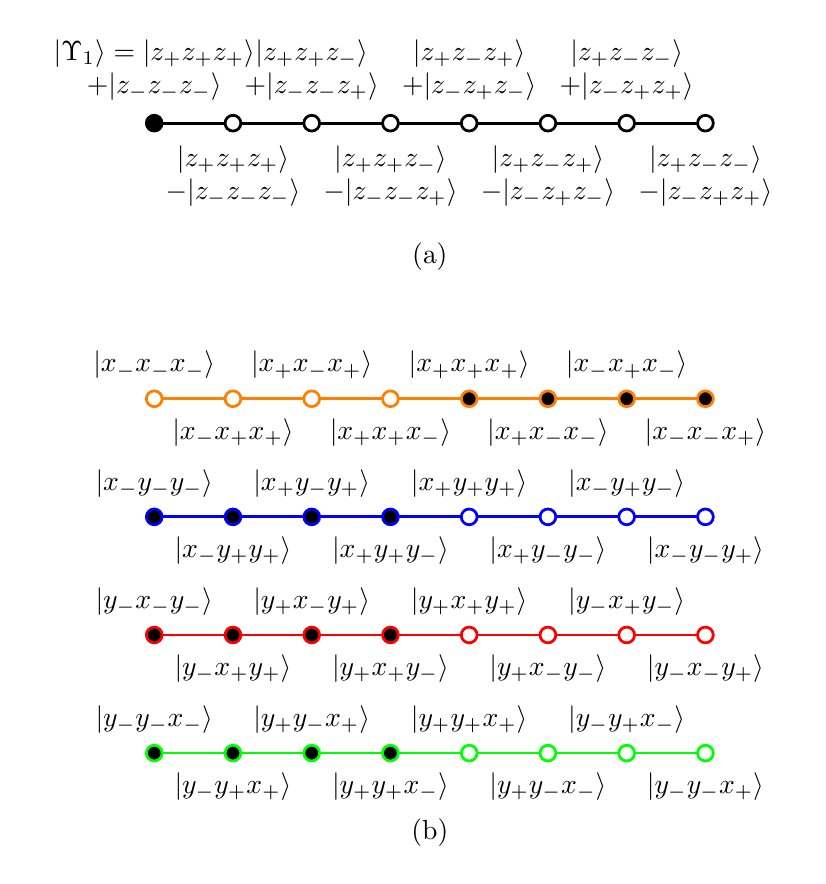
\begin{tikzpicture}  [scale=1]

\tikzstyle{every path}=[line width=1pt]

\newdimen\ms
\ms=0.1cm
\tikzstyle{s1}=[color=red,rectangle,inner sep=3.5]
\tikzstyle{c3}=[circle,inner sep={\ms/8},minimum size=4*\ms]
\tikzstyle{c2}=[circle,inner sep={\ms/8},minimum size=3*\ms]
\tikzstyle{c1}=[circle,inner sep={\ms/8},minimum size=2*\ms]
\tikzstyle{cs1}=[circle,inner sep={\ms/8},minimum size=1*\ms]

% Define positions of all observables

\coordinate (uuu) at (0,8);
\coordinate (uuv) at (1,8);
\coordinate (uvu) at (2,8);
\coordinate (uvv) at (3,8);
\coordinate (vuu) at (4,8);
\coordinate (vuv) at (5,8);
\coordinate (vvu) at (6,8);
\coordinate (vvv) at (7,8);

% draw contexts

\draw [color=black] (uuu) -- (vvv);

% draw atoms

\draw (uuu) coordinate[c1,fill=black, draw=black,label=above:{\begin{tabular}{c} $\vert \Upsilon_1 \rangle =\vert z_+z_+z_+ \rangle $\\$ + \vert z_-z_-z_- \rangle $\end{tabular}}];
\draw (uuv) coordinate[c1,fill=white, draw=black,label=below:{\begin{tabular}{c} $\vert z_+z_+z_+ \rangle $\\$ - \vert z_-z_-z_- \rangle $\end{tabular}}];
\draw (uvu) coordinate[c1,fill=white, draw=black,label=above:{\begin{tabular}{c} $\vert z_+z_+z_- \rangle $\\$ + \vert z_-z_-z_+ \rangle $\end{tabular}}];
\draw (uvv) coordinate[c1,fill=white, draw=black,label=below:{\begin{tabular}{c} $\vert z_+z_+z_- \rangle $\\$ - \vert z_-z_-z_+ \rangle $\end{tabular}}];
\draw (vuu) coordinate[c1,fill=white, draw=black,label=above:{\begin{tabular}{c} $\vert z_+z_-z_+ \rangle $\\$ + \vert z_-z_+z_- \rangle $\end{tabular}}];
\draw (vuv) coordinate[c1,fill=white, draw=black,label=below:{\begin{tabular}{c} $\vert z_+z_-z_+ \rangle $\\$ - \vert z_-z_+z_- \rangle $\end{tabular}}];
\draw (vvu) coordinate[c1,fill=white, draw=black,label=above:{\begin{tabular}{c} $\vert z_+z_-z_- \rangle $\\$ + \vert z_-z_+z_+ \rangle $\end{tabular}}];
\draw (vvv) coordinate[c1,fill=white, draw=black,label=below:{\begin{tabular}{c} $\vert z_+z_-z_- \rangle $\\$ - \vert z_-z_+z_+ \rangle $\end{tabular}}];

\coordinate (a) at (3.5,6);
\draw (a) coordinate[label=above:(a)];

% Define positions of all observables

% Define positions of all observables

\coordinate (ccu) at (0,4.5);
\coordinate (ccv) at (1,4.5);
\coordinate (cdu) at (2,4.5);
\coordinate (cdv) at (3,4.5);
\coordinate (dcu) at (4,4.5);
\coordinate (dcv) at (5,4.5);
\coordinate (ddu) at (6,4.5);
\coordinate (ddv) at (7,4.5);

\coordinate (cuc) at (0,3);
\coordinate (cvc) at (1,3);
\coordinate (cud) at (2,3);
\coordinate (cvd) at (3,3);
\coordinate (duc) at (4,3);
\coordinate (dvc) at (5,3);
\coordinate (dud) at (6,3);
\coordinate (dvd) at (7,3);

\coordinate (ucc) at (0,1.5);
\coordinate (vcc) at (1,1.5);
\coordinate (ucd) at (2,1.5);
\coordinate (vcd) at (3,1.5);
\coordinate (udc) at (4,1.5);
\coordinate (vdc) at (5,1.5);
\coordinate (udd) at (6,1.5);
\coordinate (vdd) at (7,1.5);

\coordinate (uuu) at (0,0);
\coordinate (uuv) at (1,0);
\coordinate (uvu) at (2,0);
\coordinate (uvv) at (3,0);
\coordinate (vuu) at (4,0);
\coordinate (vuv) at (5,0);
\coordinate (vvu) at (6,0);
\coordinate (vvv) at (7,0);

% draw contexts

\draw [color=orange] (ccu) -- (ddv);
\draw [color=blue] (cuc) -- (dvd);
\draw [color=red] (ucc) -- (vdd);
\draw [color=green] (uuu) -- (vvv);

% draw atoms


\draw (ccu) coordinate[c1,fill=white, draw=orange,label=above:$\vert x_-  x_-  x_- \rangle $];
\draw (ccv) coordinate[c1,fill=white, draw=orange,label=below:$\vert x_-  x_+  x_+ \rangle $];
\draw (cdu) coordinate[c1,fill=white, draw=orange,label=above:$\vert x_+  x_-  x_+ \rangle $];
\draw (cdv) coordinate[c1,fill=white, draw=orange,label=below:$\vert x_+  x_+  x_- \rangle $];
\draw (dcu) coordinate[c1,fill=black, draw=orange,label=above:$\vert x_+  x_+  x_+ \rangle $];
\draw (dcv) coordinate[c1,fill=black, draw=orange,label=below:$\vert x_+  x_-  x_- \rangle $];
\draw (ddu) coordinate[c1,fill=black, draw=orange,label=above:$\vert x_-  x_+  x_- \rangle $];
\draw (ddv) coordinate[c1,fill=black, draw=orange,label=below:$\vert x_-  x_-  x_+ \rangle $];

  \draw (cuc) coordinate[c1,fill=black, draw=blue,label=above:$\vert x_-  y_-  y_- \rangle $];
  \draw (cvc) coordinate[c1,fill=black, draw=blue,label=below:$\vert x_-  y_+  y_+ \rangle $];
  \draw (cud) coordinate[c1,fill=black, draw=blue,label=above:$\vert x_+  y_-  y_+ \rangle $];
  \draw (cvd) coordinate[c1,fill=black, draw=blue,label=below:$\vert x_+  y_+  y_- \rangle $];
  \draw (duc) coordinate[c1,fill=white, draw=blue,label=above:$\vert x_+  y_+  y_+ \rangle $];
  \draw (dvc) coordinate[c1,fill=white, draw=blue,label=below:$\vert x_+  y_-  y_- \rangle $];
  \draw (dud) coordinate[c1,fill=white, draw=blue,label=above:$\vert x_-  y_+  y_- \rangle $];
  \draw (dvd) coordinate[c1,fill=white, draw=blue,label=below:$\vert x_-  y_-  y_+ \rangle $];

   \draw (ucc) coordinate[c1,fill=black, draw=red,label=above:$\vert y_-  x_-  y_- \rangle $];
   \draw (vcc) coordinate[c1,fill=black, draw=red,label=below:$\vert y_-  x_+  y_+ \rangle $];
   \draw (ucd) coordinate[c1,fill=black, draw=red,label=above:$\vert y_+  x_-  y_+ \rangle $];
   \draw (vcd) coordinate[c1,fill=black, draw=red,label=below:$\vert y_+  x_+  y_- \rangle $];
   \draw (udc) coordinate[c1,fill=white, draw=red,label=above:$\vert y_+  x_+  y_+ \rangle $];
   \draw (vdc) coordinate[c1,fill=white, draw=red,label=below:$\vert y_+  x_-  y_- \rangle $];
   \draw (udd) coordinate[c1,fill=white, draw=red,label=above:$\vert y_-  x_+  y_- \rangle $];
   \draw (vdd) coordinate[c1,fill=white, draw=red,label=below:$\vert y_-  x_-  y_+ \rangle $];

 \draw (uuu) coordinate[c1,fill=black, draw=green,label=above:$\vert y_-  y_-  x_- \rangle $];
 \draw (uuv) coordinate[c1,fill=black, draw=green,label=below:$\vert y_-  y_+  x_+ \rangle $];
 \draw (uvu) coordinate[c1,fill=black, draw=green,label=above:$\vert y_+  y_-  x_+ \rangle $];
 \draw (uvv) coordinate[c1,fill=black, draw=green,label=below:$\vert y_+  y_+  x_- \rangle $];
 \draw (vuu) coordinate[c1,fill=white, draw=green,label=above:$\vert y_+  y_+  x_+ \rangle $];
 \draw (vuv) coordinate[c1,fill=white, draw=green,label=below:$\vert y_+  y_-  x_- \rangle $];
 \draw (vvu) coordinate[c1,fill=white, draw=green,label=above:$\vert y_-  y_+  x_- \rangle $];
 \draw (vvv) coordinate[c1,fill=white, draw=green,label=below:$\vert y_-  y_-  x_+ \rangle $];

\coordinate (b) at (3.5,-0.7);
\draw (b) coordinate[label=below:(b)];

\end{tikzpicture}
}
\end{center}
\caption{\label{2020-f-ghz-contextqm}
Hypergraphs representing  (a) GHZ states forming a single quantum mechanical GHZ state context
represented by the GHZ basis of the eigenstates of $\sigma_z \sigma_z \sigma_z$,
and (b) the four nonintertwining GHZ contexts in the four bases of the eigenstates of
$\sigma_y \sigma_y \sigma_x$, $\sigma_y \sigma_x \sigma_y$, $\sigma_x \sigma_y \sigma_y$,  and $\sigma_x \sigma_x \sigma_x$
with eight atoms each.
Filled circles indicate states ``allowed'' by---that is, are equal to or
occur in the coherent superposition of---the original GHZ game state
$\vert \Upsilon_1 \rangle = \vert z_+z_+z_+ \rangle  + \vert z_-z_-z_- \rangle$
as enumerated in Eqs.~(\ref{2020-ghz-evsisjsk}) and~(\ref{2020-ex-rew-ghz}),
yielding a discord with classical means and predictions.
A comparison of the classical $\{x,x,x\}$ context drawn on top of Figure~\ref{2020-f-ghz-contextconf}(b)
yields an ``inverted'' situation:
the ``allowed'' states are classically ``disallowed'', and vice versa.
}
\end{figure}

Another, algebraic, way of perceiving this is in terms of the mutual commutativity of
the four operators
$\sigma_y \sigma_y \sigma_x$, $\sigma_y \sigma_x \sigma_y$, $\sigma_x \sigma_y \sigma_y$,  and $\sigma_x \sigma_x \sigma_x$
in Eq.~(\ref{2020-ghz-sigmas-contextop}), which thus can be written as real-valued functions of
a maximal operator~\cite[\S~84, p.~171,172]{halmos-vs}
\begin{equation}
\textsf{\textbf{R}} = \sum_{i=1}^8 \lambda_i \vert \Upsilon_i \rangle \langle  \Upsilon_i \vert ,
\label{2020-ghz-mo}
\end{equation}
with mutually different $\lambda_i$ and $\vert \Upsilon_i \rangle$ defined in Eq.~(\ref{2020-ghz-evsisjsk}).
As can be readily read off from Table~\ref{2020-hardy-t-eveeva}, and with
$f_{yyx}(\textsf{\textbf{R}})=\sigma_y \sigma_y \sigma_x$,
$f_{yxy}(\textsf{\textbf{R}})=\sigma_y \sigma_x \sigma_y$,
$f_{xyy}(\textsf{\textbf{R}})=\sigma_x \sigma_y \sigma_y$,  and
$f_{xxx}(\textsf{\textbf{R}})=\sigma_x \sigma_x \sigma_x$
these four functions need to obey
$
-f_{yyx}(\lambda_1)=
f_{yyx}(\lambda_2)=
-f_{yyx}(\lambda_3)=
f_{yyx}(\lambda_4)=
f_{yyx}(\lambda_5)=
-f_{yyx}(\lambda_6)=
f_{yyx}(\lambda_7)=
-f_{yyx}(\lambda_8)=
%1$,
%$
-f_{yxy}(\lambda_1)=
f_{yxy}(\lambda_2)=
f_{yxy}(\lambda_3)=
-f_{yxy}(\lambda_4)=
-f_{yxy}(\lambda_5)=
f_{yxy}(\lambda_6)=
f_{yxy}(\lambda_7)=
-f_{yxy}(\lambda_8)=
%1$,
%$
-f_{xyy}(\lambda_1)=
f_{xyy}(\lambda_2)=
f_{xyy}(\lambda_3)=
-f_{xyy}(\lambda_4)=
f_{xyy}(\lambda_5)=
-f_{xyy}(\lambda_6)=
-f_{xyy}(\lambda_7)=
f_{xyy}(\lambda_8)=
%1$,
%$
f_{xxx}(\lambda_1)=
-f_{xxx}(\lambda_2)=
f_{xxx}(\lambda_3)=
-f_{xxx}(\lambda_4)=
f_{xxx}(\lambda_5)=
-f_{xxx}(\lambda_6)=
f_{xxx}(\lambda_7)=
-f_{xxx}(\lambda_8)=
1$.


\subsection{Verification of the original quantum GHZ game}

Let us review our solution to the original GHZ game.
It can be won with
quantum resources from the GHZ basis
enumerated in (\ref{2020-ghz-context}) and (\ref{2020-ghz-evsisjsk}).
If the prisoners share a particular quantum state representable by Eq.~(\ref{2020-ghz-psiGHZ}), namely
$\vert \Upsilon_1 \rangle = \frac{1}{\sqrt{2}}
\left(
\vert {z_+}{z_+}{z_+} \rangle +
\vert {z_-}{z_-}{z_-} \rangle
\right)$
prepared in one direction, say $z$,
prior to being separated, this goal can be achieved.
Because the prisoners measure, on their respective sides and constituents particles
(the share includes three constituents because it is a three-partite state),
 $\vert \Upsilon_1 \rangle$ either in the $x$ basis
$\vert x_\pm \rangle  = \frac{1}{\sqrt{2}}
\left(
\vert {z_+} \rangle \pm
\vert {z_-} \rangle
\right)  = \frac{1}{\sqrt{2}}
\begin{pmatrix}
1,\pm 1
\end{pmatrix}
$
[conversely,
$\vert {z_\pm} \rangle  = \frac{1}{\sqrt{2}}
\left(
\vert x_+ \rangle \pm
\vert x_- \rangle
\right)
${\large]}
whenever their slip says ``$x$'',
or   in the $y$ basis
$\vert y_\pm \rangle  = \frac{1}{\sqrt{2}}
\left(
\vert {z_+} \rangle \pm
i
\vert {z_-} \rangle
\right) = \frac{1}{\sqrt{2}}
\begin{pmatrix}
1,\pm i
\end{pmatrix}
$
[conversely,
$\vert {z_+} \rangle  = \frac{1}{\sqrt{2}}
\left(
\vert y_+ \rangle +
\vert y_- \rangle
\right)$
and $\vert {z_-} \rangle  = -\frac{i}{\sqrt{2}}
\left(
\vert y_+ \rangle +
\vert y_- \rangle
\right)
${\large]}
whenever their slip says ``$y$''.

That this goal can be perfectly---ideally at all instances and configurations---reached
can be demonstrated by rewriting the
GHZ state $\vert \Upsilon_1 \rangle $
in terms of the basis vectors of the four configurations or contexts,
one of which is singled out (but not disclosed to the prisoners) by the prison ward
[see also the filled states in the contexts depicted in Figure~\ref{2020-f-ghz-contextqm}(b)]:
\begin{equation}
\begin{aligned}
\vert \Upsilon_1 \rangle
&=  \frac{1}{2}
%2 (x1p x2m x3m + x1m x2p x3m + x1m x2m x3p + x1p x2p x3p)
\left(
\vert x_+  x_+  x_+  \rangle +
\vert x_+  x_-  x_-  \rangle +
\vert x_-  x_+  x_-  \rangle +
\vert x_-  x_-  x_+  \rangle
\right)  \\
&=  \frac{1}{2}
%2 (x1m y2m y3m                + x1p y2p y3m + x1p y2m y3p + x1m y2p y3p)
\left(
\vert x_-  y_-  y_-  \rangle +
\vert x_-  y_+  y_+  \rangle +
\vert x_+  y_-  y_+  \rangle +
\vert x_+  y_+  y_-  \rangle
\right)  \\
&=  \frac{1}{2}
%2 (x2m y1m y3m                + x2p y1p y3m + x2p y1m y3p + x2m y1p y3p)
\left(
\vert y_-  x_-  y_-  \rangle +
\vert y_-  x_+  y_+  \rangle +
\vert y_+  x_-  y_+  \rangle +
\vert y_+  x_+  y_-  \rangle
\right)  \\
&=  \frac{1}{2}
\left(
%2 (x3m y1m y2m                + x3p y1p y2m + x3p y1m y2p + x3m y1p y2p)
\vert  y_-  y_-  x_-  \rangle +
\vert  y_-  y_+  x_+  \rangle +
\vert  y_+  y_-  x_+  \rangle +
\vert  y_+  y_+  x_-  \rangle
\right)
.
\end{aligned}
\label{2020-ex-rew-ghz}
\end{equation}
For every individual experimental run,
the share ``produces'' or ``selects'' one of the four outcomes from the coherent superpositions.

Note that there is a ``hidden cost''  in this game:
to make sure that the quantum $xxx$ realization conforms with the other three choices  $xyy$, $yxy$, and $yyx$
of the ward, one needs to either believe in this counterfactual supposition
or make additional experiments to verify the latter three.
But more experimental runs are added which are ``hidden'' away by acknowledging
that first checks of $xyy$, $yxy$, and $yyx$ have to be performed; and, as stated in Ref.~\cite[p.~517]{panbdwz},
{\it ``if the results obtained are in agreement with the predictions for a GHZ
state, then for an $xxx$ experiment, our expectations
using a local-realist theory are exactly the opposite of our expectations
using quantum physics.''}
Confidence about whether one is dealing with a GHZ state $\vert \Upsilon_1 \rangle $
(by checking the outcomes of the $xyy$, $yxy$, and $yyx$ and finally $xxx$ configurations)
requires additional experimental runs.

The GHZ scenario can be interpreted as some nonlocal form of Hardy-type
true-implies-true scenario with ``maximal aperture'' $\frac{\pi}{2}$.
This can, for example, be achieved by
serial composition~\cite{svozil-2018-whycontexts} of such true-implies-true gadgets~\cite{2018-minimalYIYS};
a procedure already performed by Kochen and Specker~\cite{kochen1}, as they move from $\Gamma_1$ to $\Gamma_2$.




\section{Generalization of GHZ games}

Table~\ref{2020-hardy-t-eveeva} enumerates the eight variations of GHZ games
with viable winning strategies for the prisoners.
Those strategies are based on modified GHZ states as assets.
By the earlier parity argument, it is again impossible for the prisoners employing classical means
to win for all such paper slip configurations the ward might issue.
These variations can be translated into experimental protocols analogous to the ones executed in Refs.~\cite{PhysRevLett.82.1345,panbdwz}.

Suppose, for the sake of an example, the prison ward requires the respective products of
$xyy$, $yxy$, and $yyx$  to turn out positive and $xxx$ to turn out negative.
This can be won by the prisoners with a $\vert \Upsilon_2 \rangle = \frac{1}{\sqrt{2}}\left( \vert z_+z_+z_+ \rangle  - \vert z_-z_-z_- \rangle \right) $ share.

Or suppose, for the sake of another example, the prison ward requires the respective products of
$xyy$  to turn out positive and $yyx$, $yxy$, and $xxx$ to turn out negative.
The prisoners can win this with a $\vert \Upsilon_8 \rangle = \frac{1}{\sqrt{2}}\left( \vert z_+z_-z_- \rangle  - \vert z_-z_+z_+ \rangle \right) $ share.
The respective game components are
\begin{equation}
\begin{aligned}
\vert \Upsilon_8 \rangle
&=  -\frac{1}{2}
\left(
%-2 x1p (x2p x3m + x2m x3p) + 2 x1m (x2m x3m + x2p x3p)
\vert x_+x_+x_- \rangle +
\vert x_+x_-x_+ \rangle -
\vert x_-x_-x_- \rangle -
\vert x_-x_+x_+ \rangle
\right)  \\
&=  \frac{1}{2}
\left(
%2 x1m (y2p y3m + y2m y3p) - 2 x1p (y2m y3m + y2p y3p)
\vert x_-y_+y_- \rangle +
\vert x_-y_-y_+ \rangle -
\vert x_+y_-y_- \rangle -
\vert x_+y_+y_+ \rangle
\right)  \\
&=  -\frac{i}{2}
\left(
%-2 I (x2m y1m y3m - x2p y1p y3m + x2p y1m y3p - x2m y1p y3p)
\vert y_-x_-y_- \rangle -
\vert y_+x_+y_- \rangle +
\vert y_-x_+y_+ \rangle -
\vert y_+x_-y_+ \rangle
\right)  \\
&=  -\frac{i}{2}
\left(
% -2 I (x3m y1m y2m - x3p y1p y2m + x3p y1m y2p - x3m y1p y2p)
\vert y_-y_-x_- \rangle -
\vert y_+y_-x_+ \rangle +
\vert y_-y_+x_+ \rangle -
\vert y_+y_+x_- \rangle
\right)
.
\end{aligned}
\label{2020-ex-rew-ghz8}
\end{equation}

Because of symmetry, we may expect that not much changes regarding gambling if we permute $\sigma_1 \leftrightarrow \sigma_2$. Here we need to form a
modified GHZ basis serving as eigenstates, with the first ``$1$'' component of the vectors of the original GHZ basis substituted by the imaginary unit ``$i$''.
With those eigenstates Table~\ref{2020-hardy-t-eveeva} is reproduced.


\section{Games that can be won by classical but not by quantum GHZ means}
\label{2020-ghz-gtcbwbcbnbqm}

It should also be mentioned what the prisoners cannot achieve with GHZ type quantum resources.
Table~\ref{2020-hardy-t-eveeva} does not allow a
perfect winning strategy for the aforementioned games in which the ward requests from the prisoners to produce only positive or negative outcomes.
They can win these games with the classical strategies or shares mentioned earlier.
Table~\ref{2020-hardy-t-eveevac} enumerates the configurations
and some of the (eight per configuration) classical winning strategies.

\begin{table}[t]%%[H] add [H] placement to break table across pages
 \begin{center}
 \caption{Enumeration of the eight configurations that cannot be won with quantum GHZ type shares, and one (of the eight per configuration) classical winning strategies.
\label{2020-hardy-t-eveevac}}
\begin{ruledtabular}
 \begin{tabular}{ c c c c c c c c c c c c }
%\ruledtabular
$1^\text{st}$ prisoner&$2^\text{nd}$ prisoner&$3^\text{rd}$ prisoner&    $yyx$ & $yxy$ &  $xyy$  & $xxx$
\\
\hline
$x=-1$ & $x=-1$ & $x=-1$&  {\Large -} & {\Large -} &  {\Large -} & {\Large -}\\
$y=-1$ & $y=-1$ & $y= -1$\\
$x=-1$ & $x=-1$ & $x=+1$&   {\Large -} & {\Large -} &  {\Large +} & {\Large +}\\
$y=-1$ & $y=+1$ & $y= -1$\\
$x=-1$ & $x=-1$ & $x=-1$&   {\Large -} & {\Large +} &  {\Large +} & {\Large -}\\
$y=-1$ & $y=-1$ & $y= +1$\\
$x=-1$ & $x=-1$ & $x=+1$&   {\Large -} & {\Large +} &  {\Large -} & {\Large +}\\
$y=-1$ & $y=+1$ & $y= +1$\\
$x=-1$ & $x=-1$ & $x=-1$&   {\Large +} & {\Large -} &  {\Large +} & {\Large -}\\
$y=-1$ & $y=+1$ & $y= -1$\\
$x=-1$ & $x=-1$ & $x=+1$&   {\Large +} & {\Large -} &  {\Large -} & {\Large +}\\
$y=-1$ & $y=-1$ & $y= -1$\\
$x=-1$ & $x=-1$ & $x=-1$&   {\Large +} & {\Large +} &  {\Large -} & {\Large -}\\
$y=-1$ & $y=+1$ & $y= +1$\\
$x=+1$&$x=+1$&$x=+1$& {\Large +} & {\Large +} &  {\Large +} & {\Large +}\\
$y=+ 1$ & $y=+1$ & $y= + 1$
%\\ \ruledtabular
\end{tabular}
\end{ruledtabular}
 \end{center}
 \end{table}



\section{Classical contextuality or context dependence}

An examination of the subgraph of the GHZ logic hypergraph, depicted in Figure~\ref{2020-f-ghz-contextqm}(b) ``covered'' by $\vert \Upsilon_1 \rangle$
shows that this (sub)logic has a separating set of $8^4$ admissible two-valued states
satisfying completeness (every context contains a red or 1 value) and exclusivity (every context contains only one red or 1 value, all other vertices are green or 0 value).

For the sake of demonstration, this propositional structure can further be
``tightened'' by introducing four additional ``vertical'' and four additional ``diagonal'' contexts as depicted in Figure~\ref{2020-f-ghz-contextpl}.
The resulting tightened GHZ (sub)logic comprising 12 contexts supports eight two-valued states which are separating any two different propositions.
They are enumerated in Figure~\ref{2020-f-ghz-contextghz2vs}.
(In this presentation the two-valued states appear like $0-1$ entries in permutation matrices.)
Consequently, this configuration has a classical
representation by a partition logic $\{1,2,\ldots ,8\}$ of eight elements, as drawn in Figure~\ref{2020-f-ghz-contextpl}.

\begin{figure}[htb!]%[H]
\begin{center}
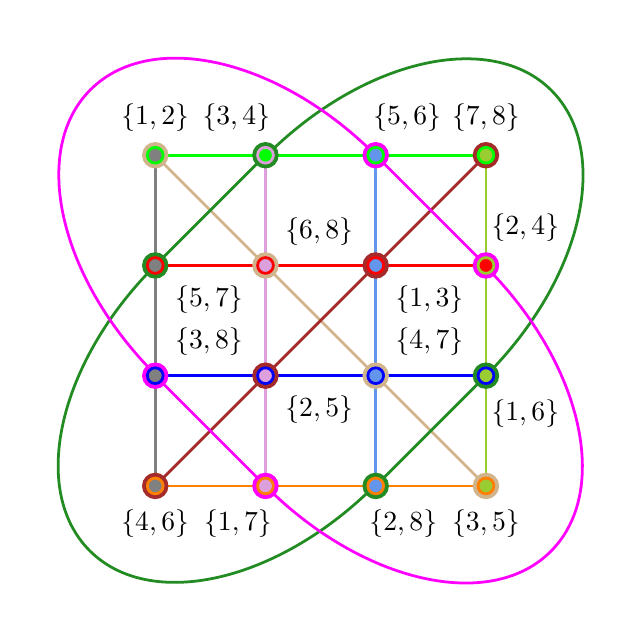
\begin{tikzpicture}  [scale=0.7]

\tikzstyle{every path}=[line width=1pt]

\newdimen\ms
\ms=0.1cm
\tikzstyle{s1}=[color=red,rectangle,inner sep=3.5]
\tikzstyle{c3}=[circle,inner sep={\ms/8},minimum size=4*\ms]
\tikzstyle{c2}=[circle,inner sep={\ms/8},minimum size=3*\ms]
\tikzstyle{c1}=[circle,inner sep={\ms/8},minimum size=2*\ms]
\tikzstyle{cs1}=[circle,inner sep={\ms/8},minimum size=1*\ms]


% Define positions of all observables

\coordinate (uuu) at ( 0,6);
\coordinate (uuv) at ( 2,6);
\coordinate (uvu) at ( 4,6);
\coordinate (uvv) at ( 6,6);
\coordinate (vuu) at ( 8,6);
\coordinate (vuv) at (10,6);
\coordinate (vvu) at (12,6);
\coordinate (vvv) at (14,6);


\coordinate (ucc) at ( 0,4);
\coordinate (vcc) at ( 2,4);
\coordinate (ucd) at ( 4,4);
\coordinate (vcd) at ( 6,4);
\coordinate (udc) at ( 8,4);
\coordinate (vdc) at (10,4);
\coordinate (udd) at (12,4);
\coordinate (vdd) at (14,4);

\coordinate (cuc) at ( 0,2);
\coordinate (cvc) at ( 2,2);
\coordinate (cud) at ( 4,2);
\coordinate (cvd) at ( 6,2);
\coordinate (duc) at ( 8,2);
\coordinate (dvc) at (10,2);
\coordinate (dud) at (12,2);
\coordinate (dvd) at (14,2);

\coordinate (ccu) at ( 0,0);
\coordinate (ccv) at ( 2,0);
\coordinate (cdu) at ( 4,0);
\coordinate (cdv) at ( 6,0);
\coordinate (dcu) at ( 8,0);
\coordinate (dcv) at (10,0);
\coordinate (ddu) at (12,0);
\coordinate (ddv) at (14,0);




% draw contexts

\draw [color=orange] (ccu) -- (cdv);
\draw [color=blue] (cuc) -- (cvd);
\draw [color=red] (ucc) -- (vcd);
\draw [color=green] (uuu) -- (uvv);

\draw [color=Gray] (uuu) -- (ccu);
\draw [color=Plum] (uuv) -- (ccv);
\draw [color=CornflowerBlue] (uvu) -- (cdu);
\draw [color=YellowGreen] (uvv) -- (cdv);


\draw [color=Tan] (uuu) -- (cdv);
\draw [color=Brown] (uvv) -- (ccu);


\draw [color=ForestGreen] (uuv) -- (ucc);
\draw [color=ForestGreen](cdu) -- (cvd);
\draw [rotate=225,color=ForestGreen] (cvd) arc (90:270:4.5 and 2.82);
\draw[rotate=45,color=ForestGreen] (ucc) arc (90:270:4.5 and 2.82);

\draw [color=Magenta] (cuc) -- (ccv);
\draw [color=Magenta] (uvu) -- (vcd);
\draw[rotate=315,color=Magenta] (uvu) arc (90:270:4.5 and 2.82);
\draw[rotate=135,color=Magenta] (ccv) arc (90:270:4.5 and 2.82);


%draw atoms




 \draw (uuu) coordinate[c2,fill=Tan,draw=Tan,label=above:{$\{1,2\}$}];
 \draw (uuu) coordinate[c1,fill=Gray,draw=green];
 \draw (uuv) coordinate[c2,fill=ForestGreen,draw=ForestGreen,label={[xshift=-3.7mm]90:$\{3,4\}$}];
 \draw (uuv) coordinate[c1,fill=green,draw=Plum];
 \draw (uvu) coordinate[c2,fill=Magenta,draw=Magenta,label={[xshift=+4mm]90:$\{5,6\}$}];
 \draw (uvu) coordinate[c1,fill=CornflowerBlue,draw=green];
 \draw (uvv) coordinate[c2,fill=Brown,draw=Brown,label=above:{$\{7,8\}$}];
 \draw (uvv) coordinate[c1,fill=YellowGreen,draw=green];


  % \draw (ucc) coordinate[c2,fill=ForestGreen,draw=ForestGreen,label={[xshift=-7.5mm,distance=0mm]90:$\{x_-  y_-  y_-\}$}];
   \draw (ucc) coordinate[c2,fill=ForestGreen,draw=ForestGreen,label=below right:{$\{5,7\}$}];
   \draw (ucc) coordinate[c1,fill=Gray,draw=red];
   \draw (vcc) coordinate[c2,fill=Tan,draw=Tan,label=above right:{$\{6,8\}$}];
   \draw (vcc) coordinate[c1,fill=Plum,draw=red];
   \draw (ucd) coordinate[c2,fill=Brown,draw=Brown,label=below right:{$\{1,3\}$}];
   \draw (ucd) coordinate[c1,fill=CornflowerBlue,draw=red];
  % \draw (vcd) coordinate[c2,fill=Magenta,draw=Magenta,label=above right:{$\{x_+  y_+  y_-\}$}];
   \draw (vcd) coordinate[c2,fill=Magenta,draw=Magenta,label={[xshift=+5mm,distance=10mm]90:$\{2,4\}$}];
   \draw (vcd) coordinate[c1,fill=red,draw=YellowGreen];

  \draw (cuc) coordinate[c2,fill=Magenta,draw=Magenta,label=above right:{$\{3,8\}$}];
  \draw (cuc) coordinate[c1,fill=Gray,draw=blue];
  \draw (cvc) coordinate[c2,fill=Brown,draw=Brown,label=below right:{$\{2,5\}$}];
  \draw (cvc) coordinate[c1,fill=Plum,draw=blue];
  \draw (cud) coordinate[c2,fill=Tan,draw=Tan,label=above right:{$\{4,7\}$}];
  \draw (cud) coordinate[c1,fill=CornflowerBlue,draw=blue];
  \draw (cvd) coordinate[c2,fill=ForestGreen,draw=ForestGreen,label={[xshift=+5mm,distance=10mm]270:$\{1,6\}$}];
  \draw (cvd) coordinate[c1,fill=YellowGreen,draw=blue];

\draw (ccu) coordinate[c2,fill=Brown,draw=Brown,label=below:{$\{4,6\}$}];
\draw (ccu) coordinate[c1,fill=Gray,draw=orange];
\draw (ccv) coordinate[c2,fill=Magenta,draw=Magenta,label={[xshift=-3.5mm]270:$\{1,7\}$}];
\draw (ccv) coordinate[c1,fill=Plum,draw=orange];
\draw (cdu) coordinate[c2,fill=ForestGreen,draw=ForestGreen,label={[xshift=+3.5mm]270:$\{2,8\}$}];
\draw (cdu) coordinate[c1,fill=CornflowerBlue,draw=orange];
\draw (cdv) coordinate[c2,fill=Tan,draw=Tan,label=below:{$\{3,5\}$}];
\draw (cdv) coordinate[c1,fill=YellowGreen,draw=orange];



\end{tikzpicture}
\end{center}
\caption{\label{2020-f-ghz-contextpl}
Hypergraphs representing 12 tightly intertwined ``tightened'' GHZ contexts in a partition logic representation.
}
\end{figure}

\begin{figure}[htb!]%[H]
\begin{center}
\begin{tabular}{ c c }
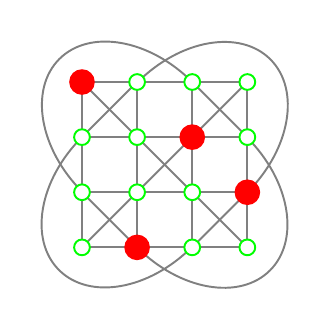
\begin{tikzpicture}  [scale=0.35]

\tikzstyle{every path}=[line width=0.7pt]

\newdimen\ms
\ms=0.1cm
\tikzstyle{s1}=[color=red,rectangle,inner sep=3.5]
\tikzstyle{c3}=[circle,inner sep={\ms/8},minimum size=4*\ms]
\tikzstyle{c2}=[circle,inner sep={\ms/8},minimum size=3*\ms]
\tikzstyle{c1}=[circle,inner sep={\ms/8},minimum size=2*\ms]
\tikzstyle{cs1}=[circle,inner sep={\ms/8},minimum size=1*\ms]

% Define positions of all observables

\coordinate (uuu) at ( 0,6);
\coordinate (uuv) at ( 2,6);
\coordinate (uvu) at ( 4,6);
\coordinate (uvv) at ( 6,6);
\coordinate (vuu) at ( 8,6);
\coordinate (vuv) at (10,6);
\coordinate (vvu) at (12,6);
\coordinate (vvv) at (14,6);

\coordinate (ucc) at ( 0,4);
\coordinate (vcc) at ( 2,4);
\coordinate (ucd) at ( 4,4);
\coordinate (vcd) at ( 6,4);
\coordinate (udc) at ( 8,4);
\coordinate (vdc) at (10,4);
\coordinate (udd) at (12,4);
\coordinate (vdd) at (14,4);

\coordinate (cuc) at ( 0,2);
\coordinate (cvc) at ( 2,2);
\coordinate (cud) at ( 4,2);
\coordinate (cvd) at ( 6,2);
\coordinate (duc) at ( 8,2);
\coordinate (dvc) at (10,2);
\coordinate (dud) at (12,2);
\coordinate (dvd) at (14,2);

\coordinate (ccu) at ( 0,0);
\coordinate (ccv) at ( 2,0);
\coordinate (cdu) at ( 4,0);
\coordinate (cdv) at ( 6,0);
\coordinate (dcu) at ( 8,0);
\coordinate (dcv) at (10,0);
\coordinate (ddu) at (12,0);
\coordinate (ddv) at (14,0);

% draw contexts

\draw [color=Gray] (ccu) -- (cdv);
\draw [color=Gray] (cuc) -- (cvd);
\draw [color=Gray] (ucc) -- (vcd);
\draw [color=Gray] (uuu) -- (uvv);

\draw [color=Gray] (uuu) -- (ccu);
\draw [color=Gray] (uuv) -- (ccv);
\draw [color=Gray] (uvu) -- (cdu);
\draw [color=Gray] (uvv) -- (cdv);

\draw [color=Gray] (uuu) -- (cdv);
\draw [color=Gray] (uvv) -- (ccu);

\draw [color=Gray] (uuv) -- (ucc);
\draw [color=Gray](cdu) -- (cvd);
\draw [rotate=225,color=Gray] (cvd) arc (90:270:4 and 2.82);
\draw[rotate=45,color=Gray] (ucc) arc (90:270:4 and 2.82);

\draw [color=Gray] (cuc) -- (ccv);
\draw [color=Gray] (uvu) -- (vcd);
\draw[rotate=315,color=Gray] (uvu) arc (90:270:4 and 2.82);
\draw[rotate=135,color=Gray] (ccv) arc (90:270:4 and 2.82);

%draw atoms

\draw (uuu) coordinate[c2,fill=red,draw=red];
\draw (uuv) coordinate[c1,fill=white,draw=green];
\draw (uvu) coordinate[c1,fill=white,draw=green];
\draw (uvv) coordinate[c1,fill=white,draw=green];


\draw (ucc) coordinate[c1,fill=white,draw=green];
\draw (vcc) coordinate[c1,fill=white,draw=green];
\draw (ucd) coordinate[c2,fill=red,draw=red];
\draw (vcd) coordinate[c1,fill=white,draw=green];

\draw (cuc) coordinate[c1,fill=white,draw=green];
\draw (cvc) coordinate[c1,fill=white,draw=green];
\draw (cud) coordinate[c1,fill=white,draw=green];
\draw (cvd) coordinate[c2,fill=red,draw=red];

\draw (ccu) coordinate[c1,fill=white,draw=green];
\draw (ccv) coordinate[c2,fill=red,draw=red];
\draw (cdu) coordinate[c1,fill=white,draw=green];
\draw (cdv) coordinate[c1,fill=white,draw=green];

\end{tikzpicture}
%%%%%%%%%%%%% 2
&
%
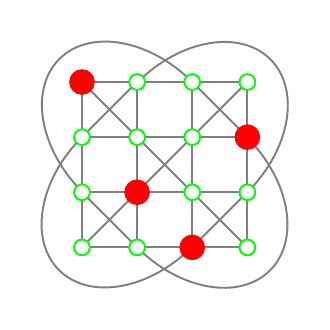
\begin{tikzpicture}  [scale=0.35]

\tikzstyle{every path}=[line width=0.7pt]

\newdimen\ms
\ms=0.1cm
\tikzstyle{s1}=[color=red,rectangle,inner sep=3.5]
\tikzstyle{c3}=[circle,inner sep={\ms/8},minimum size=4*\ms]
\tikzstyle{c2}=[circle,inner sep={\ms/8},minimum size=3*\ms]
\tikzstyle{c1}=[circle,inner sep={\ms/8},minimum size=2*\ms]
\tikzstyle{cs1}=[circle,inner sep={\ms/8},minimum size=1*\ms]

% Define positions of all observables

\coordinate (uuu) at ( 0,6);
\coordinate (uuv) at ( 2,6);
\coordinate (uvu) at ( 4,6);
\coordinate (uvv) at ( 6,6);
\coordinate (vuu) at ( 8,6);
\coordinate (vuv) at (10,6);
\coordinate (vvu) at (12,6);
\coordinate (vvv) at (14,6);

\coordinate (ucc) at ( 0,4);
\coordinate (vcc) at ( 2,4);
\coordinate (ucd) at ( 4,4);
\coordinate (vcd) at ( 6,4);
\coordinate (udc) at ( 8,4);
\coordinate (vdc) at (10,4);
\coordinate (udd) at (12,4);
\coordinate (vdd) at (14,4);

\coordinate (cuc) at ( 0,2);
\coordinate (cvc) at ( 2,2);
\coordinate (cud) at ( 4,2);
\coordinate (cvd) at ( 6,2);
\coordinate (duc) at ( 8,2);
\coordinate (dvc) at (10,2);
\coordinate (dud) at (12,2);
\coordinate (dvd) at (14,2);

\coordinate (ccu) at ( 0,0);
\coordinate (ccv) at ( 2,0);
\coordinate (cdu) at ( 4,0);
\coordinate (cdv) at ( 6,0);
\coordinate (dcu) at ( 8,0);
\coordinate (dcv) at (10,0);
\coordinate (ddu) at (12,0);
\coordinate (ddv) at (14,0);

% draw contexts

\draw [color=Gray] (ccu) -- (cdv);
\draw [color=Gray] (cuc) -- (cvd);
\draw [color=Gray] (ucc) -- (vcd);
\draw [color=Gray] (uuu) -- (uvv);

\draw [color=Gray] (uuu) -- (ccu);
\draw [color=Gray] (uuv) -- (ccv);
\draw [color=Gray] (uvu) -- (cdu);
\draw [color=Gray] (uvv) -- (cdv);

\draw [color=Gray] (uuu) -- (cdv);
\draw [color=Gray] (uvv) -- (ccu);

\draw [color=Gray] (uuv) -- (ucc);
\draw [color=Gray](cdu) -- (cvd);
\draw [rotate=225,color=Gray] (cvd) arc (90:270:4 and 2.82);
\draw[rotate=45,color=Gray] (ucc) arc (90:270:4 and 2.82);

\draw [color=Gray] (cuc) -- (ccv);
\draw [color=Gray] (uvu) -- (vcd);
\draw[rotate=315,color=Gray] (uvu) arc (90:270:4 and 2.82);
\draw[rotate=135,color=Gray] (ccv) arc (90:270:4 and 2.82);

%draw atoms

\draw (uuu) coordinate[c2,fill=red,draw=red];
\draw (uuv) coordinate[c1,fill=white,draw=green];
\draw (uvu) coordinate[c1,fill=white,draw=green];
\draw (uvv) coordinate[c1,fill=white,draw=green];


\draw (ucc) coordinate[c1,fill=white,draw=green];
\draw (vcc) coordinate[c1,fill=white,draw=green];
\draw (ucd) coordinate[c1,fill=white,draw=green];
\draw (vcd) coordinate[c2,fill=red,draw=red];

\draw (cuc) coordinate[c1,fill=white,draw=green];
\draw (cvc) coordinate[c2,fill=red,draw=red];
\draw (cud) coordinate[c1,fill=white,draw=green];
\draw (cvd) coordinate[c1,fill=white,draw=green];

\draw (ccu) coordinate[c1,fill=white,draw=green];
\draw (ccv) coordinate[c1,fill=white,draw=green];
\draw (cdu) coordinate[c2,fill=red,draw=red];
\draw (cdv) coordinate[c1,fill=white,draw=green];

\end{tikzpicture}
%
\\
%%%%%%%%%%%%%% 3
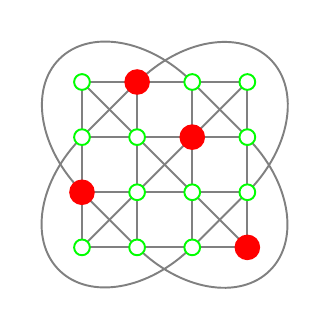
\begin{tikzpicture}  [scale=0.35]

\tikzstyle{every path}=[line width=0.7pt]

\newdimen\ms
\ms=0.1cm
\tikzstyle{s1}=[color=red,rectangle,inner sep=3.5]
\tikzstyle{c3}=[circle,inner sep={\ms/8},minimum size=4*\ms]
\tikzstyle{c2}=[circle,inner sep={\ms/8},minimum size=3*\ms]
\tikzstyle{c1}=[circle,inner sep={\ms/8},minimum size=2*\ms]
\tikzstyle{cs1}=[circle,inner sep={\ms/8},minimum size=1*\ms]

% Define positions of all observables

\coordinate (uuu) at ( 0,6);
\coordinate (uuv) at ( 2,6);
\coordinate (uvu) at ( 4,6);
\coordinate (uvv) at ( 6,6);
\coordinate (vuu) at ( 8,6);
\coordinate (vuv) at (10,6);
\coordinate (vvu) at (12,6);
\coordinate (vvv) at (14,6);

\coordinate (ucc) at ( 0,4);
\coordinate (vcc) at ( 2,4);
\coordinate (ucd) at ( 4,4);
\coordinate (vcd) at ( 6,4);
\coordinate (udc) at ( 8,4);
\coordinate (vdc) at (10,4);
\coordinate (udd) at (12,4);
\coordinate (vdd) at (14,4);

\coordinate (cuc) at ( 0,2);
\coordinate (cvc) at ( 2,2);
\coordinate (cud) at ( 4,2);
\coordinate (cvd) at ( 6,2);
\coordinate (duc) at ( 8,2);
\coordinate (dvc) at (10,2);
\coordinate (dud) at (12,2);
\coordinate (dvd) at (14,2);

\coordinate (ccu) at ( 0,0);
\coordinate (ccv) at ( 2,0);
\coordinate (cdu) at ( 4,0);
\coordinate (cdv) at ( 6,0);
\coordinate (dcu) at ( 8,0);
\coordinate (dcv) at (10,0);
\coordinate (ddu) at (12,0);
\coordinate (ddv) at (14,0);

% draw contexts

\draw [color=Gray] (ccu) -- (cdv);
\draw [color=Gray] (cuc) -- (cvd);
\draw [color=Gray] (ucc) -- (vcd);
\draw [color=Gray] (uuu) -- (uvv);

\draw [color=Gray] (uuu) -- (ccu);
\draw [color=Gray] (uuv) -- (ccv);
\draw [color=Gray] (uvu) -- (cdu);
\draw [color=Gray] (uvv) -- (cdv);

\draw [color=Gray] (uuu) -- (cdv);
\draw [color=Gray] (uvv) -- (ccu);

\draw [color=Gray] (uuv) -- (ucc);
\draw [color=Gray](cdu) -- (cvd);
\draw [rotate=225,color=Gray] (cvd) arc (90:270:4 and 2.82);
\draw[rotate=45,color=Gray] (ucc) arc (90:270:4 and 2.82);

\draw [color=Gray] (cuc) -- (ccv);
\draw [color=Gray] (uvu) -- (vcd);
\draw[rotate=315,color=Gray] (uvu) arc (90:270:4 and 2.82);
\draw[rotate=135,color=Gray] (ccv) arc (90:270:4 and 2.82);

%draw atoms

\draw (uuu) coordinate[c1,fill=white,draw=green];
\draw (uuv) coordinate[c2,fill=red,draw=red];
\draw (uvu) coordinate[c1,fill=white,draw=green];
\draw (uvv) coordinate[c1,fill=white,draw=green];


\draw (ucc) coordinate[c1,fill=white,draw=green];
\draw (vcc) coordinate[c1,fill=white,draw=green];
\draw (ucd) coordinate[c2,fill=red,draw=red];
\draw (vcd) coordinate[c1,fill=white,draw=green];

\draw (cuc) coordinate[c2,fill=red,draw=red];
\draw (cvc) coordinate[c1,fill=white,draw=green];
\draw (cud) coordinate[c1,fill=white,draw=green];
\draw (cvd) coordinate[c1,fill=white,draw=green];

\draw (ccu) coordinate[c1,fill=white,draw=green];
\draw (ccv) coordinate[c1,fill=white,draw=green];
\draw (cdu) coordinate[c1,fill=white,draw=green];
\draw (cdv) coordinate[c2,fill=red,draw=red];

\end{tikzpicture}
%
&
%
%%%%%%%%%% 4
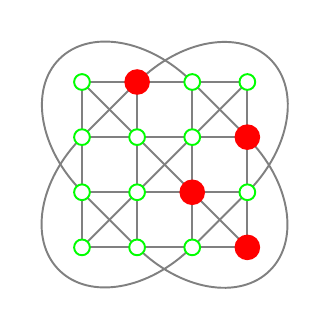
\begin{tikzpicture}  [scale=0.35]

\tikzstyle{every path}=[line width=0.7pt]

\newdimen\ms
\ms=0.1cm
\tikzstyle{s1}=[color=red,rectangle,inner sep=3.5]
\tikzstyle{c3}=[circle,inner sep={\ms/8},minimum size=4*\ms]
\tikzstyle{c2}=[circle,inner sep={\ms/8},minimum size=3*\ms]
\tikzstyle{c1}=[circle,inner sep={\ms/8},minimum size=2*\ms]
\tikzstyle{cs1}=[circle,inner sep={\ms/8},minimum size=1*\ms]

% Define positions of all observables

\coordinate (uuu) at ( 0,6);
\coordinate (uuv) at ( 2,6);
\coordinate (uvu) at ( 4,6);
\coordinate (uvv) at ( 6,6);
\coordinate (vuu) at ( 8,6);
\coordinate (vuv) at (10,6);
\coordinate (vvu) at (12,6);
\coordinate (vvv) at (14,6);

\coordinate (ucc) at ( 0,4);
\coordinate (vcc) at ( 2,4);
\coordinate (ucd) at ( 4,4);
\coordinate (vcd) at ( 6,4);
\coordinate (udc) at ( 8,4);
\coordinate (vdc) at (10,4);
\coordinate (udd) at (12,4);
\coordinate (vdd) at (14,4);

\coordinate (cuc) at ( 0,2);
\coordinate (cvc) at ( 2,2);
\coordinate (cud) at ( 4,2);
\coordinate (cvd) at ( 6,2);
\coordinate (duc) at ( 8,2);
\coordinate (dvc) at (10,2);
\coordinate (dud) at (12,2);
\coordinate (dvd) at (14,2);

\coordinate (ccu) at ( 0,0);
\coordinate (ccv) at ( 2,0);
\coordinate (cdu) at ( 4,0);
\coordinate (cdv) at ( 6,0);
\coordinate (dcu) at ( 8,0);
\coordinate (dcv) at (10,0);
\coordinate (ddu) at (12,0);
\coordinate (ddv) at (14,0);

% draw contexts

\draw [color=Gray] (ccu) -- (cdv);
\draw [color=Gray] (cuc) -- (cvd);
\draw [color=Gray] (ucc) -- (vcd);
\draw [color=Gray] (uuu) -- (uvv);

\draw [color=Gray] (uuu) -- (ccu);
\draw [color=Gray] (uuv) -- (ccv);
\draw [color=Gray] (uvu) -- (cdu);
\draw [color=Gray] (uvv) -- (cdv);

\draw [color=Gray] (uuu) -- (cdv);
\draw [color=Gray] (uvv) -- (ccu);

\draw [color=Gray] (uuv) -- (ucc);
\draw [color=Gray](cdu) -- (cvd);
\draw [rotate=225,color=Gray] (cvd) arc (90:270:4 and 2.82);
\draw[rotate=45,color=Gray] (ucc) arc (90:270:4 and 2.82);

\draw [color=Gray] (cuc) -- (ccv);
\draw [color=Gray] (uvu) -- (vcd);
\draw[rotate=315,color=Gray] (uvu) arc (90:270:4 and 2.82);
\draw[rotate=135,color=Gray] (ccv) arc (90:270:4 and 2.82);

%draw atoms

\draw (uuu) coordinate[c1,fill=white,draw=green];
\draw (uuv) coordinate[c2,fill=red,draw=red];
\draw (uvu) coordinate[c1,fill=white,draw=green];
\draw (uvv) coordinate[c1,fill=white,draw=green];


\draw (ucc) coordinate[c1,fill=white,draw=green];
\draw (vcc) coordinate[c1,fill=white,draw=green];
\draw (ucd) coordinate[c1,fill=white,draw=green];
\draw (vcd) coordinate[c2,fill=red,draw=red];

\draw (cuc) coordinate[c1,fill=white,draw=green];
\draw (cvc) coordinate[c1,fill=white,draw=green];
\draw (cud) coordinate[c2,fill=red,draw=red];
\draw (cvd) coordinate[c1,fill=white,draw=green];

\draw (ccu) coordinate[c1,fill=white,draw=green];
\draw (ccv) coordinate[c1,fill=white,draw=green];
\draw (cdu) coordinate[c1,fill=white,draw=green];
\draw (cdv) coordinate[c2,fill=red,draw=red];

\end{tikzpicture}
%
%
\\
%
%%%%%%%%%%% 5
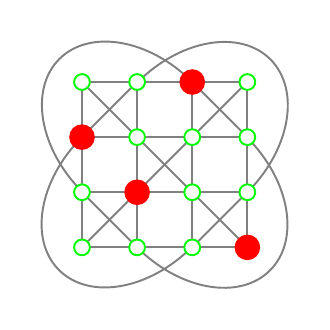
\begin{tikzpicture}  [scale=0.35]

\tikzstyle{every path}=[line width=0.7pt]

\newdimen\ms
\ms=0.1cm
\tikzstyle{s1}=[color=red,rectangle,inner sep=3.5]
\tikzstyle{c3}=[circle,inner sep={\ms/8},minimum size=4*\ms]
\tikzstyle{c2}=[circle,inner sep={\ms/8},minimum size=3*\ms]
\tikzstyle{c1}=[circle,inner sep={\ms/8},minimum size=2*\ms]
\tikzstyle{cs1}=[circle,inner sep={\ms/8},minimum size=1*\ms]

% Define positions of all observables

\coordinate (uuu) at ( 0,6);
\coordinate (uuv) at ( 2,6);
\coordinate (uvu) at ( 4,6);
\coordinate (uvv) at ( 6,6);
\coordinate (vuu) at ( 8,6);
\coordinate (vuv) at (10,6);
\coordinate (vvu) at (12,6);
\coordinate (vvv) at (14,6);

\coordinate (ucc) at ( 0,4);
\coordinate (vcc) at ( 2,4);
\coordinate (ucd) at ( 4,4);
\coordinate (vcd) at ( 6,4);
\coordinate (udc) at ( 8,4);
\coordinate (vdc) at (10,4);
\coordinate (udd) at (12,4);
\coordinate (vdd) at (14,4);

\coordinate (cuc) at ( 0,2);
\coordinate (cvc) at ( 2,2);
\coordinate (cud) at ( 4,2);
\coordinate (cvd) at ( 6,2);
\coordinate (duc) at ( 8,2);
\coordinate (dvc) at (10,2);
\coordinate (dud) at (12,2);
\coordinate (dvd) at (14,2);

\coordinate (ccu) at ( 0,0);
\coordinate (ccv) at ( 2,0);
\coordinate (cdu) at ( 4,0);
\coordinate (cdv) at ( 6,0);
\coordinate (dcu) at ( 8,0);
\coordinate (dcv) at (10,0);
\coordinate (ddu) at (12,0);
\coordinate (ddv) at (14,0);

% draw contexts

\draw [color=Gray] (ccu) -- (cdv);
\draw [color=Gray] (cuc) -- (cvd);
\draw [color=Gray] (ucc) -- (vcd);
\draw [color=Gray] (uuu) -- (uvv);

\draw [color=Gray] (uuu) -- (ccu);
\draw [color=Gray] (uuv) -- (ccv);
\draw [color=Gray] (uvu) -- (cdu);
\draw [color=Gray] (uvv) -- (cdv);

\draw [color=Gray] (uuu) -- (cdv);
\draw [color=Gray] (uvv) -- (ccu);

\draw [color=Gray] (uuv) -- (ucc);
\draw [color=Gray](cdu) -- (cvd);
\draw [rotate=225,color=Gray] (cvd) arc (90:270:4 and 2.82);
\draw[rotate=45,color=Gray] (ucc) arc (90:270:4 and 2.82);

\draw [color=Gray] (cuc) -- (ccv);
\draw [color=Gray] (uvu) -- (vcd);
\draw[rotate=315,color=Gray] (uvu) arc (90:270:4 and 2.82);
\draw[rotate=135,color=Gray] (ccv) arc (90:270:4 and 2.82);

%draw atoms

\draw (uuu) coordinate[c1,fill=white,draw=green];
\draw (uuv) coordinate[c1,fill=white,draw=green];
\draw (uvu) coordinate[c2,fill=red,draw=red];
\draw (uvv) coordinate[c1,fill=white,draw=green];


\draw (ucc) coordinate[c2,fill=red,draw=red];
\draw (vcc) coordinate[c1,fill=white,draw=green];
\draw (ucd) coordinate[c1,fill=white,draw=green];
\draw (vcd) coordinate[c1,fill=white,draw=green];

\draw (cuc) coordinate[c1,fill=white,draw=green];
\draw (cvc) coordinate[c2,fill=red,draw=red];
\draw (cud) coordinate[c1,fill=white,draw=green];
\draw (cvd) coordinate[c1,fill=white,draw=green];

\draw (ccu) coordinate[c1,fill=white,draw=green];
\draw (ccv) coordinate[c1,fill=white,draw=green];
\draw (cdu) coordinate[c1,fill=white,draw=green];
\draw (cdv) coordinate[c2,fill=red,draw=red];

\end{tikzpicture}
%
&
%
%%%%%%%%%%%%%%%%%%% 6
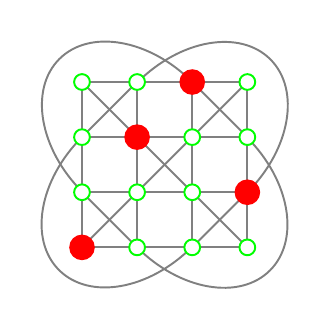
\begin{tikzpicture}  [scale=0.35]

\tikzstyle{every path}=[line width=0.7pt]

\newdimen\ms
\ms=0.1cm
\tikzstyle{s1}=[color=red,rectangle,inner sep=3.5]
\tikzstyle{c3}=[circle,inner sep={\ms/8},minimum size=4*\ms]
\tikzstyle{c2}=[circle,inner sep={\ms/8},minimum size=3*\ms]
\tikzstyle{c1}=[circle,inner sep={\ms/8},minimum size=2*\ms]
\tikzstyle{cs1}=[circle,inner sep={\ms/8},minimum size=1*\ms]

% Define positions of all observables

\coordinate (uuu) at ( 0,6);
\coordinate (uuv) at ( 2,6);
\coordinate (uvu) at ( 4,6);
\coordinate (uvv) at ( 6,6);
\coordinate (vuu) at ( 8,6);
\coordinate (vuv) at (10,6);
\coordinate (vvu) at (12,6);
\coordinate (vvv) at (14,6);

\coordinate (ucc) at ( 0,4);
\coordinate (vcc) at ( 2,4);
\coordinate (ucd) at ( 4,4);
\coordinate (vcd) at ( 6,4);
\coordinate (udc) at ( 8,4);
\coordinate (vdc) at (10,4);
\coordinate (udd) at (12,4);
\coordinate (vdd) at (14,4);

\coordinate (cuc) at ( 0,2);
\coordinate (cvc) at ( 2,2);
\coordinate (cud) at ( 4,2);
\coordinate (cvd) at ( 6,2);
\coordinate (duc) at ( 8,2);
\coordinate (dvc) at (10,2);
\coordinate (dud) at (12,2);
\coordinate (dvd) at (14,2);

\coordinate (ccu) at ( 0,0);
\coordinate (ccv) at ( 2,0);
\coordinate (cdu) at ( 4,0);
\coordinate (cdv) at ( 6,0);
\coordinate (dcu) at ( 8,0);
\coordinate (dcv) at (10,0);
\coordinate (ddu) at (12,0);
\coordinate (ddv) at (14,0);

% draw contexts

\draw [color=Gray] (ccu) -- (cdv);
\draw [color=Gray] (cuc) -- (cvd);
\draw [color=Gray] (ucc) -- (vcd);
\draw [color=Gray] (uuu) -- (uvv);

\draw [color=Gray] (uuu) -- (ccu);
\draw [color=Gray] (uuv) -- (ccv);
\draw [color=Gray] (uvu) -- (cdu);
\draw [color=Gray] (uvv) -- (cdv);

\draw [color=Gray] (uuu) -- (cdv);
\draw [color=Gray] (uvv) -- (ccu);

\draw [color=Gray] (uuv) -- (ucc);
\draw [color=Gray](cdu) -- (cvd);
\draw [rotate=225,color=Gray] (cvd) arc (90:270:4 and 2.82);
\draw[rotate=45,color=Gray] (ucc) arc (90:270:4 and 2.82);

\draw [color=Gray] (cuc) -- (ccv);
\draw [color=Gray] (uvu) -- (vcd);
\draw[rotate=315,color=Gray] (uvu) arc (90:270:4 and 2.82);
\draw[rotate=135,color=Gray] (ccv) arc (90:270:4 and 2.82);

%draw atoms

\draw (uuu) coordinate[c1,fill=white,draw=green];
\draw (uuv) coordinate[c1,fill=white,draw=green];
\draw (uvu) coordinate[c2,fill=red,draw=red];
\draw (uvv) coordinate[c1,fill=white,draw=green];


\draw (ucc) coordinate[c1,fill=white,draw=green];
\draw (vcc) coordinate[c2,fill=red,draw=red];
\draw (ucd) coordinate[c1,fill=white,draw=green];
\draw (vcd) coordinate[c1,fill=white,draw=green];

\draw (cuc) coordinate[c1,fill=white,draw=green];
\draw (cvc) coordinate[c1,fill=white,draw=green];
\draw (cud) coordinate[c1,fill=white,draw=green];
\draw (cvd) coordinate[c2,fill=red,draw=red];

\draw (ccu) coordinate[c2,fill=red,draw=red];
\draw (ccv) coordinate[c1,fill=white,draw=green];
\draw (cdu) coordinate[c1,fill=white,draw=green];
\draw (cdv) coordinate[c1,fill=white,draw=green];

\end{tikzpicture}
%
\\
%
%%%%%%%%%%% 7
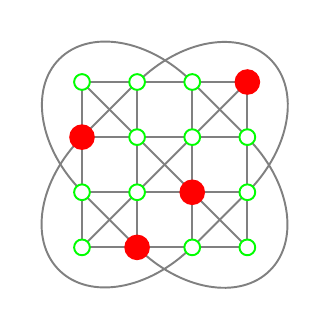
\begin{tikzpicture}  [scale=0.35]

\tikzstyle{every path}=[line width=0.7pt]

\newdimen\ms
\ms=0.1cm
\tikzstyle{s1}=[color=red,rectangle,inner sep=3.5]
\tikzstyle{c3}=[circle,inner sep={\ms/8},minimum size=4*\ms]
\tikzstyle{c2}=[circle,inner sep={\ms/8},minimum size=3*\ms]
\tikzstyle{c1}=[circle,inner sep={\ms/8},minimum size=2*\ms]
\tikzstyle{cs1}=[circle,inner sep={\ms/8},minimum size=1*\ms]

% Define positions of all observables

\coordinate (uuu) at ( 0,6);
\coordinate (uuv) at ( 2,6);
\coordinate (uvu) at ( 4,6);
\coordinate (uvv) at ( 6,6);
\coordinate (vuu) at ( 8,6);
\coordinate (vuv) at (10,6);
\coordinate (vvu) at (12,6);
\coordinate (vvv) at (14,6);

\coordinate (ucc) at ( 0,4);
\coordinate (vcc) at ( 2,4);
\coordinate (ucd) at ( 4,4);
\coordinate (vcd) at ( 6,4);
\coordinate (udc) at ( 8,4);
\coordinate (vdc) at (10,4);
\coordinate (udd) at (12,4);
\coordinate (vdd) at (14,4);

\coordinate (cuc) at ( 0,2);
\coordinate (cvc) at ( 2,2);
\coordinate (cud) at ( 4,2);
\coordinate (cvd) at ( 6,2);
\coordinate (duc) at ( 8,2);
\coordinate (dvc) at (10,2);
\coordinate (dud) at (12,2);
\coordinate (dvd) at (14,2);

\coordinate (ccu) at ( 0,0);
\coordinate (ccv) at ( 2,0);
\coordinate (cdu) at ( 4,0);
\coordinate (cdv) at ( 6,0);
\coordinate (dcu) at ( 8,0);
\coordinate (dcv) at (10,0);
\coordinate (ddu) at (12,0);
\coordinate (ddv) at (14,0);

% draw contexts

\draw [color=Gray] (ccu) -- (cdv);
\draw [color=Gray] (cuc) -- (cvd);
\draw [color=Gray] (ucc) -- (vcd);
\draw [color=Gray] (uuu) -- (uvv);

\draw [color=Gray] (uuu) -- (ccu);
\draw [color=Gray] (uuv) -- (ccv);
\draw [color=Gray] (uvu) -- (cdu);
\draw [color=Gray] (uvv) -- (cdv);

\draw [color=Gray] (uuu) -- (cdv);
\draw [color=Gray] (uvv) -- (ccu);

\draw [color=Gray] (uuv) -- (ucc);
\draw [color=Gray](cdu) -- (cvd);
\draw [rotate=225,color=Gray] (cvd) arc (90:270:4 and 2.82);
\draw[rotate=45,color=Gray] (ucc) arc (90:270:4 and 2.82);

\draw [color=Gray] (cuc) -- (ccv);
\draw [color=Gray] (uvu) -- (vcd);
\draw[rotate=315,color=Gray] (uvu) arc (90:270:4 and 2.82);
\draw[rotate=135,color=Gray] (ccv) arc (90:270:4 and 2.82);

%draw atoms

\draw (uuu) coordinate[c1,fill=white,draw=green];
\draw (uuv) coordinate[c1,fill=white,draw=green];
\draw (uvu) coordinate[c1,fill=white,draw=green];
\draw (uvv) coordinate[c2,fill=red,draw=red];


\draw (ucc) coordinate[c2,fill=red,draw=red];
\draw (vcc) coordinate[c1,fill=white,draw=green];
\draw (ucd) coordinate[c1,fill=white,draw=green];
\draw (vcd) coordinate[c1,fill=white,draw=green];

\draw (cuc) coordinate[c1,fill=white,draw=green];
\draw (cvc) coordinate[c1,fill=white,draw=green];
\draw (cud) coordinate[c2,fill=red,draw=red];
\draw (cvd) coordinate[c1,fill=white,draw=green];

\draw (ccu) coordinate[c1,fill=white,draw=green];
\draw (ccv) coordinate[c2,fill=red,draw=red];
\draw (cdu) coordinate[c1,fill=white,draw=green];
\draw (cdv) coordinate[c1,fill=white,draw=green];

\end{tikzpicture}
%
&
%
%%%%%%%%%%%%%%%%%%% 8
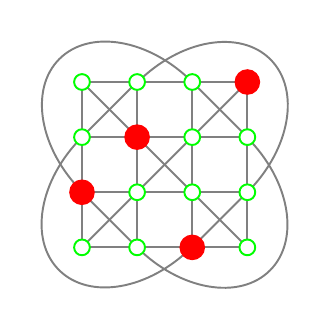
\begin{tikzpicture}  [scale=0.35]

\tikzstyle{every path}=[line width=0.7pt]

\newdimen\ms
\ms=0.1cm
\tikzstyle{s1}=[color=red,rectangle,inner sep=3.5]
\tikzstyle{c3}=[circle,inner sep={\ms/8},minimum size=4*\ms]
\tikzstyle{c2}=[circle,inner sep={\ms/8},minimum size=3*\ms]
\tikzstyle{c1}=[circle,inner sep={\ms/8},minimum size=2*\ms]
\tikzstyle{cs1}=[circle,inner sep={\ms/8},minimum size=1*\ms]

% Define positions of all observables

\coordinate (uuu) at ( 0,6);
\coordinate (uuv) at ( 2,6);
\coordinate (uvu) at ( 4,6);
\coordinate (uvv) at ( 6,6);
\coordinate (vuu) at ( 8,6);
\coordinate (vuv) at (10,6);
\coordinate (vvu) at (12,6);
\coordinate (vvv) at (14,6);

\coordinate (ucc) at ( 0,4);
\coordinate (vcc) at ( 2,4);
\coordinate (ucd) at ( 4,4);
\coordinate (vcd) at ( 6,4);
\coordinate (udc) at ( 8,4);
\coordinate (vdc) at (10,4);
\coordinate (udd) at (12,4);
\coordinate (vdd) at (14,4);

\coordinate (cuc) at ( 0,2);
\coordinate (cvc) at ( 2,2);
\coordinate (cud) at ( 4,2);
\coordinate (cvd) at ( 6,2);
\coordinate (duc) at ( 8,2);
\coordinate (dvc) at (10,2);
\coordinate (dud) at (12,2);
\coordinate (dvd) at (14,2);

\coordinate (ccu) at ( 0,0);
\coordinate (ccv) at ( 2,0);
\coordinate (cdu) at ( 4,0);
\coordinate (cdv) at ( 6,0);
\coordinate (dcu) at ( 8,0);
\coordinate (dcv) at (10,0);
\coordinate (ddu) at (12,0);
\coordinate (ddv) at (14,0);

% draw contexts

\draw [color=Gray] (ccu) -- (cdv);
\draw [color=Gray] (cuc) -- (cvd);
\draw [color=Gray] (ucc) -- (vcd);
\draw [color=Gray] (uuu) -- (uvv);

\draw [color=Gray] (uuu) -- (ccu);
\draw [color=Gray] (uuv) -- (ccv);
\draw [color=Gray] (uvu) -- (cdu);
\draw [color=Gray] (uvv) -- (cdv);

\draw [color=Gray] (uuu) -- (cdv);
\draw [color=Gray] (uvv) -- (ccu);

\draw [color=Gray] (uuv) -- (ucc);
\draw [color=Gray](cdu) -- (cvd);
\draw [rotate=225,color=Gray] (cvd) arc (90:270:4 and 2.82);
\draw[rotate=45,color=Gray] (ucc) arc (90:270:4 and 2.82);

\draw [color=Gray] (cuc) -- (ccv);
\draw [color=Gray] (uvu) -- (vcd);
\draw[rotate=315,color=Gray] (uvu) arc (90:270:4 and 2.82);
\draw[rotate=135,color=Gray] (ccv) arc (90:270:4 and 2.82);

%draw atoms

\draw (uuu) coordinate[c1,fill=white,draw=green];
\draw (uuv) coordinate[c1,fill=white,draw=green];
\draw (uvu) coordinate[c1,fill=white,draw=green];
\draw (uvv) coordinate[c2,fill=red,draw=red];


\draw (ucc) coordinate[c1,fill=white,draw=green];
\draw (vcc) coordinate[c2,fill=red,draw=red];
\draw (ucd) coordinate[c1,fill=white,draw=green];
\draw (vcd) coordinate[c1,fill=white,draw=green];

\draw (cuc) coordinate[c2,fill=red,draw=red];
\draw (cvc) coordinate[c1,fill=white,draw=green];
\draw (cud) coordinate[c1,fill=white,draw=green];
\draw (cvd) coordinate[c1,fill=white,draw=green];

\draw (ccu) coordinate[c1,fill=white,draw=green];
\draw (ccv) coordinate[c1,fill=white,draw=green];
\draw (cdu) coordinate[c2,fill=red,draw=red];
\draw (cdv) coordinate[c1,fill=white,draw=green];

\end{tikzpicture}
\end{tabular}
\end{center}
\caption{\label{2020-f-ghz-contextghz2vs}
Enumeration of the eight two-valued states of the ``tightened'' GHZ logic.
}
\end{figure}

From this partition logic, given by
\begin{equation}
\begin{aligned}
&\{ \{
\{1,2\},\{3,4\},\{5,6\},\{7,8\}
\},\\
&\{
\{5,7\},\{6,8\},\{1,3\},\{2,4\}
\},\\
&\{
\{3,8\},\{2,5\},\{4,7\},\{1,6\}
\},\\
&\{
\{4,6\},\{1,7\},\{2,8\},\{3,5\}
\},\\
&\{
\{1,2\},\{6,8\},\{4,7\},\{3,5\}
\},\\
&\{
\{7,8\},\{1,3\},\{2,5\},\{4,6\}
\},\\
&\{
\{5,6\},\{2,4\},\{3,8\},\{1,7\}
\},\\
&\{
\{3,4\},\{5,7\},\{1,6\},\{2,8\}
\}
\}
,
\end{aligned}
\label{2020-ghz-e-pl}
\end{equation}

one can immediately derive the classical probability distributions,
as well as a classical winning strategy for a GHZ-type game that is context-dependent but requires knowledge of the configuration or context involved.
All that is needed is the identification of the respective vertices in the original configuration and the partition logic
(any other variation within the horizontal contexts would also suffice);
e.g.,
$\{1,2\} \mapsto x_+x_+x_+$,
$\{3,4\} \mapsto x_+x_-x_-$, $\ldots$,
$\{2,8\} \mapsto y_+y_+x_-$.
The associated generalized urn model might match important aspects of the quantum mechanical predictions such as expectation values and distributions of order one, two, and three.

A typical experimental run would comprise a generalized urn ``loaded'' with (triples of identical) balls of eight types and four colors, associated with
the ward's potential choice of configurations or contexts.
Upon drawing such a ball triple the prisoners take their share of the triple---exactly one ball from the triple per prisoner---and, in accordance with the ward's choice,
read the pairs of numbers (from one to eight) in that respective color. Their choice must then be their position of the identified answer.
More explicitly, if they read ``$3,4$'' in the color associated with the first context,
the first prisoner writes or shouts ``$+$''1,
the second prisoner writes or shouts ``$-$''1,
the third prisoner writes or shouts ``$-$''1.
As has been mentioned earlier, any such value assignment is contextual in at least one observable $x$ or $y$; that is, for example, the first prisoner writes or shouts
different values for $x$ or $y$ for different contexts.


\section{Stranger-than-quantum GHZ games}

What if the prisoners would be given a ``magic filter'' or share capacity---say, a ``nonlocal'' (NL) or Popescu Rohrlich (PR) box~\cite{pop-rohr,svozil-krenn}---to go beyond quantum capacities of the GHZ game?
Suppose, for instance, that there are merely two prisoners involved, and four two-partite configurations or contexts
$xx$,
$xy$,
$yx$, and
$yy$; with the ward requesting as goal to achieve a negative product for $y\cdot y$
and else---that is, for $x\cdot x$, $x\cdot y$, and $y\cdot x$---positive products, as depicted in Figure~\ref{2020-f-ghz-contextconfstranger}.
Then again, by a parity argument such configurations cannot exist classically, because the observables $x$ and $y$ on either side contribute
to the overall product in pairs $x^2$ and $y^2$ which are always positive for real-valued $x$ and $y$;
but the ward requests a negative joint product
$\underbrace{(x\cdot x)}_{+1}\underbrace{(x\cdot y)}_{+1}\underbrace{(y\cdot x)}_{+1}\underbrace{(y\cdot y)}_{-1}=\left[ x^2 y^2\right]^2=(xy)^4=-1$
for real valued $x$ and $y$.

\begin{figure}[htb]%[H]
\begin{center}
\begin{tabular}{ c }
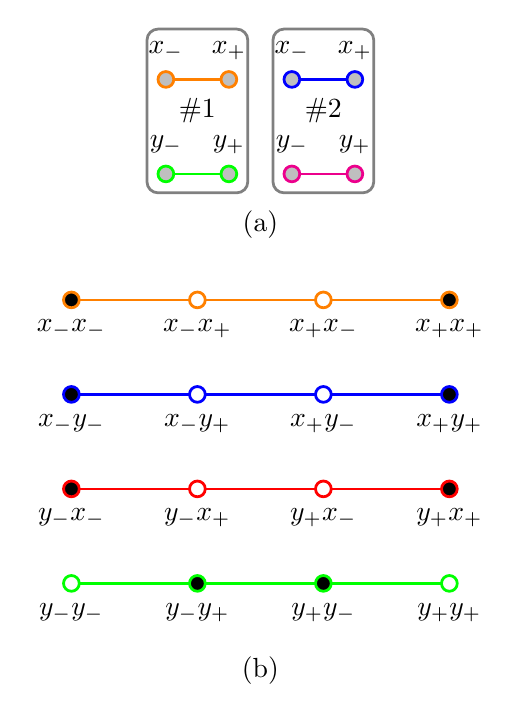
\begin{tikzpicture}  [scale=0.8]

\tikzstyle{every path}=[line width=1pt]

\newdimen\ms
\ms=0.1cm
\tikzstyle{s1}=[color=red,rectangle,inner sep=3.5]
\tikzstyle{c3}=[circle,inner sep={\ms/8},minimum size=4*\ms]
\tikzstyle{c2}=[circle,inner sep={\ms/8},minimum size=3*\ms]
\tikzstyle{c1}=[circle,inner sep={\ms/8},minimum size=2*\ms]
\tikzstyle{cs1}=[circle,inner sep={\ms/8},minimum size=1*\ms]

% Define positions of all observables


\coordinate (x11) at (1.5,8);
\coordinate (x12) at (2.5,8);
\coordinate (x21) at (3.5,8);
\coordinate (x22) at (4.5,8);

\coordinate (y11) at (1.5,6.5);
\coordinate (y12) at (2.5,6.5);
\coordinate (y21) at (3.5,6.5);
\coordinate (y22) at (4.5,6.5);

% draw contexts


\draw [color=orange] (x11) -- (x12);
\draw [color=blue] (x21) -- (x22);
\draw [color=green] (y11) -- (y12);
\draw [color=magenta] (y21) -- (y22);

% draw atoms

\draw (x11) coordinate[c1,fill=Gray!50, draw=orange,label=above:$x_-$];
\draw (x12) coordinate[c1,fill=Gray!50, draw=orange,label=above:$x_+$];
\draw (x21) coordinate[c1,fill=Gray!50, draw=blue,label=above:$x_-$];
\draw (x22) coordinate[c1,fill=Gray!50, draw=blue,label=above:$x_+$];

\draw (y11) coordinate[c1,fill=Gray!50, draw=green,label=above:$y_-$];
\draw (y12) coordinate[c1,fill=Gray!50, draw=green,label=above:$y_+$];
\draw (y21) coordinate[c1,fill=Gray!50, draw=magenta,label=above:$y_-$];
\draw (y22) coordinate[c1,fill=Gray!50, draw=magenta,label=above:$y_+$];

\draw[Gray,rounded corners] (1.2, 6.2) rectangle (2.8, 8.8) node[black,pos=.5] {{\#}1};
\draw[Gray,rounded corners] (3.2, 6.2) rectangle (4.8, 8.8) node[black,pos=.5] {{\#}2};

\coordinate (a) at (3,5.3);
\draw (a) coordinate[label=above:(a)];


% Define positions of all observables

\coordinate (ccu) at (0,4.5);
\coordinate (cdu) at (2,4.5);
\coordinate (dcu) at (4,4.5);
\coordinate (ddu) at (6,4.5);

\coordinate (cuc) at (0,3);
\coordinate (cud) at (2,3);
\coordinate (duc) at (4,3);
\coordinate (dud) at (6,3);

\coordinate (ucc) at (0,1.5);
\coordinate (ucd) at (2,1.5);
\coordinate (udc) at (4,1.5);
\coordinate (udd) at (6,1.5);

\coordinate (uuu) at (0,0);
\coordinate (uvu) at (2,0);
\coordinate (vuu) at (4,0);
\coordinate (vvu) at (6,0);

% draw contexts

\draw [color=orange] (ccu) -- (ddu);
\draw [color=blue] (cuc) -- (dud);
\draw [color=red] (ucc) -- (udd);
\draw [color=green] (uuu) -- (vvu);



% draw atoms

\draw (ccu) coordinate[c1,fill=black, draw=orange,label=below:$x_-  x_-$];
\draw (cdu) coordinate[c1,fill=white, draw=orange,label=below:$x_-  x_+$];
\draw (dcu) coordinate[c1,fill=white, draw=orange,label=below:$x_+  x_-$];
\draw (ddu) coordinate[c1,fill=black, draw=orange,label=below:$x_+  x_+$];

\draw (cuc) coordinate[c1,fill=black, draw=blue,label=below:$x_-  y_-$];
\draw (cud) coordinate[c1,fill=white, draw=blue,label=below:$x_-  y_+$];
\draw (duc) coordinate[c1,fill=white, draw=blue,label=below:$x_+  y_-$];
\draw (dud) coordinate[c1,fill=black, draw=blue,label=below:$x_+  y_+$];

\draw (ucc) coordinate[c1,fill=black, draw=red,label=below:$y_-  x_-$];
\draw (ucd) coordinate[c1,fill=white, draw=red,label=below:$y_-  x_+$];
\draw (udc) coordinate[c1,fill=white, draw=red,label=below:$y_+  x_-$];
\draw (udd) coordinate[c1,fill=black, draw=red,label=below:$y_+  x_+$];

\draw (uuu) coordinate[c1,fill=white, draw=green,label=below:$y_-  y_-$];
\draw (uvu) coordinate[c1,fill=black, draw=green,label=below:$y_-  y_+$];
\draw (vuu) coordinate[c1,fill=black, draw=green,label=below:$y_+  y_-$];
\draw (vvu) coordinate[c1,fill=white, draw=green,label=below:$y_+  y_+$];

\coordinate (b) at (3,-1);
\draw (b) coordinate[label=below:(b)];

\end{tikzpicture}
\end{tabular}
\end{center}
\caption{\label{2020-f-ghz-contextconfstranger}
Hypergraphs representing
(a) the four disconnected classical single-particle contexts---two contexts per particle---representing the observables of the first and second particle, respectively;
(b) the four separated, nonintertwined two-partite contexts, with four atoms each, that are the Cartesian products of these single-particle contexts.
Filled circles indicate states which are involved in a stranger-than-GHZ game
requesting positivity for all products  $xx=xy=yx=+1$ and  negativityfor $yy=-1$.
}
\end{figure}

For a proof that this configuration has no quantum realization
we take (overline indicates complex conjugation)
$\vert x_+ \rangle =\begin{pmatrix} x_{+,1} , x_{+,2} \end{pmatrix}^\intercal$,
$\vert x_- \rangle =\begin{pmatrix} \overline{x}_{+,2} , -\overline{x}_{+,1}  \end{pmatrix}^\intercal$,
$\vert y_+ \rangle =\begin{pmatrix} y_{+,1} , y_{+,2} \end{pmatrix}^\intercal$,
$\vert y_- \rangle =\begin{pmatrix} \overline{y}_{+,2} , -\overline{y}_{+,1}  \end{pmatrix}^\intercal$,
and $\vert \psi \rangle = \begin{pmatrix} \psi_1,\psi_2,\psi_3,\psi_4 \end{pmatrix}^\intercal$.
The stranger-than-GHZ game rules require that
$
\langle  \psi  \vert  x_+ x_+ \rangle =
\langle  \psi  \vert  x_- x_- \rangle =
\langle  \psi  \vert  x_+ y_+ \rangle =
\langle  \psi  \vert  x_- y_- \rangle =
\langle  \psi  \vert  y_+ x_+ \rangle =
\langle  \psi  \vert  y_- x_- \rangle =
\langle  \psi  \vert  y_+ y_- \rangle =
\langle  \psi  \vert  y_- y_+ \rangle = 0$.
Without loss of generality we may fix $x_{+,2}=0$, and, because of symmetry, $y_{+,1} = y_{+,2} = 1/\sqrt{2}$,
which admits only the trivial solution  $\vert \psi \rangle = \begin{pmatrix}0,0,0,0 \end{pmatrix}^\intercal$.

The situation is ``contextual'' as any realization involves context-dependence of either the $x$ or the $y$-observables.
Suppose the prisoners have at their disposal a NL PR box of the following capacity:
if $i_1$ and $i_2$ stand for the inputs of the box, and $o_1$ and $o_2$ for its outputs, then
$
i_1 i_2 = o_1 \oplus o_2 = o_1 + o_2 \text{ mod }2$.
Now if both prisoners ``translate their in- and outputs'' as follows:
they input 0 on an "x" input, and 1 on a "y" input,
as well as identify  ``$+$''1 with output 0 and ``$-$''1 with output 1, respectively.
Then, if the in- and outputs are ordered by prisoner,
\begin{equation}
\begin{aligned}
x,x & \mapsto   0 \cdot 0 = 0 \stackrel{\text{NL PR}}{\xrightarrow{\hspace*{6mm}}} \{0 \oplus 0 \text{  or  } 1 \oplus 1\} \mapsto   \{++,--\}     ,\\
x,y & \mapsto   0 \cdot 1 = 0 \stackrel{\text{NL PR}}{\xrightarrow{\hspace*{6mm}}} \{0 \oplus 0 \text{  or  } 1 \oplus 1\} \mapsto   \{++,--\}     ,\\
y,x & \mapsto   1 \cdot 0 = 0 \stackrel{\text{NL PR}}{\xrightarrow{\hspace*{6mm}}} \{0 \oplus 0 \text{  or  } 1 \oplus 1\} \mapsto   \{++,--\}     ,\\
y,y & \mapsto   1 \cdot 1 = 1 \stackrel{\text{NL PR}}{\xrightarrow{\hspace*{6mm}}} \{0 \oplus 1 \text{  or  } 1 \oplus 0\} \mapsto   \{+-,-+\}     .
\end{aligned}
\end{equation}
This perfect winning strategy can be further specified~\cite{PhysRevA.71.022101} by
the joint outcome probabilities
$P \left( o_1,o_2 \vert i_1,i_2 \right) = \frac{1}{2}$ for $i_1 i_2 = o_1 \oplus o_2 = o_1 + o_2$ and vanishing otherwise.
For a game requiring
$\underbrace{(x\cdot x)}_{-1}\underbrace{(x\cdot y)}_{-1}\underbrace{(y\cdot x)}_{-1}\underbrace{(y\cdot y)}_{+1}=-1$
one of the prisoners would need to switch the output behaviour $+ \longleftrightarrow -$.
Indeed the NL PR box appears to be a direct realization of a winning strategy  for the stranger-than-GHZ game.

\section{Some afterthoughts}



From a quantum logical point of view the GHZ argument differs
from the KS argument in its fairly simplistic geometric and algebraic structure involving only four isolated contexts
instead of a collection of intertwining contexts.
Indeed, it might be amazing how much quantum-versus classical discord can be gained from such configuration.
Unlike the KS configuration which is based on the total absence of two-valued states interpretable as classical truth assignments,
the observables involved in GHZ allow a plethora (namely $8^4$) of such states which are separating~\cite[Theorem~0]{kochen1}.

The strength of the GHZ argument lies not in the scarcity of two-valued states
but in the proper---that is, suitable for, and adapted to, the particular task---reduction or ``filtering'' the respective eigenstates, which serve as elements of the contexts,
by the state preparation or selection.
Thereby some nonclassical features can be claimed relative to the assumptions.

This is not dissimilar to ``Hardy-type'' configurations in which a particular particle or a multi-partite state is prepared and---by the classical interpretation
of a configuration of observables forming intertwining contexts---``viewed'' by another observable or proposition~\cite{svozil-2020-hardy}.
In particular, if such a configuration with a true-implies-true set of two-valued states (TITS)~\cite{2018-minimalYIYS}
has ``orthogonal arperture'' (that is, orthogonality between the prepared and the measured state)
the classical prediction is in direct contradiction with the quantum expectation of nonoccurence because of orthogonality.
This has already been realized by KS as subgraphs of their $\Gamma_2$---they render the orthogonal aperture by a serial composition of TITS (their $\Gamma_1$)
with less than $\frac{\pi}{2}$ between the states prepared and measured~\cite{kochen1}.

Another difference to KS and Hardy-type arguments comes from the fact that its predictions are obtained by multiplying nonvanishing values in $\{-1,+1\}$
of the experimental outcomes instead of working with dispersionless $\{0,1\}$ two-valued states which include the value $0$.
Taking nonvanishing values $\{-1,+1\}$ preserves much more information and structure about the joint observables than in the $\{0,1\}$ case.
Because while for a single two-state particle
any $\{-1,+1\}$-observable $\textsf{\textbf{A}}$ can be considered an affine transformation
of the two-valued state $s \in \{0,1\}$ by $\textsf{\textbf{A}} = 2 s - 1$
(that corresponds to the negative of a quantum Householder transformation
$\textsf{\textbf{U}}
=
\mathbb{1}- 2  \vert {\bf x} \rangle \langle  {\bf x}  \vert$ for a unit vector $\vert {\bf x} \rangle$),
there is no loss of information due to this linear transformation,
this is in general not true in the multi-partite situation; in particular, with three particles involved:
whereas in the  $\{0,1\}$ case all products vanish except in the case for which the outcome is 1 on all three particles simultaneously,
the products of possible  $\{-1,+1\}$ cases show a much more balanced partitioning:
parity dictates that there is equidistribution (50:50) of joint negative and positive outcomes.
Formally, in terms of entropy, the  $\{0,1\}$  case results in
$H_{\{0,1\}^3} = -\frac{1}{8} \log_2 \frac{1}{8} -  \frac{7}{8} \log_2 \frac{7}{8}   \approx 0.54$
as compared to the  $\{-1,+1\}$ case which yields
$H_{\{-1,+1\}^3} = -\frac{1}{2} \log_2 \frac{1}{2} -  \frac{1}{2} \log_2 \frac{1}{2}  =1$.
Therefore, the latter three-partite $\{-1,+1\}$ outcome case results in an average rate of ``information'' inherent in the variable's potential outcomes
which is almost twice as high as in the  $\{0,1\}$  case.
%So, as can be expected, by translating admissibility criteria (such as exclusivity and completeness) from the two-valued case
%into the operator eigenvalue case, it is possible~\cite{cabello-96,Xu-Chen-Guehnw-2020} to rephrase a KS argument
%in terms of an operator based argument.
One straightforward way of enhancing the ``contrast'' or violation between classical and quantum predictions would be to
consider Operators with eigenvalues $\{-\lambda,+\lambda\}$ larger that in the ones chosen for the GHZ argument; that is, $1\ll \lambda $.
The respective observables correspond to operators whose spectral sum includes the same orthogonal projection operators as the operators~(\ref{2020-ghz-sigmas-contextop})
involved in the GHZ case. These orthogonal projection operators are
formed by the dyadic products of the vectors~(\ref{2020-ghz-evsisjsk}).



This review is the continuation of an ongoing effort~\cite{svozil-2017-b,svozil-2020-hardy}
to transcribe and (de)construct well-known arguments from the foundations of quantum mechanics into a logico-algebraic context.
The operators of the GHZ argument had to be delineated in terms of their spectral form, revealing the propositional structure in terms of the
orthogonal projection operators. Since the argument is state dependent, the valuations of these elementary propositional observables
had to be taken for the particular state involved.
My aim has been to obtain insights into the structural properties of the arguments,
as well as transparent and effective presentations and derivations
of the predictions and probabilities supported by the respective configurations.

Following the aforementioned effort, the conceptual take-home message of the paper is this: the GHZ argument can be readily ``embedded'' into,
or translated and presented, in terms of the quantum logical framework of Birkhoff and von Neumann~\cite{birkhoff-36}
as well as partial algebras~\cite{kochen2,kochen3} and orthomodular structures~\cite{kalmbach-83,pulmannova-91}.
From a formal point of view, this allows its uniform presentation and comparison to ``competing'' and related arguments,
such as Hardy-type or KS arguments.
From an empirical point of view, the operator-based approach facilitates operational extensions and generalizations of the original argument.





\begin{acknowledgments}
This research was funded in whole, or in part, by the Austrian Science Fund (FWF), Project No. I 4579-N. For the purpose of open access, the author has applied a CC BY public copyright licence to any Author Accepted Manuscript version arising from this submission.
%The author acknowledges the support by the Austrian Science Fund (FWF): project I 4579-N and the Czech Science Foundation (GA\v CR): project 20-09869L.

I kindly acknowledge discussions with and corrections by Peter Morgan, as well as a hint by Anne Broadbent with regards to realizations of stranger-than-quantum GHZ games by NL PR boxes.
%I kindly acknowledge enlightening discussions with Adan Cabello, Hans Havlicek, Norman Megill, Mladen Pavi{\v{c}}i{\'{c}}, Jos\'{e} R. Portillo, and Mohammad Hadi Shekarriz.
%I am grateful to Josef Tkadlec for providing a {\em Pascal} program which computes and analyses the set of two-valued states of collections of contexts.
%I am also grateful to  Norman D. Megill and Mladen Pavi{\v{c}}i{\'{c}} for providing a {\em C++} program which computes the faithful orthogonal representations of hypergraphs written in MMP format, given possible vector components.
All misconceptions and errors are mine.

The author declares no conflict of interest.
\end{acknowledgments}



% MDPI \funding{The author acknowledges the support by the Austrian Science Fund (FWF): project I 4579-N and the Czech Science Foundation (GA\v CR): project 20-09869L.}

%%%%%%%%%%%%%%%%%%%%%%%%%%%%%%%%%%%%%%%
% MDPI \acknowledgments{I kindly acknowledge enlightening discussions with Adan Cabello, Jos\'{e} R. Portillo, and Mohammad Hadi Shekarriz.
% MDPI I am grateful to Josef Tkadlec for providing a {\em Pascal} program
% MDPI which computes and analyses the set of two-valued states of collections of contexts.
% MDPI All misconceptions and errors are mine.
% MDPI The author declares no conflict of interest.
% MDPI }

%%%%%%%%%%%%%%%%%%%%%%%%%%%%%%%%%%%%%%%
% MDPI \conflictsofinterest{The author declares no conflict of interest.}


%%%%%%%%%%%%%%%%%%%%%%%%%%%%%%%%%%%%%%%
% MDPI \reftitle{References}

% Please provide either the correct journal abbreviation (e.g. according to the “List of Title Word Abbreviations” http://www.issn.org/services/online-services/access-to-the-ltwa/) or the full name of the journal.
% Citations and References in Supplementary files are permitted provided that they also appear in the reference list here.

%=====================================
% References, variant A: external bibliography
%=====================================
%\externalbibliography{yes}

%\bibliography{svozil}


%merlin.mbs apsrev4-1.bst 2010-07-25 4.21a (PWD, AO, DPC) hacked
%Control: key (0)
%Control: author (0) dotless jnrlst
%Control: editor formatted (1) identically to author
%Control: production of article title (0) allowed
%Control: page (1) range
%Control: year (0) verbatim
%Control: production of eprint (0) enabled
\begin{thebibliography}{55}%
\makeatletter
\providecommand \@ifxundefined [1]{%
 \@ifx{#1\undefined}
}%
\providecommand \@ifnum [1]{%
 \ifnum #1\expandafter \@firstoftwo
 \else \expandafter \@secondoftwo
 \fi
}%
\providecommand \@ifx [1]{%
 \ifx #1\expandafter \@firstoftwo
 \else \expandafter \@secondoftwo
 \fi
}%
\providecommand \natexlab [1]{#1}%
\providecommand \enquote  [1]{``#1''}%
\providecommand \bibnamefont  [1]{#1}%
\providecommand \bibfnamefont [1]{#1}%
\providecommand \citenamefont [1]{#1}%
\providecommand \href@noop [0]{\@secondoftwo}%
\providecommand \href [0]{\begingroup \@sanitize@url \@href}%
\providecommand \@href[1]{\@@startlink{#1}\@@href}%
\providecommand \@@href[1]{\endgroup#1\@@endlink}%
\providecommand \@sanitize@url [0]{\catcode `\\12\catcode `\$12\catcode
  `\&12\catcode `\#12\catcode `\^12\catcode `\_12\catcode `\%12\relax}%
\providecommand \@@startlink[1]{}%
\providecommand \@@endlink[0]{}%
\providecommand \url  [0]{\begingroup\@sanitize@url \@url }%
\providecommand \@url [1]{\endgroup\@href {#1}{\urlprefix }}%
\providecommand \urlprefix  [0]{URL }%
\providecommand \Eprint [0]{\href }%
\providecommand \doibase [0]{http://dx.doi.org/}%
\providecommand \selectlanguage [0]{\@gobble}%
\providecommand \bibinfo  [0]{\@secondoftwo}%
\providecommand \bibfield  [0]{\@secondoftwo}%
\providecommand \translation [1]{[#1]}%
\providecommand \BibitemOpen [0]{}%
\providecommand \bibitemStop [0]{}%
\providecommand \bibitemNoStop [0]{.\EOS\space}%
\providecommand \EOS [0]{\spacefactor3000\relax}%
\providecommand \BibitemShut  [1]{\csname bibitem#1\endcsname}%
\let\auto@bib@innerbib\@empty
%</preamble>
\bibitem [{\citenamefont {Greenberger}\ \emph {et~al.}(1989)\citenamefont
  {Greenberger}, \citenamefont {Horne},\ and\ \citenamefont {Zeilinger}}]{ghz}%
  \BibitemOpen
  \bibfield  {author} {\bibinfo {author} {\bibfnamefont {Daniel~M.}\
  \bibnamefont {Greenberger}}, \bibinfo {author} {\bibfnamefont {Mike~A.}\
  \bibnamefont {Horne}}, \ and\ \bibinfo {author} {\bibfnamefont {Anton}\
  \bibnamefont {Zeilinger}},\ }\bibfield  {title} {\enquote {\bibinfo {title}
  {Going beyond {B}ell's theorem},}\ }in\ \href {\doibase
  10.1007/978-94-017-0849-4\_10} {\emph {\bibinfo {booktitle} {Bell's Theorem,
  Quantum Theory, and Conceptions of the {U}niverse}}},\ \bibinfo {series}
  {Fundamental Theories of Physics}, Vol.~\bibinfo {volume} {37},\ \bibinfo
  {editor} {edited by\ \bibinfo {editor} {\bibfnamefont {Menas}\ \bibnamefont
  {Kafatos}}}\ (\bibinfo  {publisher} {Kluwer Academic Publishers, Springer
  Netherlands},\ \bibinfo {address} {Dordrecht},\ \bibinfo {year} {1989})\ pp.\
  \bibinfo {pages} {69--72},\ \Eprint
  {http://arxiv.org/abs/http://arxiv.org/abs/0712.0921}
  {http://arxiv.org/abs/0712.0921} \BibitemShut {NoStop}%
\bibitem [{\citenamefont {Mermin}(2007)}]{mermin-07}%
  \BibitemOpen
  \bibfield  {author} {\bibinfo {author} {\bibfnamefont {David~N.}\
  \bibnamefont {Mermin}},\ }\href {\doibase 10.1017/CBO9780511813870} {\emph
  {\bibinfo {title} {Quantum Computer Science}}}\ (\bibinfo  {publisher}
  {Cambridge University Press},\ \bibinfo {address} {Cambridge},\ \bibinfo
  {year} {2007})\BibitemShut {NoStop}%
\bibitem [{\citenamefont {Schr{\"{o}}dinger}(1935)}]{schrodinger-gwsidqm2}%
  \BibitemOpen
  \bibfield  {author} {\bibinfo {author} {\bibfnamefont {Erwin}\ \bibnamefont
  {Schr{\"{o}}dinger}},\ }\bibfield  {title} {\enquote {\bibinfo {title} {{D}ie
  gegenw\"artige {S}ituation in der {Q}uantenmechanik},}\ }\href {\doibase
  10.1007/BF01491914} {\bibfield  {journal} {\bibinfo  {journal}
  {Naturwissenschaften}\ }\textbf {\bibinfo {volume} {23}},\ \bibinfo {pages}
  {823--828} (\bibinfo {year} {1935})}\BibitemShut {NoStop}%
\bibitem [{\citenamefont {Zeilinger}(1999)}]{zeil-99}%
  \BibitemOpen
  \bibfield  {author} {\bibinfo {author} {\bibfnamefont {Anton}\ \bibnamefont
  {Zeilinger}},\ }\bibfield  {title} {\enquote {\bibinfo {title} {A
  foundational principle for quantum mechanics},}\ }\href {\doibase
  10.1023/A:1018820410908} {\bibfield  {journal} {\bibinfo  {journal}
  {Foundations of Physics}\ }\textbf {\bibinfo {volume} {29}},\ \bibinfo
  {pages} {631--643} (\bibinfo {year} {1999})}\BibitemShut {NoStop}%
\bibitem [{\citenamefont {Svozil}(2018{\natexlab{a}})}]{svozil-2016-sampling}%
  \BibitemOpen
  \bibfield  {author} {\bibinfo {author} {\bibfnamefont {Karl}\ \bibnamefont
  {Svozil}},\ }\bibfield  {title} {\enquote {\bibinfo {title} {A note on the
  statistical sampling aspect of delayed choice entanglement swapping},}\ }in\
  \href {\doibase 10.1142/9789813276895\_0001} {\emph {\bibinfo {booktitle}
  {Probing the Meaning of Quantum Mechanics}}}\ (\bibinfo  {publisher} {World
  Scientific},\ \bibinfo {address} {Singapore},\ \bibinfo {year} {2018})\ pp.\
  \bibinfo {pages} {1--9},\ \Eprint {http://arxiv.org/abs/arXiv:1608.04984}
  {arXiv:1608.04984} \BibitemShut {NoStop}%
\bibitem [{\citenamefont {Kochen}\ and\ \citenamefont
  {Specker}(1967)}]{kochen1}%
  \BibitemOpen
  \bibfield  {author} {\bibinfo {author} {\bibfnamefont {Simon}\ \bibnamefont
  {Kochen}}\ and\ \bibinfo {author} {\bibfnamefont {Ernst~P.}\ \bibnamefont
  {Specker}},\ }\bibfield  {title} {\enquote {\bibinfo {title} {The problem of
  hidden variables in quantum mechanics},}\ }\href {\doibase
  10.1512/iumj.1968.17.17004} {\bibfield  {journal} {\bibinfo  {journal}
  {Journal of Mathematics and Mechanics (now Indiana University Mathematics
  Journal)}\ }\textbf {\bibinfo {volume} {17}},\ \bibinfo {pages} {59--87}
  (\bibinfo {year} {1967})}\BibitemShut {NoStop}%
\bibitem [{\citenamefont {Xu}\ \emph {et~al.}(2020)\citenamefont {Xu},
  \citenamefont {Chen},\ and\ \citenamefont {G\"uhne}}]{Xu-Chen-Guehnw-2020}%
  \BibitemOpen
  \bibfield  {author} {\bibinfo {author} {\bibfnamefont {Zhen-Peng}\
  \bibnamefont {Xu}}, \bibinfo {author} {\bibfnamefont {Jing-Ling}\
  \bibnamefont {Chen}}, \ and\ \bibinfo {author} {\bibfnamefont {Otfried}\
  \bibnamefont {G\"uhne}},\ }\href {\doibase 10.1103/PhysRevLett.124.230401}
  {\enquote {\bibinfo {title} {Proof of the {P}eres conjecture for
  contextuality},}\ } (\bibinfo {year} {2020}),\ \Eprint
  {http://arxiv.org/abs/arXiv:2001.07656} {arXiv:2001.07656} \BibitemShut
  {NoStop}%
\bibitem [{\citenamefont {Cabello}(2021)}]{cabello2020converting}%
  \BibitemOpen
  \bibfield  {author} {\bibinfo {author} {\bibfnamefont {Ad\'an}\ \bibnamefont
  {Cabello}},\ }\bibfield  {title} {\enquote {\bibinfo {title} {Converting
  contextuality into nonlocality},}\ }\href {\doibase
  10.1103/PhysRevLett.127.070401} {\bibfield  {journal} {\bibinfo  {journal}
  {Physical Review Letters}\ }\textbf {\bibinfo {volume} {127}},\ \bibinfo
  {pages} {070401} (\bibinfo {year} {2021})},\ \Eprint
  {http://arxiv.org/abs/arXiv:2011.13790} {arXiv:2011.13790} \BibitemShut
  {NoStop}%
\bibitem [{\citenamefont {Hardy}(1993)}]{Hardy-93}%
  \BibitemOpen
  \bibfield  {author} {\bibinfo {author} {\bibfnamefont {Lucien}\ \bibnamefont
  {Hardy}},\ }\bibfield  {title} {\enquote {\bibinfo {title} {Nonlocality for
  two particles without inequalities for almost all entangled states},}\ }\href
  {\doibase 10.1103/PhysRevLett.71.1665} {\bibfield  {journal} {\bibinfo
  {journal} {Physical Review Letters}\ }\textbf {\bibinfo {volume} {71}},\
  \bibinfo {pages} {1665--1668} (\bibinfo {year} {1993})}\BibitemShut {NoStop}%
\bibitem [{\citenamefont {Svozil}(2021)}]{svozil-2020-hardy}%
  \BibitemOpen
  \bibfield  {author} {\bibinfo {author} {\bibfnamefont {Karl}\ \bibnamefont
  {Svozil}},\ }\bibfield  {title} {\enquote {\bibinfo {title} {Extensions of
  {H}ardy-type true-implies-false gadgets to classically obtain
  indistinguishability},}\ }\href {\doibase 10.1103/PhysRevA.103.022204}
  {\bibfield  {journal} {\bibinfo  {journal} {Physical Review A}\ }\textbf
  {\bibinfo {volume} {103}},\ \bibinfo {pages} {022204} (\bibinfo {year}
  {2021})},\ \Eprint {http://arxiv.org/abs/arXiv:2006.11396} {arXiv:2006.11396}
  \BibitemShut {NoStop}%
\bibitem [{\citenamefont {Svozil}(2009)}]{svozil-2006-omni}%
  \BibitemOpen
  \bibfield  {author} {\bibinfo {author} {\bibfnamefont {Karl}\ \bibnamefont
  {Svozil}},\ }\bibfield  {title} {\enquote {\bibinfo {title} {Quantum
  scholasticism: On quantum contexts, counterfactuals, and the absurdities of
  quantum omniscience},}\ }\href {\doibase 10.1016/j.ins.2008.06.012}
  {\bibfield  {journal} {\bibinfo  {journal} {Information Sciences}\ }\textbf
  {\bibinfo {volume} {179}},\ \bibinfo {pages} {535--541} (\bibinfo {year}
  {2009})}\BibitemShut {NoStop}%
\bibitem [{\citenamefont {Cabello}\ \emph {et~al.}(2018)\citenamefont
  {Cabello}, \citenamefont {Portillo}, \citenamefont {Sol\'{i}s},\ and\
  \citenamefont {Svozil}}]{2018-minimalYIYS}%
  \BibitemOpen
  \bibfield  {author} {\bibinfo {author} {\bibfnamefont {Ad\'an}\ \bibnamefont
  {Cabello}}, \bibinfo {author} {\bibfnamefont {Jos\'{e}~R.}\ \bibnamefont
  {Portillo}}, \bibinfo {author} {\bibfnamefont {Alberto}\ \bibnamefont
  {Sol\'{i}s}}, \ and\ \bibinfo {author} {\bibfnamefont {Karl}\ \bibnamefont
  {Svozil}},\ }\bibfield  {title} {\enquote {\bibinfo {title} {Minimal
  true-implies-false and true-implies-true sets of propositions in
  noncontextual hidden-variable theories},}\ }\href {\doibase
  10.1103/PhysRevA.98.012106} {\bibfield  {journal} {\bibinfo  {journal}
  {Physical Review A}\ }\textbf {\bibinfo {volume} {98}},\ \bibinfo {pages}
  {012106} (\bibinfo {year} {2018})},\ \Eprint
  {http://arxiv.org/abs/arXiv:1805.00796} {arXiv:1805.00796} \BibitemShut
  {NoStop}%
\bibitem [{\citenamefont {Holweck}\ and\ \citenamefont
  {Saniga}(2017)}]{Holweck2017}%
  \BibitemOpen
  \bibfield  {author} {\bibinfo {author} {\bibfnamefont {Fr\'ed\'eric}\
  \bibnamefont {Holweck}}\ and\ \bibinfo {author} {\bibfnamefont {Metod}\
  \bibnamefont {Saniga}},\ }\bibfield  {title} {\enquote {\bibinfo {title}
  {Contextuality with a small number of observables},}\ }\href {\doibase
  10.1142/s0219749917500265} {\bibfield  {journal} {\bibinfo  {journal}
  {International Journal of Quantum Information}\ }\textbf {\bibinfo {volume}
  {15}},\ \bibinfo {pages} {1750026} (\bibinfo {year} {2017})},\ \Eprint
  {http://arxiv.org/abs/arXiv:1607.07567} {arXiv:1607.07567} \BibitemShut
  {NoStop}%
\bibitem [{\citenamefont {Halmos}(1958)}]{halmos-vs}%
  \BibitemOpen
  \bibfield  {author} {\bibinfo {author} {\bibfnamefont {Paul~Richard}\
  \bibnamefont {Halmos}},\ }\href {\doibase 10.1007/978-1-4612-6387-6} {\emph
  {\bibinfo {title} {Finite-Dimensional Vector Spaces}}},\ Undergraduate Texts
  in Mathematics\ (\bibinfo  {publisher} {Springer},\ \bibinfo {address} {New
  York},\ \bibinfo {year} {1958})\BibitemShut {NoStop}%
\bibitem [{\citenamefont {Bacon}(2006)}]{bacon-ghzgames-2006}%
  \BibitemOpen
  \bibfield  {author} {\bibinfo {author} {\bibfnamefont {Dave}\ \bibnamefont
  {Bacon}},\ }\href
  {https://courses.cs.washington.edu/courses/cse599d/06wi/lecturenotes14.pdf}
  {\enquote {\bibinfo {title} {The {GHZ}game},}\ } (\bibinfo {year} {2006}),\
  \bibinfo {note} {section {I} of {CSE 599d} -- Quantum Computing Quantum
  Entanglement and {B}ell's Theorem, lecture notes accessed on January 9th,
  2021}\BibitemShut {NoStop}%
\bibitem [{\citenamefont {Broadbent}\ and\ \citenamefont
  {M\'{e}thot}(2006)}]{Broadbent-PRNLboxes}%
  \BibitemOpen
  \bibfield  {author} {\bibinfo {author} {\bibfnamefont {Anne}\ \bibnamefont
  {Broadbent}}\ and\ \bibinfo {author} {\bibfnamefont {Andr\'{e}~Allan}\
  \bibnamefont {M\'{e}thot}},\ }\bibfield  {title} {\enquote {\bibinfo {title}
  {On the power of non-local boxes},}\ }\href {\doibase
  10.1016/j.tcs.2005.08.035} {\bibfield  {journal} {\bibinfo  {journal}
  {Theoretical Computer Science}\ }\textbf {\bibinfo {volume} {358}},\ \bibinfo
  {pages} {3--14} (\bibinfo {year} {2006})},\ \Eprint
  {http://arxiv.org/abs/arXiv:quant-ph/0504136} {arXiv:quant-ph/0504136}
  \BibitemShut {NoStop}%
\bibitem [{\citenamefont {Scarani}(2006)}]{Scarani-prboxes}%
  \BibitemOpen
  \bibfield  {author} {\bibinfo {author} {\bibfnamefont {Valerio}\ \bibnamefont
  {Scarani}},\ }\bibfield  {title} {\enquote {\bibinfo {title} {Feats, features
  and failures of the {PR}-box},}\ }in\ \href {\doibase 10.1063/1.2219371}
  {\emph {\bibinfo {booktitle} {Quantum mechanics}}},\ \bibinfo {series} {AIP
  Conf. Proc.}, Vol.\ \bibinfo {volume} {844}\ (\bibinfo  {publisher} {Amer.
  Inst. Phys., Melville, NY},\ \bibinfo {year} {2006})\ pp.\ \bibinfo {pages}
  {309--320},\ \Eprint {http://arxiv.org/abs/arXiv:quant-ph/0603017}
  {arXiv:quant-ph/0603017} \BibitemShut {NoStop}%
\bibitem [{\citenamefont {Bouwmeester}\ \emph {et~al.}(1999)\citenamefont
  {Bouwmeester}, \citenamefont {Pan}, \citenamefont {Daniell}, \citenamefont
  {Weinfurter},\ and\ \citenamefont {Zeilinger}}]{PhysRevLett.82.1345}%
  \BibitemOpen
  \bibfield  {author} {\bibinfo {author} {\bibfnamefont {Dik}\ \bibnamefont
  {Bouwmeester}}, \bibinfo {author} {\bibfnamefont {Jian-Wei}\ \bibnamefont
  {Pan}}, \bibinfo {author} {\bibfnamefont {Matthew}\ \bibnamefont {Daniell}},
  \bibinfo {author} {\bibfnamefont {Harald}\ \bibnamefont {Weinfurter}}, \ and\
  \bibinfo {author} {\bibfnamefont {Anton}\ \bibnamefont {Zeilinger}},\
  }\bibfield  {title} {\enquote {\bibinfo {title} {Observation of three-photon
  greenberger-horne-zeilinger entanglement},}\ }\href {\doibase
  10.1103/PhysRevLett.82.1345} {\bibfield  {journal} {\bibinfo  {journal}
  {Physical Review Letters}\ }\textbf {\bibinfo {volume} {82}},\ \bibinfo
  {pages} {1345--1349} (\bibinfo {year} {1999})}\BibitemShut {NoStop}%
\bibitem [{\citenamefont {Pan}\ \emph {et~al.}(2000)\citenamefont {Pan},
  \citenamefont {Bouwmeester}, \citenamefont {Daniell}, \citenamefont
  {Weinfurter},\ and\ \citenamefont {Zeilinger}}]{panbdwz}%
  \BibitemOpen
  \bibfield  {author} {\bibinfo {author} {\bibfnamefont {Jian-Wei}\
  \bibnamefont {Pan}}, \bibinfo {author} {\bibfnamefont {D.}~\bibnamefont
  {Bouwmeester}}, \bibinfo {author} {\bibfnamefont {M.}~\bibnamefont
  {Daniell}}, \bibinfo {author} {\bibfnamefont {H.}~\bibnamefont {Weinfurter}},
  \ and\ \bibinfo {author} {\bibfnamefont {Anton}\ \bibnamefont {Zeilinger}},\
  }\bibfield  {title} {\enquote {\bibinfo {title} {Experimental test of quantum
  nonlocality in three-photon {G}reenberger-{H}orne-{Z}eilinger
  entanglement},}\ }\href {\doibase 10.1038/35000514} {\bibfield  {journal}
  {\bibinfo  {journal} {Nature}\ }\textbf {\bibinfo {volume} {403}},\ \bibinfo
  {pages} {515--519} (\bibinfo {year} {2000})}\BibitemShut {NoStop}%
\bibitem [{\citenamefont {Greenberger}\ \emph {et~al.}(1990)\citenamefont
  {Greenberger}, \citenamefont {Horne}, \citenamefont {Shimony},\ and\
  \citenamefont {Zeilinger}}]{ghsz}%
  \BibitemOpen
  \bibfield  {author} {\bibinfo {author} {\bibfnamefont {Daniel~M.}\
  \bibnamefont {Greenberger}}, \bibinfo {author} {\bibfnamefont {Mike~A.}\
  \bibnamefont {Horne}}, \bibinfo {author} {\bibfnamefont {A.}~\bibnamefont
  {Shimony}}, \ and\ \bibinfo {author} {\bibfnamefont {Anton}\ \bibnamefont
  {Zeilinger}},\ }\bibfield  {title} {\enquote {\bibinfo {title} {{B}ell's
  theorem without inequalities},}\ }\href {\doibase 10.1119/1.16243} {\bibfield
   {journal} {\bibinfo  {journal} {American Journal of Physics}\ }\textbf
  {\bibinfo {volume} {58}},\ \bibinfo {pages} {1131--1143} (\bibinfo {year}
  {1990})}\BibitemShut {NoStop}%
\bibitem [{\citenamefont {Mermin}(1990{\natexlab{a}})}]{mermin90b}%
  \BibitemOpen
  \bibfield  {author} {\bibinfo {author} {\bibfnamefont {David~N.}\
  \bibnamefont {Mermin}},\ }\bibfield  {title} {\enquote {\bibinfo {title}
  {Simple unified form for the major no-hidden-variable theorems},}\ }\href
  {\doibase 10.1103/PhysRevLett.65.3373} {\bibfield  {journal} {\bibinfo
  {journal} {Physical Review Letters}\ }\textbf {\bibinfo {volume} {65}},\
  \bibinfo {pages} {3373--3377} (\bibinfo {year}
  {1990}{\natexlab{a}})}\BibitemShut {NoStop}%
\bibitem [{\citenamefont {Mermin}(1990{\natexlab{b}})}]{mermin}%
  \BibitemOpen
  \bibfield  {author} {\bibinfo {author} {\bibfnamefont {David~N.}\
  \bibnamefont {Mermin}},\ }\bibfield  {title} {\enquote {\bibinfo {title}
  {What's wrong with these elements of reality?}}\ }\href {\doibase
  10.1063/1.2810588} {\bibfield  {journal} {\bibinfo  {journal} {Physics
  Today}\ }\textbf {\bibinfo {volume} {43}},\ \bibinfo {pages} {9--10}
  (\bibinfo {year} {1990}{\natexlab{b}})}\BibitemShut {NoStop}%
\bibitem [{\citenamefont {Wright}(1990)}]{wright}%
  \BibitemOpen
  \bibfield  {author} {\bibinfo {author} {\bibfnamefont {Ron}\ \bibnamefont
  {Wright}},\ }\bibfield  {title} {\enquote {\bibinfo {title} {Generalized urn
  models},}\ }\href {\doibase 10.1007/BF01889696} {\bibfield  {journal}
  {\bibinfo  {journal} {Foundations of Physics}\ }\textbf {\bibinfo {volume}
  {20}},\ \bibinfo {pages} {881--903} (\bibinfo {year} {1990})}\BibitemShut
  {NoStop}%
\bibitem [{\citenamefont {Svozil}(2005)}]{svozil-2001-eua}%
  \BibitemOpen
  \bibfield  {author} {\bibinfo {author} {\bibfnamefont {Karl}\ \bibnamefont
  {Svozil}},\ }\bibfield  {title} {\enquote {\bibinfo {title} {Logical
  equivalence between generalized urn models and finite automata},}\ }\href
  {\doibase 10.1007/s10773-005-7052-0} {\bibfield  {journal} {\bibinfo
  {journal} {International Journal of Theoretical Physics}\ }\textbf {\bibinfo
  {volume} {44}},\ \bibinfo {pages} {745--754} (\bibinfo {year} {2005})},\
  \Eprint {http://arxiv.org/abs/arXiv:quant-ph/0209136}
  {arXiv:quant-ph/0209136} \BibitemShut {NoStop}%
\bibitem [{\citenamefont {Svozil}(2020{\natexlab{a}})}]{svozil-2018-b}%
  \BibitemOpen
  \bibfield  {author} {\bibinfo {author} {\bibfnamefont {Karl}\ \bibnamefont
  {Svozil}},\ }\bibfield  {title} {\enquote {\bibinfo {title} {Faithful
  orthogonal representations of graphs from partition logics},}\ }\href
  {\doibase 10.1007/s00500-019-04425-1} {\bibfield  {journal} {\bibinfo
  {journal} {Soft Computing}\ }\textbf {\bibinfo {volume} {24}},\ \bibinfo
  {pages} {10239--10245} (\bibinfo {year} {2020}{\natexlab{a}})},\ \Eprint
  {http://arxiv.org/abs/arXiv:1810.10423} {arXiv:1810.10423} \BibitemShut
  {NoStop}%
\bibitem [{\citenamefont {Bretto}(2013)}]{Bretto-MR3077516}%
  \BibitemOpen
  \bibfield  {author} {\bibinfo {author} {\bibfnamefont {Alain}\ \bibnamefont
  {Bretto}},\ }\href {\doibase 10.1007/978-3-319-00080-0} {\emph {\bibinfo
  {title} {Hypergraph theory}}},\ Mathematical Engineering\ (\bibinfo
  {publisher} {Springer},\ \bibinfo {address} {Cham, Heidelberg, New York,
  Dordrecht, London},\ \bibinfo {year} {2013})\ pp.\ \bibinfo {pages}
  {xiv+119}\BibitemShut {NoStop}%
\bibitem [{\citenamefont {Greechie}(1971)}]{greechie:71}%
  \BibitemOpen
  \bibfield  {author} {\bibinfo {author} {\bibfnamefont {Richard~Joseph}\
  \bibnamefont {Greechie}},\ }\bibfield  {title} {\enquote {\bibinfo {title}
  {Orthomodular lattices admitting no states},}\ }\href {\doibase
  10.1016/0097-3165(71)90015-X} {\bibfield  {journal} {\bibinfo  {journal}
  {Journal of Combinatorial Theory. {S}eries {A}}\ }\textbf {\bibinfo {volume}
  {10}},\ \bibinfo {pages} {119--132} (\bibinfo {year} {1971})}\BibitemShut
  {NoStop}%
\bibitem [{\citenamefont {Greechie}(1968)}]{Greechie1968}%
  \BibitemOpen
  \bibfield  {author} {\bibinfo {author} {\bibfnamefont {Richard~Joseph}\
  \bibnamefont {Greechie}},\ }\bibfield  {title} {\enquote {\bibinfo {title}
  {On the structure of orthomodular lattices satisfying the chain condition},}\
  }\href {\doibase 10.1016/s0021-9800(68)80002-x} {\bibfield  {journal}
  {\bibinfo  {journal} {Journal of Combinatorial Theory}\ }\textbf {\bibinfo
  {volume} {4}},\ \bibinfo {pages} {210--218} (\bibinfo {year}
  {1968})}\BibitemShut {NoStop}%
\bibitem [{\citenamefont {Kalmbach}(1983)}]{kalmbach-83}%
  \BibitemOpen
  \bibfield  {author} {\bibinfo {author} {\bibfnamefont {Gudrun}\ \bibnamefont
  {Kalmbach}},\ }\href@noop {} {\emph {\bibinfo {title} {Orthomodular
  Lattices}}},\ \bibinfo {series} {London Mathematical Society Monographs},
  Vol.~\bibinfo {volume} {18}\ (\bibinfo  {publisher} {Academic Press},\
  \bibinfo {address} {London and New York},\ \bibinfo {year}
  {1983})\BibitemShut {NoStop}%
\bibitem [{\citenamefont {Svozil}\ and\ \citenamefont
  {Tkadlec}(1996)}]{svozil-tkadlec}%
  \BibitemOpen
  \bibfield  {author} {\bibinfo {author} {\bibfnamefont {Karl}\ \bibnamefont
  {Svozil}}\ and\ \bibinfo {author} {\bibfnamefont {Josef}\ \bibnamefont
  {Tkadlec}},\ }\bibfield  {title} {\enquote {\bibinfo {title} {Greechie
  diagrams, nonexistence of measures in quantum logics and {K}ochen--{S}pecker
  type constructions},}\ }\href {\doibase 10.1063/1.531710} {\bibfield
  {journal} {\bibinfo  {journal} {Journal of Mathematical Physics}\ }\textbf
  {\bibinfo {volume} {37}},\ \bibinfo {pages} {5380--5401} (\bibinfo {year}
  {1996})}\BibitemShut {NoStop}%
\bibitem [{\citenamefont {Mc{K}ay}\ \emph {et~al.}(2000)\citenamefont
  {Mc{K}ay}, \citenamefont {Megill},\ and\ \citenamefont
  {Pavi{\v{c}}i{\'{c}}}}]{Mckay2000}%
  \BibitemOpen
  \bibfield  {author} {\bibinfo {author} {\bibfnamefont {Brendan~D.}\
  \bibnamefont {Mc{K}ay}}, \bibinfo {author} {\bibfnamefont {Norman~D.}\
  \bibnamefont {Megill}}, \ and\ \bibinfo {author} {\bibfnamefont {Mladen}\
  \bibnamefont {Pavi{\v{c}}i{\'{c}}}},\ }\bibfield  {title} {\enquote {\bibinfo
  {title} {Algorithms for {G}reechie diagrams},}\ }\href {\doibase
  10.1023/a:1026476701774} {\bibfield  {journal} {\bibinfo  {journal}
  {International Journal of Theoretical Physics}\ }\textbf {\bibinfo {volume}
  {39}},\ \bibinfo {pages} {2381--2406} (\bibinfo {year} {2000})},\ \Eprint
  {http://arxiv.org/abs/quant-ph/0009039} {quant-ph/0009039} \BibitemShut
  {NoStop}%
\bibitem [{\citenamefont {Pavi{\v{c}}i{\'{c}}}\ \emph
  {et~al.}(2005)\citenamefont {Pavi{\v{c}}i{\'{c}}}, \citenamefont {Merlet},
  \citenamefont {Mc{K}ay},\ and\ \citenamefont {Megill}}]{Pavicic-2005}%
  \BibitemOpen
  \bibfield  {author} {\bibinfo {author} {\bibfnamefont {Mladen}\ \bibnamefont
  {Pavi{\v{c}}i{\'{c}}}}, \bibinfo {author} {\bibfnamefont {Jean-Pierre}\
  \bibnamefont {Merlet}}, \bibinfo {author} {\bibfnamefont {Brendan}\
  \bibnamefont {Mc{K}ay}}, \ and\ \bibinfo {author} {\bibfnamefont {Norman~D}\
  \bibnamefont {Megill}},\ }\bibfield  {title} {\enquote {\bibinfo {title}
  {{K}ochen-{S}pecker vectors},}\ }\href {\doibase 10.1088/0305-4470/38/7/013}
  {\bibfield  {journal} {\bibinfo  {journal} {Journal of Physics A:
  Mathematical and General}\ }\textbf {\bibinfo {volume} {38}},\ \bibinfo
  {pages} {1577--1592} (\bibinfo {year} {2005})},\ \Eprint
  {http://arxiv.org/abs/arXiv:quant-ph/0409014} {arXiv:quant-ph/0409014}
  \BibitemShut {NoStop}%
\bibitem [{\citenamefont {Pitowsky}\ and\ \citenamefont
  {Svozil}(2001)}]{2000-poly}%
  \BibitemOpen
  \bibfield  {author} {\bibinfo {author} {\bibfnamefont {Itamar}\ \bibnamefont
  {Pitowsky}}\ and\ \bibinfo {author} {\bibfnamefont {Karl}\ \bibnamefont
  {Svozil}},\ }\bibfield  {title} {\enquote {\bibinfo {title} {New optimal
  tests of quantum nonlocality},}\ }\href {\doibase 10.1103/PhysRevA.64.014102}
  {\bibfield  {journal} {\bibinfo  {journal} {Physical Review A}\ }\textbf
  {\bibinfo {volume} {64}},\ \bibinfo {pages} {014102} (\bibinfo {year}
  {2001})},\ \Eprint {http://arxiv.org/abs/arXiv:quant-ph/0011060}
  {arXiv:quant-ph/0011060} \BibitemShut {NoStop}%
\bibitem [{\citenamefont {Mermin}(1990{\natexlab{c}})}]{mermin1}%
  \BibitemOpen
  \bibfield  {author} {\bibinfo {author} {\bibfnamefont {N.~David}\
  \bibnamefont {Mermin}},\ }\bibfield  {title} {\enquote {\bibinfo {title}
  {Quantum mysteries revisited},}\ }\href {\doibase 10.1119/1.16503} {\bibfield
   {journal} {\bibinfo  {journal} {American Journal of Physics}\ }\textbf
  {\bibinfo {volume} {58}},\ \bibinfo {pages} {731--734} (\bibinfo {year}
  {1990}{\natexlab{c}})}\BibitemShut {NoStop}%
\bibitem [{\citenamefont {Donath}\ and\ \citenamefont
  {Svozil}(2002)}]{DonSvo01}%
  \BibitemOpen
  \bibfield  {author} {\bibinfo {author} {\bibfnamefont {Niko}\ \bibnamefont
  {Donath}}\ and\ \bibinfo {author} {\bibfnamefont {Karl}\ \bibnamefont
  {Svozil}},\ }\bibfield  {title} {\enquote {\bibinfo {title} {Finding a state
  among a complete set of orthogonal ones},}\ }\href {\doibase
  10.1103/PhysRevA.65.044302} {\bibfield  {journal} {\bibinfo  {journal}
  {Physical Review A}\ }\textbf {\bibinfo {volume} {65}},\ \bibinfo {pages}
  {044302} (\bibinfo {year} {2002})},\ \Eprint
  {http://arxiv.org/abs/arXiv:quant-ph/0105046} {arXiv:quant-ph/0105046}
  \BibitemShut {NoStop}%
\bibitem [{\citenamefont {Krenn}\ and\ \citenamefont
  {Zeilinger}(1996)}]{krenn1}%
  \BibitemOpen
  \bibfield  {author} {\bibinfo {author} {\bibfnamefont {G{\"{u}}nther}\
  \bibnamefont {Krenn}}\ and\ \bibinfo {author} {\bibfnamefont {Anton}\
  \bibnamefont {Zeilinger}},\ }\bibfield  {title} {\enquote {\bibinfo {title}
  {Entangled entanglement},}\ }\href {\doibase 10.1103/PhysRevA.54.1793}
  {\bibfield  {journal} {\bibinfo  {journal} {Physical Review A}\ }\textbf
  {\bibinfo {volume} {54}},\ \bibinfo {pages} {1793--1797} (\bibinfo {year}
  {1996})}\BibitemShut {NoStop}%
\bibitem [{\citenamefont {Uchida}\ \emph {et~al.}(2015)\citenamefont {Uchida},
  \citenamefont {Bertlmann},\ and\ \citenamefont {Hiesmayr}}]{Uchida-2015}%
  \BibitemOpen
  \bibfield  {author} {\bibinfo {author} {\bibfnamefont {Gabriele}\
  \bibnamefont {Uchida}}, \bibinfo {author} {\bibfnamefont {Reinhold~A.}\
  \bibnamefont {Bertlmann}}, \ and\ \bibinfo {author} {\bibfnamefont
  {Beatrix~C.}\ \bibnamefont {Hiesmayr}},\ }\bibfield  {title} {\enquote
  {\bibinfo {title} {Entangled entanglement: a construction procedure},}\
  }\href {\doibase 10.1016/j.physleta.2015.07.045} {\bibfield  {journal}
  {\bibinfo  {journal} {Physics Letters A}\ }\textbf {\bibinfo {volume}
  {379}},\ \bibinfo {pages} {2698--2703} (\bibinfo {year} {2015})}\BibitemShut
  {NoStop}%
\bibitem [{\citenamefont {Stigler}(1980)}]{Stigler1980}%
  \BibitemOpen
  \bibfield  {author} {\bibinfo {author} {\bibfnamefont {Stephen~M.}\
  \bibnamefont {Stigler}},\ }\bibfield  {title} {\enquote {\bibinfo {title}
  {{S}tigler's law of eponymy},}\ }\href {\doibase
  10.1111/j.2164-0947.1980.tb02775.x} {\bibfield  {journal} {\bibinfo
  {journal} {Transactions of the New York Academy of Sciences}\ }\textbf
  {\bibinfo {volume} {39}},\ \bibinfo {pages} {147--157} (\bibinfo {year}
  {1980})},\ \bibinfo {note} {in ``Science and social structure: a
  {F}estschrift for {R}obert {K}. {M}erton'', ed. by {T}homas {F}. {G}ieryn,
  reprinted in~\cite{Stigler-sott}}\BibitemShut {NoStop}%
\bibitem [{\citenamefont {Lov\'asz}(1979)}]{lovasz-79}%
  \BibitemOpen
  \bibfield  {author} {\bibinfo {author} {\bibfnamefont {L\'aszl\'o}\
  \bibnamefont {Lov\'asz}},\ }\bibfield  {title} {\enquote {\bibinfo {title}
  {On the {S}hannon capacity of a graph},}\ }\href {\doibase
  10.1109/TIT.1979.1055985} {\bibfield  {journal} {\bibinfo  {journal} {IEEE
  Transactions on Information Theory}\ }\textbf {\bibinfo {volume} {25}},\
  \bibinfo {pages} {1--7} (\bibinfo {year} {1979})}\BibitemShut {NoStop}%
\bibitem [{\citenamefont {Lov\'asz}\ \emph {et~al.}(1989)\citenamefont
  {Lov\'asz}, \citenamefont {Saks},\ and\ \citenamefont
  {Schrijver}}]{lovasz-89}%
  \BibitemOpen
  \bibfield  {author} {\bibinfo {author} {\bibfnamefont {L\'aszl\'o}\
  \bibnamefont {Lov\'asz}}, \bibinfo {author} {\bibfnamefont {M.}~\bibnamefont
  {Saks}}, \ and\ \bibinfo {author} {\bibfnamefont {Alexander}\ \bibnamefont
  {Schrijver}},\ }\bibfield  {title} {\enquote {\bibinfo {title} {Orthogonal
  representations and connectivity of graphs},}\ }\href {\doibase
  10.1016/0024-3795(89)90475-8} {\bibfield  {journal} {\bibinfo  {journal}
  {Linear Algebra and its Applications}\ }\textbf {\bibinfo {volume}
  {114-115}},\ \bibinfo {pages} {439--454} (\bibinfo {year} {1989})},\ \bibinfo
  {note} {special Issue Dedicated to Alan J. Hoffman}\BibitemShut {NoStop}%
\bibitem [{\citenamefont {Gr\"{o}tschel}\ \emph {et~al.}(1993)\citenamefont
  {Gr\"{o}tschel}, \citenamefont {Lov{\'{a}}sz},\ and\ \citenamefont
  {Schrijver}}]{Grtschel1993}%
  \BibitemOpen
  \bibfield  {author} {\bibinfo {author} {\bibfnamefont {Martin}\ \bibnamefont
  {Gr\"{o}tschel}}, \bibinfo {author} {\bibfnamefont {L{\'{a}}szl{\'{o}}}\
  \bibnamefont {Lov{\'{a}}sz}}, \ and\ \bibinfo {author} {\bibfnamefont
  {Alexander}\ \bibnamefont {Schrijver}},\ }\href {\doibase
  10.1007/978-3-642-78240-4} {\emph {\bibinfo {title} {Geometric Algorithms and
  Combinatorial Optimization}}},\ \bibinfo {edition} {2nd}\ ed.,\ \bibinfo
  {series} {Algorithms and Combinatorics}, Vol.~\bibinfo {volume} {2}\
  (\bibinfo  {publisher} {Springer},\ \bibinfo {address} {Berlin, Heidelberg},\
  \bibinfo {year} {1993})\BibitemShut {NoStop}%
\bibitem [{\citenamefont {Sol\'is-Encina}\ and\ \citenamefont
  {Portillo}(2015)}]{Portillo-2015}%
  \BibitemOpen
  \bibfield  {author} {\bibinfo {author} {\bibfnamefont {Alberto}\ \bibnamefont
  {Sol\'is-Encina}}\ and\ \bibinfo {author} {\bibfnamefont {Jos\'e~Ram\'on}\
  \bibnamefont {Portillo}},\ }\href {https://arxiv.org/abs/1504.03662}
  {\enquote {\bibinfo {title} {Orthogonal representation of graphs},}\ }
  (\bibinfo {year} {2015}),\ \Eprint {http://arxiv.org/abs/arXiv:1504.03662}
  {arXiv:1504.03662} \BibitemShut {NoStop}%
\bibitem [{\citenamefont {Svozil}(2002)}]{svozil-2002-statepart-prl}%
  \BibitemOpen
  \bibfield  {author} {\bibinfo {author} {\bibfnamefont {Karl}\ \bibnamefont
  {Svozil}},\ }\bibfield  {title} {\enquote {\bibinfo {title} {Quantum
  information in base $n$ defined by state partitions},}\ }\href {\doibase
  10.1103/PhysRevA.66.044306} {\bibfield  {journal} {\bibinfo  {journal}
  {Physical Review A}\ }\textbf {\bibinfo {volume} {66}},\ \bibinfo {pages}
  {044306} (\bibinfo {year} {2002})},\ \Eprint
  {http://arxiv.org/abs/arXiv:quant-ph/0205031} {arXiv:quant-ph/0205031}
  \BibitemShut {NoStop}%
\bibitem [{\citenamefont {Svozil}(2006)}]{svozil-2005-ko}%
  \BibitemOpen
  \bibfield  {author} {\bibinfo {author} {\bibfnamefont {Karl}\ \bibnamefont
  {Svozil}},\ }\bibfield  {title} {\enquote {\bibinfo {title} {Characterization
  of quantum computable decision problems by state discrimination},}\ }in\
  \href {\doibase 10.1063/1.2158729} {\emph {\bibinfo {booktitle} {Quantum
  theory: reconsideration of foundations---3}}},\ \bibinfo {series} {AIP Conf.
  Proc.}, Vol.\ \bibinfo {volume} {810}\ (\bibinfo  {publisher} {Amer. Inst.
  Phys., Melville, NY},\ \bibinfo {year} {2006})\ pp.\ \bibinfo {pages}
  {271--279}\BibitemShut {NoStop}%
\bibitem [{\citenamefont
  {Svozil}(2018{\natexlab{b}})}]{svozil-2018-whycontexts}%
  \BibitemOpen
  \bibfield  {author} {\bibinfo {author} {\bibfnamefont {Karl}\ \bibnamefont
  {Svozil}},\ }\bibfield  {title} {\enquote {\bibinfo {title} {New forms of
  quantum value indefiniteness suggest that incompatible views on contexts are
  epistemic},}\ }\href {\doibase 10.3390/e20060406} {\bibfield  {journal}
  {\bibinfo  {journal} {Entropy}\ }\textbf {\bibinfo {volume} {20}},\ \bibinfo
  {pages} {406(22)} (\bibinfo {year} {2018}{\natexlab{b}})},\ \Eprint
  {http://arxiv.org/abs/arXiv:1804.10030} {arXiv:1804.10030} \BibitemShut
  {NoStop}%
\bibitem [{\citenamefont {Popescu}\ and\ \citenamefont
  {Rohrlich}(1994)}]{pop-rohr}%
  \BibitemOpen
  \bibfield  {author} {\bibinfo {author} {\bibfnamefont {S.}~\bibnamefont
  {Popescu}}\ and\ \bibinfo {author} {\bibfnamefont {D.}~\bibnamefont
  {Rohrlich}},\ }\bibfield  {title} {\enquote {\bibinfo {title} {Quantum
  nonlocality as an axiom},}\ }\href {\doibase 10.1007/BF02058098} {\bibfield
  {journal} {\bibinfo  {journal} {Foundations of Physics}\ }\textbf {\bibinfo
  {volume} {24}},\ \bibinfo {pages} {379--358} (\bibinfo {year}
  {1994})}\BibitemShut {NoStop}%
\bibitem [{\citenamefont {Krenn}\ and\ \citenamefont
  {Svozil}(1998)}]{svozil-krenn}%
  \BibitemOpen
  \bibfield  {author} {\bibinfo {author} {\bibfnamefont {G{\"{u}}nther}\
  \bibnamefont {Krenn}}\ and\ \bibinfo {author} {\bibfnamefont {Karl}\
  \bibnamefont {Svozil}},\ }\bibfield  {title} {\enquote {\bibinfo {title}
  {Stronger-than-quantum correlations},}\ }\href {\doibase
  10.1023/A:1018821314465} {\bibfield  {journal} {\bibinfo  {journal}
  {Foundations of Physics}\ }\textbf {\bibinfo {volume} {28}},\ \bibinfo
  {pages} {971--984} (\bibinfo {year} {1998})}\BibitemShut {NoStop}%
\bibitem [{\citenamefont {Barrett}\ \emph {et~al.}(2005)\citenamefont
  {Barrett}, \citenamefont {Linden}, \citenamefont {Massar}, \citenamefont
  {Pironio}, \citenamefont {Popescu},\ and\ \citenamefont
  {Roberts}}]{PhysRevA.71.022101}%
  \BibitemOpen
  \bibfield  {author} {\bibinfo {author} {\bibfnamefont {Jonathan}\
  \bibnamefont {Barrett}}, \bibinfo {author} {\bibfnamefont {Noah}\
  \bibnamefont {Linden}}, \bibinfo {author} {\bibfnamefont {Serge}\
  \bibnamefont {Massar}}, \bibinfo {author} {\bibfnamefont {Stefano}\
  \bibnamefont {Pironio}}, \bibinfo {author} {\bibfnamefont {Sandu}\
  \bibnamefont {Popescu}}, \ and\ \bibinfo {author} {\bibfnamefont {David}\
  \bibnamefont {Roberts}},\ }\bibfield  {title} {\enquote {\bibinfo {title}
  {Nonlocal correlations as an information-theoretic resource},}\ }\href
  {\doibase 10.1103/PhysRevA.71.022101} {\bibfield  {journal} {\bibinfo
  {journal} {Physical Review A}\ }\textbf {\bibinfo {volume} {71}},\ \bibinfo
  {pages} {022101} (\bibinfo {year} {2005})},\ \Eprint
  {http://arxiv.org/abs/quant-ph/0404097} {quant-ph/0404097} \BibitemShut
  {NoStop}%
\bibitem [{\citenamefont {Svozil}(2020{\natexlab{b}})}]{svozil-2017-b}%
  \BibitemOpen
  \bibfield  {author} {\bibinfo {author} {\bibfnamefont {Karl}\ \bibnamefont
  {Svozil}},\ }\bibfield  {title} {\enquote {\bibinfo {title} {What is so
  special about quantum clicks?}}\ }\href {\doibase 10.3390/e22060602}
  {\bibfield  {journal} {\bibinfo  {journal} {Entropy}\ }\textbf {\bibinfo
  {volume} {22}},\ \bibinfo {pages} {602} (\bibinfo {year}
  {2020}{\natexlab{b}})},\ \Eprint {http://arxiv.org/abs/arXiv:1707.08915}
  {arXiv:1707.08915} \BibitemShut {NoStop}%
\bibitem [{\citenamefont {Birkhoff}\ and\ \citenamefont {{von
  Neumann}}(1936)}]{birkhoff-36}%
  \BibitemOpen
  \bibfield  {author} {\bibinfo {author} {\bibfnamefont {Garrett}\ \bibnamefont
  {Birkhoff}}\ and\ \bibinfo {author} {\bibfnamefont {John}\ \bibnamefont {{von
  Neumann}}},\ }\bibfield  {title} {\enquote {\bibinfo {title} {The logic of
  quantum mechanics},}\ }\href {\doibase 10.2307/1968621} {\bibfield  {journal}
  {\bibinfo  {journal} {Annals of Mathematics}\ }\textbf {\bibinfo {volume}
  {37}},\ \bibinfo {pages} {823--843} (\bibinfo {year} {1936})}\BibitemShut
  {NoStop}%
\bibitem [{\citenamefont {Kochen}\ and\ \citenamefont
  {Specker}(1965{\natexlab{a}})}]{kochen2}%
  \BibitemOpen
  \bibfield  {author} {\bibinfo {author} {\bibfnamefont {Simon}\ \bibnamefont
  {Kochen}}\ and\ \bibinfo {author} {\bibfnamefont {Ernst~P.}\ \bibnamefont
  {Specker}},\ }\bibfield  {title} {\enquote {\bibinfo {title} {Logical
  structures arising in quantum theory},}\ }in\ \href {\doibase
  978-3-0348-9259-9_19} {\emph {\bibinfo {booktitle} {The Theory of Models,
  {P}roceedings of the 1963 International Symposium at {B}erkeley}}}\ (\bibinfo
   {publisher} {North Holland},\ \bibinfo {address} {Amsterdam, New York,
  Oxford},\ \bibinfo {year} {1965})\ pp.\ \bibinfo {pages} {177--189},\
  \bibinfo {note} {reprinted in Ref.~\cite[pp.
  209-221]{specker-ges}}\BibitemShut {NoStop}%
\bibitem [{\citenamefont {Kochen}\ and\ \citenamefont
  {Specker}(1965{\natexlab{b}})}]{kochen3}%
  \BibitemOpen
  \bibfield  {author} {\bibinfo {author} {\bibfnamefont {Simon}\ \bibnamefont
  {Kochen}}\ and\ \bibinfo {author} {\bibfnamefont {Ernst~P.}\ \bibnamefont
  {Specker}},\ }\bibfield  {title} {\enquote {\bibinfo {title} {The calculus of
  partial propositional functions},}\ }in\ \href@noop {} {\emph {\bibinfo
  {booktitle} {Proceedings of the 1964 International Congress for Logic,
  Methodology and Philosophy of Science, Jerusalem}}}\ (\bibinfo  {publisher}
  {North Holland},\ \bibinfo {address} {Amsterdam},\ \bibinfo {year} {1965})\
  pp.\ \bibinfo {pages} {45--57}\BibitemShut {NoStop}%
\bibitem [{\citenamefont {Pt{\'{a}}k}\ and\ \citenamefont
  {Pulmannov{\'{a}}}(1991)}]{pulmannova-91}%
  \BibitemOpen
  \bibfield  {author} {\bibinfo {author} {\bibfnamefont {Pavel}\ \bibnamefont
  {Pt{\'{a}}k}}\ and\ \bibinfo {author} {\bibfnamefont {Sylvia}\ \bibnamefont
  {Pulmannov{\'{a}}}},\ }\href@noop {} {\emph {\bibinfo {title} {Orthomodular
  Structures as Quantum Logics. {I}ntrinsic Properties, State Space and
  Probabilistic Topics}}},\ \bibinfo {series} {Fundamental Theories of
  Physics}, Vol.~\bibinfo {volume} {44}\ (\bibinfo  {publisher} {Kluwer
  Academic Publishers, Springer Netherlands},\ \bibinfo {address} {Dordrecht},\
  \bibinfo {year} {1991})\BibitemShut {NoStop}%
\bibitem [{\citenamefont {Stigler}(1999,2002)}]{Stigler-sott}%
  \BibitemOpen
  \bibfield  {author} {\bibinfo {author} {\bibfnamefont {Stephen~M.}\
  \bibnamefont {Stigler}},\ }\href {\doibase
  10.1111/j.2164-0947.1980.tb02775.x} {\emph {\bibinfo {title} {Statistics on
  the Table. {T}he History of Statistical Concepts and Methods}}}\ (\bibinfo
  {publisher} {Harvard University Press},\ \bibinfo {address} {Cambridge, MA,
  USA and London, England},\ \bibinfo {year} {1999,2002})\BibitemShut {NoStop}%
\bibitem [{\citenamefont {Specker}(1990)}]{specker-ges}%
  \BibitemOpen
  \bibfield  {author} {\bibinfo {author} {\bibfnamefont {Ernst}\ \bibnamefont
  {Specker}},\ }\href {\doibase 10.1007/978-3-0348-9259-9} {\emph {\bibinfo
  {title} {Selecta}}}\ (\bibinfo  {publisher} {Birkh{\"{a}}user Verlag},\
  \bibinfo {address} {Basel},\ \bibinfo {year} {1990})\BibitemShut {NoStop}%
\end{thebibliography}%


%%%%%%%%%%%%%%%%%%%%%%%%%%%%%%%%%%%%%%%

\end{document}

It might not be too unreasonable to
raise a concern, as the earlier operator-based argument seems very closely related to spectral decompositions of quantum observables.
Consider, for the sake of demonstration, a concrete operator such as $\sigma_z \sigma_z$
which is the tensor product of two single particle operators $\sigma_z$ in a configuration of
two spin-$\frac{1}{2}$ particles.  Obviously it can be represented by a diagonal matrix
$\sigma_z \sigma_z= \textrm{diag}\begin{pmatrix} 1,-1,-1,1  \end{pmatrix}$.
Its eigensystem can be directly read off from this representation: it has two eigenvalues
$-1$ with associated eigenvectors
$\vert +- \rangle = \begin{pmatrix} 0,1,0,0  \end{pmatrix}$ as well as
$\vert -+ \rangle = \begin{pmatrix} 0,0,1,0  \end{pmatrix}$,
and $+1$ associated  with the two eigenvectors
$\vert ++ \rangle = \begin{pmatrix} 1,0,0,0  \end{pmatrix}$ as well as
$\vert -- \rangle = \begin{pmatrix} 0,0,0,1  \end{pmatrix}$, respectively.
(Here also only a single context is involved.)
Thus there should be no issues ``explaining'' the eigenvalues of $\sigma_z \sigma_z$
from the single-particle eigenvalues.
However to reach a discord with classical predictions,
for those two cases with negative eigenvalue, one could claim
that they classically are represented by the square of a value of the corresponding classical observable --
a square of a real number that should never be negative.
One of the reasons this could happen is that the quantum mechanical expectations are ``vector-based'' rather than ``scalar based''.
There is a further difference with the GHZ argument:
not all atomic propositions of this reduced context render such a contradiction; but only half of them.

One could reject this example as being inconclusive and even improper because it maps single state eigenvalues into the final eigenvalues.
However, this comprehension might be challenged by considering other, scrambled, nonlocal operators, such as $\sigma_x \sigma_x$ or $\sigma_y \sigma_y$
which have nonclassical, entangled eigenstates.
$\sigma_y \sigma_y$, for example, has a spectral decomposition
consistent with a context depicted in Figure~\ref{2020-f-ghz-contextqmb}:
two eigenvalues $\pm 1$.
In particular, the observable $-1$ is associated  with the two eigenvectors
$\vert ++ \rangle + \vert -- \rangle = \begin{pmatrix} 1, 0, 0, 1  \end{pmatrix}$ as well as
$\vert +- \rangle - \vert -+ \rangle = \begin{pmatrix} 0, 1, -1, 0  \end{pmatrix}$.
The eigenvalue $+1$ is  associated with the two eigenvectors
$\vert ++ \rangle - \vert -- \rangle = \begin{pmatrix} 1, 0, 0, -1  \end{pmatrix}$ as well as
$\vert +- \rangle + \vert -+ \rangle  = \begin{pmatrix} 0, 1, 1, 0  \end{pmatrix}$.
Note that,
because the information encoded in the state is solely relational~\cite{v-neumann-49,CambridgeJournals:2027212,zeil-99},
in this (extreme) entangled regime, single particle observables have no definite meaning whatsoever.
Therefore it makes no sense to try to compose or conceptualize joint expectations $\sigma_y \sigma_y$
in terms of (value indefinite) single-particle observables~$\sigma_y$.
\begin{figure}[htb]%[H]
\begin{center}
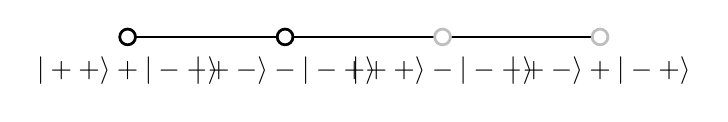
\begin{tikzpicture}  [scale=1]

\tikzstyle{every path}=[line width=1pt]

\newdimen\ms
\ms=0.1cm
\tikzstyle{s1}=[color=red,rectangle,inner sep=3.5]
\tikzstyle{c3}=[circle,inner sep={\ms/8},minimum size=4*\ms]
\tikzstyle{c2}=[circle,inner sep={\ms/8},minimum size=3*\ms]
\tikzstyle{c1}=[circle,inner sep={\ms/8},minimum size=2*\ms]
\tikzstyle{cs1}=[circle,inner sep={\ms/8},minimum size=1*\ms]

% Define positions of all observables

\coordinate (uu) at (0,0);
\coordinate (uv) at (2,0);
\coordinate (vu) at (4,0);
\coordinate (vv) at (6,0);

% draw contexts

\draw [color=black] (uu) -- (vv);

% draw atoms

\draw (uu) coordinate[c1,fill=white, draw=black,label=below:$\vert ++ \rangle + \vert -- \rangle$];
\draw (uv) coordinate[c1,fill=white, draw=black,label=below:$\vert +- \rangle - \vert -+ \rangle$];
\draw (vu) coordinate[c1,fill=white, draw=lightgray,label=below:$\vert ++ \rangle - \vert -- \rangle$];
\draw (vv) coordinate[c1,fill=white, draw=lightgray,label=below:$\vert +- \rangle + \vert -+ \rangle$];

\end{tikzpicture}
\end{center}
\caption{\label{2020-f-ghz-contextqmb}
Hypergraphs representing the single context associated with eigenstates of $\sigma_y \sigma_y$ (light gray indicates positive eigenvalues,
the respective states are fixed points).
}
\end{figure}


Nevertheless, I am quite certain that most experts would not agree with the conclusion that the GHZ argument is not different from stating that,
for pre-selected entangled particle pairs states the expectation of an observable ${{x}}^2$ can be negative,
although the single-particle expectation value of its constituents ${{x}}$ is a real number.
In this line of the query, the question remains: why should we not consider a quantum configuration involving such ``bare'' negative products of observables,
even without their ``dressing up'' with ``supporting'' co-observables and contexts
such as in~(\ref{2020-ghz-sigmas-contextop}), as substantial?




##########################################################################################


import cdd

mat = cdd.Matrix([
[-1 , -1, -1,  -1 ,  -1 ,  -1 ],
[-1 ,  1, -1,  -1 ,  -1 ,  -1 ]
[ 1 , -1,  1,   1 ,   1 ,   1 ],
[ 1 ,  1,  1,   1 ,   1 ,   1 ] ], number_type='fraction')

mat.rep_type = cdd.RepType.GENERATOR
poly = cdd.Polyhedron(mat)
print(poly)

ine = poly.get_inequalities()
print(ine)




###############################################################################################################################

u1 = (1/Sqrt[2]) Eigenvectors[PauliMatrix[1]][[1, 1]];
u2 = (1/Sqrt[2]) Eigenvectors[PauliMatrix[1]][[1, 2]];
v1 = (1/Sqrt[2]) Eigenvectors[PauliMatrix[1]][[2, 1]];
v2 = (1/Sqrt[2]) Eigenvectors[PauliMatrix[1]][[2, 2]];

c1 = (1/Sqrt[2]) Eigenvectors[PauliMatrix[2]][[1, 1]];
c2 = (1/Sqrt[2]) Eigenvectors[PauliMatrix[2]][[1, 2]];
d1 = (1/Sqrt[2]) Eigenvectors[PauliMatrix[2]][[2, 1]];
d2 = (1/Sqrt[2]) Eigenvectors[PauliMatrix[2]][[2, 2]];


u = {u1, u2}; v = {v1, v2}; UUp = {u, v};

c = {c1, c2}; d = {d1, d2}; CCp = {c, d};

C1p =  Flatten[
    Table[Flatten[
      KroneckerProduct[
       Flatten[KroneckerProduct[CCp[[i1]], CCp[[i2]]]],
       UUp[[i3]]]], {i3, 1, 2}, {i2, 1, 2}, {i1, 1, 2}], 2];

C2p =  Flatten[
    Table[Flatten[
      KroneckerProduct[
       Flatten[KroneckerProduct[CCp[[i1]], UUp[[i2]]]],
       CCp[[i3]]]], {i3, 1, 2}, {i2, 1, 2}, {i1, 1, 2}], 2];

C3p =  Flatten[
    Table[Flatten[
      KroneckerProduct[
       Flatten[KroneckerProduct[UUp[[i1]], CCp[[i2]]]],
       CCp[[i3]]]], {i3, 1, 2}, {i2, 1, 2}, {i1, 1, 2}], 2];

C4p =  Flatten[
    Table[Flatten[
      KroneckerProduct[
       Flatten[KroneckerProduct[UUp[[i1]], UUp[[i2]]]],
       UUp[[i3]]]], {i3, 1, 2}, {i2, 1, 2}, {i1, 1, 2}], 2];

TraditionalForm[C1p];

TraditionalForm[C2p];

TraditionalForm[C3p];

TraditionalForm[C4p];

###############################################################################################################################


psi=(1/Sqrt[2]){1,0,0,0,0,0,0,-1};



PMP122 = KroneckerProduct[ KroneckerProduct[ PauliMatrix[1] , PauliMatrix[2] ], PauliMatrix[2] ];
PMP212 = KroneckerProduct[ KroneckerProduct[ PauliMatrix[2] , PauliMatrix[1] ], PauliMatrix[2] ];
PMP221 = KroneckerProduct[ KroneckerProduct[ PauliMatrix[2] , PauliMatrix[2] ], PauliMatrix[1] ];
PMP111 = KroneckerProduct[ KroneckerProduct[ PauliMatrix[1] , PauliMatrix[1] ], PauliMatrix[1] ];


MatrixForm[PMP111]

antidiag111 = Table[ PMP111[[i,Length[PMP111]-i+1 ]],{i,Length[PMP111]}]

MatrixForm[PMP122]

antidiag122 = Table[ PMP122[[i,Length[PMP122]-i+1]],{i,Length[PMP122]} ]

MatrixForm[PMP212]

antidiag212 = Table[ PMP212[[i,Length[PMP212]-i+1]],{i,Length[PMP212]} ]

MatrixForm[PMP221]

antidiag221 = Table[ PMP221[[i,Length[PMP221]-i+1]],{i,Length[PMP221]} ]



PMP333 = KroneckerProduct[ KroneckerProduct[PauliMatrix[3], PauliMatrix[3]], PauliMatrix[3]];

MatrixForm[PMP333]

antidiag333 = Table[ PMP333[[i,i]],{i,Length[PMP333]} ]

PMP112 = KroneckerProduct[
   KroneckerProduct[PauliMatrix[1], PauliMatrix[1]], PauliMatrix[2]];
PMP121 = KroneckerProduct[
   KroneckerProduct[PauliMatrix[1], PauliMatrix[2]], PauliMatrix[1]];
PMP211 = KroneckerProduct[
   KroneckerProduct[PauliMatrix[2], PauliMatrix[1]], PauliMatrix[1]];
PMP222 = KroneckerProduct[
   KroneckerProduct[PauliMatrix[2], PauliMatrix[2]], PauliMatrix[2]];


MatrixForm[PMP222]

antidiag222 =
 Table[PMP222[[i, Length[PMP222] - i + 1]], {i, Length[PMP222]}]

MatrixForm[PMP112]

antidiag112 =
 Table[PMP112[[i, Length[PMP112] - i + 1]], {i, Length[PMP112]}]

MatrixForm[PMP121]

antidiag121 =
 Table[PMP121[[i, Length[PMP121] - i + 1]], {i, Length[PMP121]}]

MatrixForm[PMP211]

antidiag211 =
 Table[PMP211[[i, Length[PMP211] - i + 1]], {i, Length[PMP211]}]



antid={antidiag111,
       antidiag122,
       antidiag212,
       antidiag221,
       antidiag222,
       antidiag112,
       antidiag121,
       antidiag211};

MatrixForm[Table[antid[[i]].antid[[j]],{i,1,8},{j,1,8}]]


e={
{1, 0, 0, 0, 0, 0, 0, 1  } ,
{1, 0, 0, 0, 0, 0, 0, -1 } ,
{0, 1, 0, 0, 0, 0, 1, 0  } ,
{0, 1, 0, 0, 0, 0, -1, 0 } ,
{0, 0, 1, 0, 0, 1, 0, 0  } ,
{0, 0, 1, 0, 0, -1, 0, 0 } ,
{0, 0, 0, 1, 1, 0, 0, 0  } ,
{0, 0, 0, 1,- 1, 0, 0, 0 } };

MatrixForm[e]

PMP={PMP221,PMP212,PMP122,PMP111,PMP112,PMP121,PMP211,PMP222}

MatrixForm[
 Table[If[PMP[[i]].e[[j]] == e[[j]], 1, -1], {j, 1, 8}, {i, 1, 8}]]

MatrixForm[
 Table[If[PMP[[i]].e[[j]] == e[[j]], 1, -1], {j, 1, 8}, {i, 1, 4}]]


f={
{I, 0, 0, 0, 0, 0, 0, 1  } ,
{I, 0, 0, 0, 0, 0, 0, -1 } ,
{0, I, 0, 0, 0, 0, 1, 0  } ,
{0, I, 0, 0, 0, 0, -1, 0 } ,
{0, 0, I, 0, 0, 1, 0, 0  } ,
{0, 0, I, 0, 0, -1, 0, 0 } ,
{0, 0, 0, I, 1, 0, 0, 0  } ,
{0, 0, 0, I,- 1, 0, 0, 0 } };


MatrixForm[
 Table[If[PMP[[i]].f[[j]] == f[[j]], 1, -1], {j, 1, 8}, {i, 5, 8}]]





PMP122 . psi == psi

PMP212 . psi == psi

PMP221 . psi == psi

PMP111 . psi == -psi


es122 = Eigensystem[PMP122]

es212 = Eigensystem[PMP212]

es221 = Eigensystem[PMP221]

es111 = Eigensystem[PMP111]




MatrixForm[ev122]

TeXForm[MatrixForm[ev122]]

Print[TeXForm[MatrixForm[ev122]]];

ev212 = Eigenvectors[PMP212];

MatrixForm[ev212]

TeXForm[MatrixForm[ev212]]

Print[TeXForm[MatrixForm[ev212]]];

ev221 = Eigenvectors[PMP221];

MatrixForm[ev221]

Print[TeXForm[MatrixForm[ev221]]];

ev111 = Eigenvectors[PMP111];

MatrixForm[ev111]

Print[TeXForm[MatrixForm[ev111]]];


esall = Eigensystem[PMP122.PMP212.PMP221.PMP111.PMP122]


Table[ (psi. ev122[[i]])Conjugate[(psi. ev122[[i]])] ,{i,1,8}]


Table[ (psi. ev212[[i]])Conjugate[(psi. ev212[[i]])] ,{i,1,8}]


Table[ (psi. ev221[[i]])Conjugate[(psi. ev221[[i]])] ,{i,1,8}]


Table[ (psi. ev111[[i]])Conjugate[(psi. ev111[[i]])] ,{i,1,8}]






Adj122111 = Table[ ev111[[i]] . ev122[[j]] , {i,1,8},{j,1,8}];

TraditionalForm[ Adj122111 ]

Adj122122 = Table[ ev122[[i]] . ev122[[j]] , {i,1,8},{j,1,8}];

TraditionalForm[ Adj122122 ]

Adj122212 = Table[ ev122[[i]] . ev212[[j]] , {i,1,8},{j,1,8}];

TraditionalForm[ Adj122212 ]


##################################################################################################################


Eigenvectors[PauliMatrix[1]]
Eigenvectors[PauliMatrix[2]]
Eigenvectors[PauliMatrix[3]]



#################################################################################################################

https://pycddlib.readthedocs.io/en/latest/numbertype.html#cdd.NumberTypeable

import cdd;
mat = cdd.Matrix([
[1  ,  0  ,  0   ,      0  , 0 ,  0 ,  0 ] ,
[1  ,  1  ,  0   ,      0  , 0 ,  0 ,  0 ] ,
[1  ,  0  ,  1   ,      0  , 0 ,  0 ,  0 ] ,
[1  ,  1  ,  1   ,      0  , 0 ,  0 ,  0 ] ,
[1  ,  0  ,  0   ,      1  , 0 ,  0 ,  0 ] ,
[1  ,  1  ,  0   ,      1  , 0 ,  0 ,  0 ] ,
[1  ,  0  ,  1   ,      1  , 0 ,  0 ,  0 ] ,
[1  ,  1  ,  1   ,      1  , 0 ,  0 ,  0 ] ,
[1  ,  0  ,  0   ,      0  , 1 ,  0 ,  0 ] ,
[1  ,  1  ,  0   ,      0  , 1 ,  0 ,  0 ] ,
[1  ,  0  ,  1   ,      0  , 1 ,  0 ,  0 ] ,
[1  ,  1  ,  1   ,      0  , 1 ,  0 ,  0 ] ,
[1  ,  0  ,  0   ,      1  , 1 ,  0 ,  0 ] ,
[1  ,  1  ,  0   ,      1  , 1 ,  0 ,  0 ] ,
[1  ,  0  ,  1   ,      1  , 1 ,  0 ,  0 ] ,
[1  ,  1  ,  1   ,      1  , 1 ,  0 ,  0 ] ,
[1  ,  0  ,  0   ,      0  , 0 ,  1 ,  0 ] ,
[1  ,  1  ,  0   ,      0  , 0 ,  1 ,  0 ] ,
[1  ,  0  ,  1   ,      0  , 0 ,  1 ,  0 ] ,
[1  ,  1  ,  1   ,      0  , 0 ,  1 ,  0 ] ,
[1  ,  0  ,  0   ,      1  , 0 ,  1 ,  0 ] ,
[1  ,  1  ,  0   ,      1  , 0 ,  1 ,  0 ] ,
[1  ,  0  ,  1   ,      1  , 0 ,  1 ,  0 ] ,
[1  ,  1  ,  1   ,      1  , 0 ,  1 ,  0 ] ,
[1  ,  0  ,  0   ,      0  , 1 ,  1 ,  0 ] ,
[1  ,  1  ,  0   ,      0  , 1 ,  1 ,  0 ] ,
[1  ,  0  ,  1   ,      0  , 1 ,  1 ,  0 ] ,
[1  ,  1  ,  1   ,      0  , 1 ,  1 ,  0 ] ,
[1  ,  0  ,  0   ,      1  , 1 ,  1 ,  0 ] ,
[1  ,  1  ,  0   ,      1  , 1 ,  1 ,  0 ] ,
[1  ,  0  ,  1   ,      1  , 1 ,  1 ,  0 ] ,
[1  ,  1  ,  1   ,      1  , 1 ,  1 ,  0 ] ,
[1  ,  0  ,  0   ,      0  , 0 ,  0 ,  1 ] ,
[1  ,  1  ,  0   ,      0  , 0 ,  0 ,  1 ] ,
[1  ,  0  ,  1   ,      0  , 0 ,  0 ,  1 ] ,
[1  ,  1  ,  1   ,      0  , 0 ,  0 ,  1 ] ,
[1  ,  0  ,  0   ,      1  , 0 ,  0 ,  1 ] ,
[1  ,  1  ,  0   ,      1  , 0 ,  0 ,  1 ] ,
[1  ,  0  ,  1   ,      1  , 0 ,  0 ,  1 ] ,
[1  ,  1  ,  1   ,      1  , 0 ,  0 ,  1 ] ,
[1  ,  0  ,  0   ,      0  , 1 ,  0 ,  1 ] ,
[1  ,  1  ,  0   ,      0  , 1 ,  0 ,  1 ] ,
[1  ,  0  ,  1   ,      0  , 1 ,  0 ,  1 ] ,
[1  ,  1  ,  1   ,      0  , 1 ,  0 ,  1 ] ,
[1  ,  0  ,  0   ,      1  , 1 ,  0 ,  1 ] ,
[1  ,  1  ,  0   ,      1  , 1 ,  0 ,  1 ] ,
[1  ,  0  ,  1   ,      1  , 1 ,  0 ,  1 ] ,
[1  ,  1  ,  1   ,      1  , 1 ,  0 ,  1 ] ,
[1  ,  0  ,  0   ,      0  , 0 ,  1 ,  1 ] ,
[1  ,  1  ,  0   ,      0  , 0 ,  1 ,  1 ] ,
[1  ,  0  ,  1   ,      0  , 0 ,  1 ,  1 ] ,
[1  ,  1  ,  1   ,      0  , 0 ,  1 ,  1 ] ,
[1  ,  0  ,  0   ,      1  , 0 ,  1 ,  1 ] ,
[1  ,  1  ,  0   ,      1  , 0 ,  1 ,  1 ] ,
[1  ,  0  ,  1   ,      1  , 0 ,  1 ,  1 ] ,
[1  ,  1  ,  1   ,      1  , 0 ,  1 ,  1 ] ,
[1  ,  0  ,  0   ,      0  , 1 ,  1 ,  1 ] ,
[1  ,  1  ,  0   ,      0  , 1 ,  1 ,  1 ] ,
[1  ,  0  ,  1   ,      0  , 1 ,  1 ,  1 ] ,
[1  ,  1  ,  1   ,      0  , 1 ,  1 ,  1 ] ,
[1  ,  0  ,  0   ,      1  , 1 ,  1 ,  1 ] ,
[1  ,  1  ,  0   ,      1  , 1 ,  1 ,  1 ] ,
[1  ,  0  ,  1   ,      1  , 1 ,  1 ,  1 ] ,
[1  ,  1  ,  1   ,      1  , 1 ,  1 ,  1 ] ] ,
number_type='fraction');
mat.rep_type = cdd.RepType.GENERATOR;
poly = cdd.Polyhedron(mat);
ine= poly.get_inequalities();
print(ine);
f = open('C:/mytex/cdd/3-2-prob.ine', 'w');
s=str(ine);
f.write(s);
f.close();

H-representation
begin
 12 7 rational
 0 0 0 0 0 0 1
 0 1 0 0 0 0 0
 0 0 1 0 0 0 0
 0 0 0 1 0 0 0
 0 0 0 0 1 0 0
 0 0 0 0 0 1 0
 1 0 0 0 0 0 -1
 1 0 0 0 0 -1 0
 1 0 0 0 -1 0 0
 1 0 0 -1 0 0 0
 1 0 -1 0 0 0 0
 1 -1 0 0 0 0 0
end

######################################################################################


plus = {1, 0}; minus = {0, 1};
pm = {plus, minus};
Table[Flatten[
  KroneckerProduct[KroneckerProduct[pm[[i1]], pm[[i2]]], pm[[i3]]],
  2], {i1, 2}, {i2, 2}, {i3, 2}]

+ = {1,0}
- = {0,1}

+++ = {1, 0, 0, 0, 0, 0, 0, 0},
++- = {0, 1, 0, 0, 0, 0, 0, 0},
+-+ = {0, 0, 1, 0, 0, 0, 0, 0},
+-- = {0, 0, 0, 1, 0, 0, 0, 0},
-++ = {0, 0, 0, 0, 1, 0, 0, 0},
-+- = {0, 0, 0, 0, 0, 1, 0, 0},
--+ = {0, 0, 0, 0, 0, 0, 1, 0},
--- = {0, 0, 0, 0, 0, 0, 0, 1}


+++ + --- {1, 0, 0, 0, 0, 0, 0, 1},
+++ - --- {-1, 0, 0, 0, 0, 0, 0, 1},
++- + --+ {0, 1, 0, 0, 0, 0, 1, 0},
++- - --+ {0, -1, 0, 0, 0, 0, 1, 0},
+-+ + -+- {0, 0, 1, 0, 0, 1, 0, 0},
+-+ - -+- {0, 0, -1, 0, 0, 1, 0, 0},
+-- + -++ {0, 0, 0, 1, 1, 0, 0, 0},
+-- - -++ {0, 0, 0, -1, 1, 0, 0, 0}



xyy
+++ + --- {1, 0, 0, 0, 0, 0, 0, 1},
++- - --+ {0, -1, 0, 0, 0, 0, 1, 0},
+-+ - -+- {0, 0, -1, 0, 0, 1, 0, 0},
+-- + -++ {0, 0, 0, 1, 1, 0, 0, 0},

+++ - --- {-1, 0, 0, 0, 0, 0, 0, 1},
++- + --+ {0, 1, 0, 0, 0, 0, 1, 0},
+-+ + -+- {0, 0, 1, 0, 0, 1, 0, 0},
+-- - -++ {0, 0, 0, -1, 1, 0, 0, 0}

yxy
+++ + --- {1, 0, 0, 0, 0, 0, 0, 1},
++- - --+ {0, -1, 0, 0, 0, 0, 1, 0},
+-+ + -+- {0, 0, 1, 0, 0, 1, 0, 0},
+-- - -++ {0, 0, 0, -1, 1, 0, 0, 0},

+++ - --- {-1, 0, 0, 0, 0, 0, 0, 1},
++- + --+ {0, 1, 0, 0, 0, 0, 1, 0},
+-+ - -+- {0, 0, -1, 0, 0, 1, 0, 0},
+-- + -++ {0, 0, 0, 1, 1, 0, 0, 0}

yyx
+++ + --- {1, 0, 0, 0, 0, 0, 0, 1},
++- + --+ {0, 1, 0, 0, 0, 0, 1, 0},
+-+ - -+- {0, 0, -1, 0, 0, 1, 0, 0},
+-- - -++ {0, 0, 0, -1, 1, 0, 0, 0},

+++ - --- {-1, 0, 0, 0, 0, 0, 0, 1},
++- - --+ {0, -1, 0, 0, 0, 0, 1, 0},
+-+ + -+- {0, 0, 1, 0, 0, 1, 0, 0},
+-- + -++ {0, 0, 0, 1, 1, 0, 0, 0}

xxx
+++ - --- {-1, 0, 0, 0, 0, 0, 0, 1},
++- - --+ {0, -1, 0, 0, 0, 0, 1, 0},
+-+ - -+- {0, 0, -1, 0, 0, 1, 0, 0},
+-- - -++ {0, 0, 0, -1, 1, 0, 0, 0},

+++ + --- {1, 0, 0, 0, 0, 0, 0, 1},
++- + --+ {0, 1, 0, 0, 0, 0, 1, 0},
+-+ + -+- {0, 0, 1, 0, 0, 1, 0, 0},
+-- + -++ {0, 0, 0, 1, 1, 0, 0, 0}

check ###########################################################

(*
\vert +++ \rangle  + \vert --- \rangle &= \begin{pmatrix} 1, 0, 0, 0, 0, 0, 0, 1 \end{pmatrix}^\intercal ,  \\
\vert +++ \rangle  - \vert --- \rangle &= \begin{pmatrix} 1, 0, 0, 0, 0, 0, 0, -1 \end{pmatrix}^\intercal , \\
\vert ++- \rangle  + \vert --+ \rangle &= \begin{pmatrix} 0, 1, 0, 0, 0, 0, 1, 0 \end{pmatrix}^\intercal ,  \\
\vert ++- \rangle  - \vert --+ \rangle &= \begin{pmatrix} 0, 1, 0, 0, 0, 0, -1, 0 \end{pmatrix}^\intercal , \\
\vert +-+ \rangle  + \vert -+- \rangle &= \begin{pmatrix} 0, 0, 1, 0, 0, 1, 0, 0 \end{pmatrix}^\intercal ,  \\
\vert +-+ \rangle  - \vert -+- \rangle &= \begin{pmatrix} 0, 0, 1, 0, 0, -1, 0, 0 \end{pmatrix}^\intercal , \\
\vert +-- \rangle  + \vert -++ \rangle &= \begin{pmatrix} 0, 0, 0, 1, 1, 0, 0, 0 \end{pmatrix}^\intercal ,                   \\
\vert +-- \rangle  - \vert -++ \rangle &= \begin{pmatrix} 0, 0, 0, 1,- 1, 0, 0, 0 \end{pmatrix}^\intercal .

*)


PMP221 = KroneckerProduct[ KroneckerProduct[ PauliMatrix[2] , PauliMatrix[2] ], PauliMatrix[1] ];
PMP212 = KroneckerProduct[ KroneckerProduct[ PauliMatrix[2] , PauliMatrix[1] ], PauliMatrix[2] ];
PMP122 = KroneckerProduct[ KroneckerProduct[ PauliMatrix[1] , PauliMatrix[2] ], PauliMatrix[2] ];
PMP111 = KroneckerProduct[ KroneckerProduct[ PauliMatrix[1] , PauliMatrix[1] ], PauliMatrix[1] ];

e={
{1, 0, 0, 0, 0, 0, 0, 1  } ,
{1, 0, 0, 0, 0, 0, 0, -1 } ,
{0, 1, 0, 0, 0, 0, 1, 0  } ,
{0, 1, 0, 0, 0, 0, -1, 0 } ,
{0, 0, 1, 0, 0, 1, 0, 0  } ,
{0, 0, 1, 0, 0, -1, 0, 0 } ,
{0, 0, 0, 1, 1, 0, 0, 0  } ,
{0, 0, 0, 1,- 1, 0, 0, 0 } };



Table[{
If[PMP221.e[[i]] == e[[i]],+1,-1],
If[PMP212.e[[i]] == e[[i]],+1,-1],
If[PMP122.e[[i]] == e[[i]],+1,-1],
If[PMP111.e[[i]] == e[[i]],+1,-1]},
{i,1,8}]    //MatrixForm

Table[{
If[PMP221.e[[i]] == -e[[i]],+1,-1],
If[PMP212.e[[i]] == -e[[i]],+1,-1],
If[PMP122.e[[i]] == -e[[i]],+1,-1],
If[PMP111.e[[i]] == -e[[i]],+1,-1]},
{i,1,8}]   //MatrixForm


#######################################################################
2 factor attempts
#######################################################################

PMP21 =  KroneckerProduct[ PauliMatrix[2] , PauliMatrix[1] ];
PMP12 =  KroneckerProduct[ PauliMatrix[1] , PauliMatrix[2] ];
PMP11 =  KroneckerProduct[ PauliMatrix[1] , PauliMatrix[1] ];

Eigensystem[PMP21]

Eigensystem[PMP12]

Eigensystem[PMP11]

PMP22 =  KroneckerProduct[ PauliMatrix[2] , PauliMatrix[2] ];
Eigensystem[PMP22]


#################################################################################



(* GHZ game *)

z1p = (x1p + x1m); z1m = (x1p - x1m);
z2p = (x2p + x2m); z2m = (x2p - x2m);
z3p = (x3p + x3m); z3m = (x3p - x3m);
FullSimplify[z1p*z2p*z3p + z1m*z2m*z3m]


z1p = (x1p + x1m); z1m = (x1p - x1m);
z2p = (y2p + y2m); z2m = (-I)(y2p - y2m);
z3p = (y3p + y3m); z3m = (-I)(y3p - y3m);
FullSimplify[z1p*z2p*z3p + z1m*z2m*z3m]


z1p = (y1p + y1m); z1m = (-I)(y1p - y1m);
z2p = (x2p + x2m); z2m = (x2p - x2m);
z3p = (y3p + y3m); z3m = (-I)(y3p - y3m);
FullSimplify[z1p*z2p*z3p + z1m*z2m*z3m]

z1p = (y1p + y1m); z1m = (-I)(y1p - y1m);
z2p = (y2p + y2m); z2m = (-I)(y2p - y2m);
z3p = (x3p + x3m); z3m = (x3p - x3m);
FullSimplify[z1p*z2p*z3p + z1m*z2m*z3m]

(* variant  e8 *)

z1p = (x1p + x1m); z1m = (x1p - x1m);
z2p = (x2p + x2m); z2m = (x2p - x2m);
z3p = (x3p + x3m); z3m = (x3p - x3m);
FullSimplify[z1p*z2m*z3m - z1m*z2p*z3p]


z1p = (x1p + x1m); z1m = (x1p - x1m);
z2p = (y2p + y2m); z2m = (-I)(y2p - y2m);
z3p = (y3p + y3m); z3m = (-I)(y3p - y3m);
FullSimplify[z1p*z2m*z3m - z1m*z2p*z3p]

z1p = (y1p + y1m); z1m = (-I)(y1p - y1m);
z2p = (x2p + x2m); z2m = (x2p - x2m);
z3p = (y3p + y3m); z3m = (-I)(y3p - y3m);
FullSimplify[z1p*z2m*z3m - z1m*z2p*z3p]

z1p = (y1p + y1m); z1m = (-I)(y1p - y1m);
z2p = (y2p + y2m); z2m = (-I)(y2p - y2m);
z3p = (x3p + x3m); z3m = (x3p - x3m);
FullSimplify[z1p*z2m*z3m - z1m*z2p*z3p]





#######################################################################

Reduce[
y1 y2 x3 == -1 &&
y1 x2 y3 == -1 &&
x1 y2 y3 == -1 &&
x1 x2 x3 == -1 ,
{x1,x2,x3,y1,y2,y3}, Integers]

Reduce[
y1 y2 x3 == -1 &&
y1 x2 y3 == -1 &&
x1 y2 y3 == 1 &&
x1 x2 x3 == 1 ,
{x1,x2,x3,y1,y2,y3}, Integers]

Reduce[
y1 y2 x3 == -1 &&
y1 x2 y3 == 1 &&
x1 y2 y3 == 1 &&
x1 x2 x3 == -1 ,
{x1,x2,x3,y1,y2,y3}, Integers]

Reduce[
y1 y2 x3 == -1 &&
y1 x2 y3 == 1 &&
x1 y2 y3 == -1 &&
x1 x2 x3 == 1 ,
{x1,x2,x3,y1,y2,y3}, Integers]

Reduce[
y1 y2 x3 == 1 &&
y1 x2 y3 == -1 &&
x1 y2 y3 == 1 &&
x1 x2 x3 == -1 ,
{x1,x2,x3,y1,y2,y3}, Integers]

Reduce[
y1 y2 x3 == 1 &&
y1 x2 y3 == -1 &&
x1 y2 y3 == -1 &&
x1 x2 x3 == 1 ,
{x1,x2,x3,y1,y2,y3}, Integers]

Reduce[
y1 y2 x3 == 1 &&
y1 x2 y3 == 1 &&
x1 y2 y3 == -1 &&
x1 x2 x3 == -1 ,
{x1,x2,x3,y1,y2,y3}, Integers]


Reduce[
y1 y2 x3 == 1 &&
y1 x2 y3 == 1 &&
x1 y2 y3 == 1 &&
x1 x2 x3 == 1 ,
{x1,x2,x3,y1,y2,y3}, Integers]


################################################

ClearAll[AntidiagonalMatrix]
AntidiagonalMatrix[list : (_List | _SparseArray)] :=
 AntidiagonalMatrix[list, 0]
AntidiagonalMatrix[list : (_List | _SparseArray), k_Integer] :=
 Reverse[DiagonalMatrix[list, k], 2]
AntidiagonalMatrix[list : (_List | _SparseArray), k_Integer,
  n_Integer] := AntidiagonalMatrix[list, k, {n, n}]
AntidiagonalMatrix[list : (_List | _SparseArray), k_Integer,
  mn : {m_Integer, n_Integer}] :=
 Reverse[DiagonalMatrix[list, k, mn], 2]

aa = AntidiagonalMatrix[{-1, -1, 1, 1, 1, 1, -1, -1}];
bb = AntidiagonalMatrix[{-1, 1, -1, 1, 1, -1, 1, -1}];
cc = AntidiagonalMatrix[{-1, 1, 1, -1, -1, 1, 1, -1}];
dd = AntidiagonalMatrix[{1, 1, 1, 1, 1, 1, 1, 1}];

Commutator[a_, b_] := a.b - b.a;

Commutator[aa, bb]
Commutator[aa, cc]
Commutator[aa, dd]
Commutator[bb, cc]
Commutator[bb, dd]
Commutator[cc, dd]




############################################################

xp = {1,1}; xm = {1,-1}; yp = {1,I}; ym = {1,-I};

contexts = {};

con1 = {
{
Flatten[ KroneckerProduct[ xp , Flatten[ KroneckerProduct[ xp , xp ]]]],
Flatten[ KroneckerProduct[ xp , Flatten[ KroneckerProduct[ xm , xm ]]]],
Flatten[ KroneckerProduct[ xm , Flatten[ KroneckerProduct[ xp , xm ]]]],
Flatten[ KroneckerProduct[ xm , Flatten[ KroneckerProduct[ xm , xp ]]]]},
{
Flatten[ KroneckerProduct[ xm , Flatten[ KroneckerProduct[ ym , ym ]]]],
Flatten[ KroneckerProduct[ xm , Flatten[ KroneckerProduct[ yp , yp ]]]],
Flatten[ KroneckerProduct[ xp , Flatten[ KroneckerProduct[ ym , yp ]]]],
Flatten[ KroneckerProduct[ xp , Flatten[ KroneckerProduct[ yp , ym ]]]]},
{
Flatten[ KroneckerProduct[ ym , Flatten[ KroneckerProduct[ xm , ym ]]]],
Flatten[ KroneckerProduct[ ym , Flatten[ KroneckerProduct[ xp , yp ]]]],
Flatten[ KroneckerProduct[ yp , Flatten[ KroneckerProduct[ xm , yp ]]]],
Flatten[ KroneckerProduct[ yp , Flatten[ KroneckerProduct[ xp , ym ]]]]},
{
Flatten[ KroneckerProduct[ ym , Flatten[ KroneckerProduct[ ym , xm ]]]],
Flatten[ KroneckerProduct[ ym , Flatten[ KroneckerProduct[ yp , xp ]]]],
Flatten[ KroneckerProduct[ yp , Flatten[ KroneckerProduct[ ym , xp ]]]],
Flatten[ KroneckerProduct[ yp , Flatten[ KroneckerProduct[ yp , xm ]]]]
}} ;


TensorProductVec[x_, y_] :=
  Flatten[Table[
    x[[i]] y[[j]], {i, 1, Length[x]}, {j, 1, Length[y]}]];

con2 = {
{
TensorProductVec[ xp , TensorProductVec[ xp , xp ]],
TensorProductVec[ xp , TensorProductVec[ xm , xm ]],
TensorProductVec[ xm , TensorProductVec[ xp , xm ]],
TensorProductVec[ xm , TensorProductVec[ xm , xp ]]},
{
TensorProductVec[ xm , TensorProductVec[ ym , ym ]],
TensorProductVec[ xm , TensorProductVec[ yp , yp ]],
TensorProductVec[ xp , TensorProductVec[ ym , yp ]],
TensorProductVec[ xp , TensorProductVec[ yp , ym ]]},
{
TensorProductVec[ ym , TensorProductVec[ xm , ym ]],
TensorProductVec[ ym , TensorProductVec[ xp , yp ]],
TensorProductVec[ yp , TensorProductVec[ xm , yp ]],
TensorProductVec[ yp , TensorProductVec[ xp , ym ]]},
{
TensorProductVec[ ym , TensorProductVec[ ym , xm ]],
TensorProductVec[ ym , TensorProductVec[ yp , xp ]],
TensorProductVec[ yp , TensorProductVec[ ym , xp ]],
TensorProductVec[ yp , TensorProductVec[ yp , xm ]]
}} ;

con1 == con2

MatrixForm[Table[ con1[[1,i]] . Conjugate[ con1[[1,j]] ], {i,4},{j,4}]]

MatrixForm[Table[ con1[[2,i]] . Conjugate[ con1[[2,j]] ], {i,4},{j,4}]]

MatrixForm[Table[ con1[[3,i]] . Conjugate[ con1[[3,j]] ], {i,4},{j,4}]]

MatrixForm[Table[ con1[[4,i]] . Conjugate[ con1[[4,j]] ], {i,4},{j,4}]]

contexts = {};

Do[
Do[
Do[
Do[

If[ con1[[1,i1]] . Conjugate[ con1[[2,i2]] ] == 0,
If[ con1[[1,i1]] . Conjugate[ con1[[3,i3]] ] == 0,
If[ con1[[1,i1]] . Conjugate[ con1[[4,i4]] ] == 0,

If[ con1[[2,i2]] . Conjugate[ con1[[3,i3]] ] == 0,
If[ con1[[2,i2]] . Conjugate[ con1[[4,i4]] ] == 0,

If[ con1[[3,i3]] . Conjugate[ con1[[4,i4]] ] == 0,  AppendTo[contexts, {i1, i2, i3, i4}]
]]]]]]

,{i4,4}]
,{i3,4}]
,{i2,4}]
,{i1,4}]

contexts

{{1, 1, 1, 1}, {1, 2, 3, 4}, {2, 1, 4, 3}, {2, 2, 2, 2}, {3, 3, 3, 3}, {3, 4, 1, 2}, {4, 3, 2, 1}, {4, 4, 4, 4}}


#################################

Pasting of 7 blocks
16 atoms
10 blocks
 0 proper subsets of blocks
 4   1  2  3  4
 4   5  6  7  8
 4   9 10 11 12
 4  13 14 15 16
 4   1  5  9 13
 4   2  6 10 14
 4   3  7 11 15
 4   4  8 12 16
 4   3  8  9 14
 4   2  5 12 15
8 2-valued evaluations of atoms:
1 0 0 0 0 0 1 0 0 0 0 1 0 1 0 0
1 0 0 0 0 0 0 1 0 1 0 0 0 0 1 0
0 1 0 0 0 0 1 0 1 0 0 0 0 0 0 1
0 1 0 0 0 0 0 1 0 0 1 0 1 0 0 0
0 0 1 0 1 0 0 0 0 1 0 0 0 0 0 1
0 0 1 0 0 1 0 0 0 0 0 1 1 0 0 0
0 0 0 1 1 0 0 0 0 0 1 0 0 1 0 0
0 0 0 1 0 1 0 0 1 0 0 0 0 0 1 0

set of 2-valued evaluations of atoms:
nonempty: yes
unital: yes
separating atoms: yes
separating: no for sets of atoms (different elements?)
 3+4/5+6
 2+4/9+11
 2+3/13+16
 1+4/14+15
 1+3/10+12
 1+2/7+8
 6+8/13+15
 6+7/9+12
 5+8/10+11
 5+7/14+16
 11+12/13+14
 9+10/15+16
 9+13/2+6
 5+13/3+11
 5+9/4+16
 1+13/8+12
 1+9/7+15
 1+5/10+14
 6+14/4+12
 6+10/3+15
 2+14/7+11
 2+10/8+16
 11+15/4+8
 3+7/12+16
 8+9/2+15
 3+14/5+12


vecfind -4d -vgen=1,-1,0,2,-2,3,-3,4,-4 < ghz.in

1234,5678,9ABC,DEFG,159D,26AE,37BF,48CG,389E,25CF.

c:\mytex\mmp>vecfind -4d -vgen=0,1,-1 < 18-9.mmp
#1 pass:: 1234,4567,789A,ABCD,DEFG,GHI1,35CE,29BI,68FH.{
1={0,0,0,1},2={0,0,1,0},3={1,1,0,0},4={1,-1,0,0},5={0,0,1,1},
6={1,1,1,-1},7={1,1,-1,1},8={1,-1,1,1},9={1,0,0,-1},
A={0,1,1,0},B={1,0,0,1},C={1,-1,1,-1},D={1,1,-1,-1},
E={1,-1,-1,1},F={0,1,0,1},G={1,0,1,0},H={1,0,-1,0},I={0,1,0,0}}

%%%%%%%%%%%%%%%%%%%%%%%%%%%%%%%%%%%%%%%%%%%%%%%%%%%%%%%%%%%%%%%%%%%%%%%

xp = {1,1}; xm = {1,-1}; yp = {1,I}; ym = {1,-I};

Flatten[ KroneckerProduct[ xp , xp ]]

Flatten[ KroneckerProduct[ xm , xm ]]

Flatten[ KroneckerProduct[ xp , xm ]]

Flatten[ KroneckerProduct[ xm , xp ]]


Flatten[ KroneckerProduct[ yp , yp ]]

Flatten[ KroneckerProduct[ ym , ym ]]

Flatten[ KroneckerProduct[ yp , ym ]]

Flatten[ KroneckerProduct[ ym , yp ]]


Flatten[ KroneckerProduct[ yp , xp ]]

Flatten[ KroneckerProduct[ ym , xm ]]

Flatten[ KroneckerProduct[ yp , xm ]]

Flatten[ KroneckerProduct[ ym , xp ]]


Flatten[ KroneckerProduct[ xp , yp ]]

Flatten[ KroneckerProduct[ xm , ym ]]

Flatten[ KroneckerProduct[ xp , ym ]]

Flatten[ KroneckerProduct[ xm , yp ]]


#################################################################

(* reduced  GHZ game *)

z1p = (x1p + x1m); z1m = (x1p - x1m);
z2p = (x2p + x2m); z2m = (x2p - x2m);
FullSimplify[z1p*z2p + z1m*z2m + z1p*z2m + z1m*z2p]


z1p = (x1p + x1m); z1m = (x1p - x1m);
z2p = (y2p + y2m); z2m = (-I)(y2p - y2m);
FullSimplify[z1p*z2p + z1m*z2m + z1p*z2m + z1m*z2p]


z1p = (y1p + y1m); z1m = (-I)(y1p - y1m);
z2p = (x2p + x2m); z2m = (x2p - x2m);
FullSimplify[z1p*z2p + z1m*z2m + z1p*z2m + z1m*z2p]

z1p = (y1p + y1m); z1m = (-I)(y1p - y1m);
z2p = (y2p + y2m); z2m = (-I)(y2p - y2m);
FullSimplify[z1p*z2p + z1m*z2m + z1p*z2m + z1m*z2p]

%%%%%%%%%%%%%%%%%%%%%%%%%%%%%%%%%%%%%%%%%%%%%%%%%%%%%%%%%%%%%%%%%%%%%%%%%%%%

Dear Dr. M�ller,

I have revised the manuscript according to the critical reviews and suggestions of the two Referees and the input of other colleagues.
In particular, I have tried to emphasize the semantic content, the "take-home" message, for the reader.

The paper has been restructured at the beginning, first expressing what I had in mind and a motivation for why one might consider this.

Then, I have recast arguments and Figure 2 to improve comprehensibility and clarity.

I have also added a passage at the end, thereby using explicitly the terms suggested by the Second Referee because I believe that this is very helpful in understanding the intent of the investigation:

"This review is the continuation of an ongoing effort...

Following the aforementioned effort, the conceptual take-home message of the paper is this: the GHZ argument can be readily ``embedded'' into,
or translated and presented, in terms of the quantum logical framework of Birkhoff and von Neumann~\cite{birkhoff-36}
as well as partial algebras~\cite{kochen2,kochen3} and orthomodular structures~\cite{kalmbach-83,pulmannova-91}.
From a formal point of view, this allows its uniform presentation and comparison to ``competing'' and related arguments,
such as Hardy-type or KS arguments.
From an empirical point of view, the operator-based approach facilitates operational extensions and generalizations of the original argument."

I very much hope that, with these revisions, the paper can be accepted in its present form.

Please do not hesitate to contact me again should further revisions be necessary.

I kindly thank you and the Referees for their kind, valuable input, and the attention dedicated to this manuscript.

Yours Sincerely,

Karl Svozil

